\documentclass{report}
\usepackage{suthesis}
\usepackage{amsmath}
\usepackage{graphicx}

\dept{Music}

\begin{document}
\title{Mathematical models of rhythm synchronization and anticipation}
\author{Iran R. Roman}
\principaladviser{Chris Chafe}
\firstreader{Edward W. Large}
\secondreader{Julius O. Smith}

\beforepreface

\prefacesection{Abstract}
When humans synchronize with a periodic stimulus, endogenous processes like neural delays and spontaneous rates are related to the systematic asynchronies observed between human movements and stimulus onsets. This dissertation presents two different models that capture how neural delays and spontaneous rates of movement affect human synchronization. Additionally, these models have been implemented with tensorflow 2, allowing for parameter optimization and general applications in signal processing algorithms.

The first model captures how, in metronome synchronization tasks, people tend to tap slightly before the metronome clicks. This anticipation tendency increases with longer stimulus periods of up to 3500ms, but is less pronounced in trained individuals like musicians compared to non-musicians. In non-biological systems, anticipation is observed between delayed-coupled systems. Therefore, the human anticipation tendency could be explained with such a system because delayed communication is inherent to the sensorimotor system during perception-action coordination. This dissertation tests this hypothesis with a dynamical systems model consisting of an oscillator receiving its own delayed activity as input. Simulation experiments were conducted using previously published behavioral data from human studies with either synchronization to a metronome or interpersonal synchronization. Our new model is validated by its ability to simulate real human synchronization and anticipation data. As a result, our model informs theories of adaptive human synchronization.

The second model captures how interpersonal synchronization is affected by an individual's spontaneous rates of movement. Specifically, the greater discrepancy between two synchronizing musicians' spontaneous rates, the greater asynchronies observed during joint duet performance. Interestingly, a musician's spontaneous rate remains stable after experiencing a joint performance, suggesting short-term tempo adaptation during joint performance and spontaneous rate restoration afterwards. This dissertation tests whether an oscillatory dynamical system with frequency elasticity and hebbian learning could explain how spontaneous rates affect interpersonal synchronization. The model consists of an oscillator with a natural frequency that emulates the human spontaneous rate. The oscillator's frequency term is elastic to allow for short-term frequency changes during synchronization with a periodic stimulus of an arbitrary frequency. However, elasticity makes the oscillator return to its original natural frequency when it is no longer stimulated. Our model is validated by its ability to simulate human synchronization data using its adaptive and elastic frequency learning mechanism. This model can simulate duet musical performance and capture how asynchronies between performers are systematically influenced by the difference between two performers' spontaneous rates.

Finally, this dissertation presents a novel implementation of these oscillatory models in tensorflow 2. This toolbox is written with a broad user-base in mind, and it includes general numerical methods for integration of ordinary differential equations. Besides allowing users to simulate different types of neural oscillators in multi-scale networks, the toolbox also allows oscillatory models to be combined with deep learning networks for the first time. Oscillatory networks are a new alternative for time-frequency analysis in deep learning algorithms, and can improve performance in common signal processing tasks.

\prefacesection{Acknowledgments}
I would like to thank my colleagues, family, and friends. Thank you to my CCRMA cohort of Ph.D. candidates: Kitty Shi and Tim O'Brien. Similarly, I want to thank all my CCRMA friends: Auriel Washburn, Orchi Das, Madeline Huberth, Alex Chechile, Wisam Reid, Cynthia Moncada, Shu Yu Lin, Nick Gang, Ethan Geller, Rahul Agnihotri, Emily Graber, John Granzow, Woody Herman, Kai-Chieh Huang, Jay Kadis, Sasha Leitman, Sara Mart\'{i}n, Romain Michon, Dave Kerr, Fernando Lopez-Lezcano, Carr Wilkerson, Elliot Kermit-Canfield, Eoin Callery, Jorge Herrera, Rob Hamilton, Chryssie Nanou, Christopher Jette, Matt Wright, Nette Worthey, Mario Champagne, Velda Williams, and Debbie Barney. 

Outside of CCRMA, I want to thank members of the Bioscience community: Samar Fahmy, Terrance Mayes, Dr. Tim Stearns, Dr. Ayodele Thomas, and Dr. Tony Ricci. I also want to say thank you to Dr. Jay McClelland for letting me participate and learn in this lab meetings.

A big thank you to the Stanford Human-Centered Artificial Intelligence initiative for funding the last year of my Ph.D. studies, the Howard Hughes Medical Institute for funding my first academic quarter at Stanford, and the Center for Mind, Brain, Computation and Technology for financial support to travel to conferences and access computational tools. 

I also want to thank CCRMA faculty. Thank you Malcolm Slaney and Takako Fujioka for providing critical feedback and advice to my modeling work presented in this dissertation. Thanks for Jonathan Abel and David Berners for letting me serve as their teaching assistant of signal processing. Thank you Jonathan Berger and Jaroslaw Kapuscinski for always being supportive and providing me with general academic advice. Thank you Ge Wang for your courses where I learned the fundamentals of algorithms applied to digital sound. 

My dissertation committee deserves a big thank you for all their work guiding my Ph.D. research. Thank you Julius Smith for inspiring me to always extend my horizons and for being an excellent role model of scholarship and creative thinking. Thank you Edward W. Large for always being supportive of my research efforts and guiding me whenever I felt lost. And thank you to Chris Chafe for trusting in my ideas and letting me shape my research agenda. 

My journey at Stanford was possible thanks to the support that my family gave me. Thank you Alejandra Torres for being the most caring and sincere individual I have ever met, and thank you for always being there to support me and guide me. Thank you Iran A. Roman for bringing joy to all my days and for teaching me so much about everything. I also want to thank my supportive and loving parents: Adriana Guzman Guzman and Iran Manuel Roman Jaimes. Finally, thank you to my brothers Rodolfo, Rodrigo, and Adrian.

\afterpreface

\chapter{Introduction}
\chaptermark{Introduction}

Humans carry out periodic actions everyday. Some of these actions are spontaneously paced, like walking, blinking, or swimming. Others are paced by external factors, like music when we dance, or other individuals when we perform crew rowing or play in a musical ensemble. Periodic actions are ubiquitous in human behavior, and they are an integral part of the most basic human functions (i.e., breathing, chewing, running) and the most complex social interactions (i.e., music making, military marching, or turn-taking conversing).

Every person has a different walking or blinking speed. This suggests that spontaneous periodic actions are influenced by personal factors, like anatomy and function of the body \cite{goodman2000advantages} and the brain \cite{latash1992virtual}, which in turn are influenced by one's genetics and the environment. These internal factors seem to be flexible though, allowing a person to carry out periodic actions at different rates when synchronizing movements with another person or with an external stimulus like music or a metronome. 

Previous research of human periodic actions has identified behavioral patterns. For example, while synchronizing with a simple periodic stimulus, like a metronome, humans show a tendency to anticipate the stimulus with their actions \cite{repp2007tapping}. Additionally, the difference between a person's spontaneous motor tempo (SMT) and the stimulus tempo determines whether a person will anticipate or lag such a stimulus when synchronizing with it \cite{scheurich2018tapping}. Finally, when spontaneously performing a periodic action at a tempo different than the SMT, humans tend to drift back to the SMT \cite{zamm2018musicians}. 

These patterns and phenomena observed across different behavioral experiments suggest that there are  mechanisms at play when humans carry out periodic actions. However, currently there are conflicting views between models trying to explain the computational and dynamical origins of periodic action, synchronization, and anticipation. This dissertation presents dynamical equations to shed light on possible biophysical mechanisms that explain how internal and external factors affect human periodic action. 

\section{Summary of chapters}

This dissertation presents simple mathematical models, consisting of oscillatory equations with dynamic mechanisms, that capture human periodic synchronization and anticipation. One chapter of this dissertation also describes how these models can be combined to build a more general and robust model of human periodic action. Additionally, the tools developed to simulate these mathematical models serve as the foundation for future research using these oscillatory models to simulate human behavior and other dynamic phenomena. Finally, we also describe how these oscillatory equations can be used for signal processing, and as building blocks in artificial intelligence algorithms like deep neural networks.

\subsection{Chapter 1}
Here, in this introduction, we discuss the scope and structure of this dissertation, as well as previous modeling work trying to explain human periodic synchronization and anticipation.

\subsection{Chapter 2}
The first model presented in this dissertation captures the humans tendency to anticipate periodic events. When an individual synchronizes a body movement (i.e., finger taps) with a metronome, the individual's actions tend to precede the metronome clicks. This anticipation tendency is observed for metronome inter-onset-intervals lengths ranging from 500ms to 3500ms \cite{repp2005sensorimotor}, and tends to be smaller among musicians than among non-musicians \cite{repp2007tapping}. Interestingly, similar anticipation tendencies have been observed in the field of physics when a system with delayed feedback synchronizes with a periodic signal (i.e., two coupled lasers where one of the lasers receives its own delayed output as input) \cite{stepp2010strong}. Considering this, we hypothesized that the human anticipation tendency is the result of delayed neural signals traveling back and forth between an individual's motor effectors (i.e., finger tips) and the motor cortex. To test this hypothesis, we designed a mathematical model consisting of an oscillator with delayed feedback. The oscillator emulates periodic motor activity, and the delayed feedback simulates the axonal communication in the brain's motor system. When stimulating this model with the same metronome rates that humans synchronize with, the model showed the same anticipatory tendencies observed in musicians. Additionally, by increasing the delayed feedback amplitude we observed the anticipatory tendency shown by non-musicians. To validate the model, we simulated multiple musical performance tasks where the anticipatory tendency has been observed in humans. Finally, the model can also make predictions, including interpersonal synchronization settings that have not been studied in humans.

\subsection{Chapter 3}
The second model captures how an individual's spontaneous motor tempo (SMT) affects synchronization. Humans can spontaneously perform a simple melody showing an SMT. The origins of the SMT are still under investigation, with much debate sorrounding them \cite{scheurich2018tapping}. Possible mechanisms of the SMT include body anatomy and the brain's central pattern generators \cite{scheurich2018tapping}. Interestingly, the SMT is consistent throughout adulthood \cite{scheurich2018tapping}. Musicians can spontaneously perform a simple melody that reflects their SMT \cite{scheurich2018tapping}. While humans can synchronize their movements with stimuli at different frequencies, behavioral research shows that the SMT systematically affects how an individual synchronizes. For example, individuals have a tendency to anticipate a stimulus frequency slower than the SMT, and lag a stimulus frequency faster than the SMT \cite{scheurich2018tapping}. This behavioral data suggests that humans can adaptively synchronize with an arbitrary stimulus tempo, but that the SMT acts as a constant pulling force. Considering this, we hypothesized that this phenomena can be explained with two dynamical mechanisms: Hebbian learning for tempo adaptation and elasticity. To test this hypothesis, we designed a mathematical model consisting of an oscillator with Hebbian learning and elasticity that control the oscillator's frequency. This model simulates the brain's ability to synchronize neural activity with the period of an external stimulus while maintaining the SMT in the absence of a stimulus. We used this model to simulate music performance tasks originally designed to study how the SMT affects human synchronization with a metronome or between musicians. The model was able to simulate the patterns observed in human data across different music performance tasks and was also able to make predictions that can be tested by collecting new human data.

\subsection{Chapter 4}
This chapter describes how the models described in chapters 2 and 3 can be combined to create a single, parsimonious, and dynamical model of human synchronization. Because the models are built with simple dynamic principles and validated with real human data, combining them will result in a model that will generalize across periodic action and/or synchronization tasks that humans can conceivably carry out. This model should be able to make predictions of human behavior that could be validated with new human data.

\subsection{Chapter 5}
The last chapter of this dissertation describes a new software toolbox that was written to build oscillatory models and optimize them using automatic differentiation. This toolbox was implemented in tensorflow 2, which was originally written to develop artificial intelligence algorithms and is the most advanced tool to build large network models. This toolbox allows the user, for the first time, to optimize oscillator models using human data targets. It also allows for future research using dynamic models as building blocks in artificial intelligence algorithms. This last chapter also presents an experiment where a dynamic model of neural oscillators is used to clean noisy speech. This proof of concept expands the possible ways to optimize oscillatory models beyond modeling of human behavior. 

\subsection{Chapter 6}
This chapter is the concluson of this dissertation. It summarizes the main findings of each chapter and the contributions of this dissertation.

\section{Literature review}

Every chapter in this document reviews the relevant literature. In this introductory chapter we give a broad overview of previous models of human anticipation and synchronization.

\subsection{Models of anticipation}
Humans have a natural tendency to anticipate events. A general definition of anticipation is ``the forecast of a future event". From a statistical perspective, anticipation involves previous knowledge about the likelihood of an event. Hence, anticipation in the statistical sense is inference from previous knowledge or evidence \cite{cox2006principles}. Karl Friston and colleagues have suggested that the brain carries out a complex and explicit mechanism of anticipation based on statistical inference \cite{maffei2017perceptual}. In their view, anticipation is a human cognitive process that involves statistical analysis of multisensory cues with the explicit goal of anticipating an event. Consistent with this perspective, multiple models of human anticipation carry out probabilistic computations on inputs. Examples include a Bayesian model of sensorimotor integration during movement learning \cite{kording2004bayesian}, and a recurrent neural network model of human anticipation and synchronization with a robot \cite{schydlo2018anticipation}. 

However, anticipation may be the result of simpler biomechanical properties. In the specific case of the anticipatory tendency observed when humans synchronize finger taps with a metronome, anticipation could be explained by the time difference in communication between the auditory and peripheral motor systems \cite{aschersleben2002temporal}. It takes less time for the metronome sounds to reach the auditory cortex than the fingertip feedback to reach the motor cortex. As a result, taps must anticipate metronome clicks so that the fingertip feedback and the metronome clicks reach the brain's multisensory association areas at the same time \cite{aschersleben2002temporal}. This simple model could explain anticipation by considering the nervous system anatomy without the need for complicated and explicit statistical computations. However, research has shown that this is not the mechanism because this model predicts that signal loudness has an effect on anticipation, and this prediction was not observed in empirical data \cite{bialunska2011increasing}. The model presented in chapter 2 of this dissertation incorporates delays in a dynamical system constrained by the simple mechanism of `strong anticipation'. 

\subsection{Strong anticipation}
The kind of anticipation that emerges in a system as a result of its structure and function is known as `strong anticipation' \cite{dubois2001incursive}. If anticipation emerges in a system as a result of statistical inference, then the system is carrying out `weak anticipation' \cite{dubois2001incursive}. Stepp and Turvey \cite{stepp2010strong} emphasized that in neuroscience, anticipation is assumed to be `weak anticipation' and most models ignore the structure and function of anticipatory systems. Because anticipation is observed even in non-living systems (i.e., systems unable to carry out statistical inference), assuming that human anticipation is the result of `weak anticipation' is a limited perspective. Stepp and Turvey \cite{stepp2010strong} have demonstrated that anticipation, in general, can be observed in delayed coupled systems (i.e., a system receiving both a stimulus and its own delayed activity as input). When humans synchronize with a metronome, neural signals must travel back and forth across myelinated axons as long as 1 meter in length, with speeds around 6 meters per second \cite{swadlow2012axonal}. So the anticipatory tendency observed during such a task can be captured with a delayed coupled system.

\subsection{Models of SMT}
The spontaneous motor tempo (SMT) can be measured by asking an individual to spontaneously move periodically, and is surprisingly stable throughout adulthood \cite{scheurich2018tapping}. There is debate around the mechanistic origins of the SMT, with some arguing that the SMT is determined by the rhythms of central pattern generators in each individual's brain \cite{latash1992virtual}, and others that the SMT is determined by the body's anatomy and biomechanics \cite{goodman2000advantages}. Behavioral data has not favored one of these two hypothetical perspectives over the other. As a result, the field continues debating about the origins of the SMT, and not many modeling efforts have been developed to explain the mechanisms of the SMT. The model presented in chapter 3 explains the SMT as an attractor state in a physical system with optimal energy use. We believe that dynamical mechanisms in our model may shed light in this discussion about whether the origin of the SMT is anatomical or a central pattern generator in the brain. 

\subsection{Models of lead and lag} 
Human actions do not always anticipate (i.e., lead) the onset of the pacing signal. If a transmission delay exists between the pacing signal and a synchronizing human, the anticipation tendency can be completely canceled out and instead a lag will be observed. Chafe and colleagues studied this in a controlled setting where they manipulated the length of a transmission delay between two synchronizing musicians to observe this transition from lead to lag in human synchronization behavior \cite{chafe2010effect}. Gurevich \cite{gurevish2004simulation} simulated this phenomena with a simple arithmetic model, and C\'{a}ceres \cite{caceres2013synchronization} simulated it with an oscillator model. The arithmetic model is capable of perfectly identifying the tempo in the absence of delay, but when the delay is present it underestimates or overestimates the tempo, resulting in lead and lag, respectively \cite{gurevish2004simulation}. The oscillatory model leverages the oscillator's phase-locking dynamics to capture the lead and lag \cite{caceres2013synchronization}. An oscillator will have a phase-locking regime around its natural frequency and the frequency difference between the oscillator natural frequency and the stimulus frequency will determine the phase difference \cite{kim2015signal}. Hence, if the stimulus is faster that the oscillator, the phase difference will be positive (i.e., the oscillator will lag the stimulus), and if the stimulus is slower than the oscillator, the phase difference will be negative (i.e., the oscillator will lead the stimulus). However, oscillators usually have a very limited phase-locking regime around their natural frequency, so their ability to simulate lead and lag dynamics is limited to stimulus frequencies that are very close to the oscillator natural frequency \cite{kim2015signal}. In chapter 3 we describe how Hebbian frequency learning can help oscillators overcome this limitation. 


\chapter{Delayed feedback embedded in perception-action coordination cycles results in anticipation behavior}
\chaptermark{Delayed feedback results in anticipation behavior}

\section{Abstract}
Dancing and playing music require people to coordinate actions with auditory rhythms. In laboratory perception-action coordination tasks, people are asked to synchronize taps with a metronome. When synchronizing with a metronome, people tend to anticipate stimulus onsets, tapping slightly before the stimulus. The anticipation tendency increases with longer stimulus periods of up to 3500ms, but is less pronounced in trained individuals like musicians compared to non-musicians. Furthermore, external factors influence the timing of tapping. These factors include the presence of auditory feedback from one's own taps, the presence of a partner performing coordinated joint tapping, and transmission latencies (TLs) between coordinating partners. Phenomena like the anticipation tendency can be explained by delay-coupled systems, which may be inherent to the sensorimotor system during perception-action coordination. Here we tested whether a dynamical systems model based on this hypothesis reproduces observed patterns of human synchronization. We simulated behavior with a model consisting of an oscillator receiving its own delayed activity as input. Three simulation experiments were conducted using previously-published behavioral data from 1) simple tapping, 2) two-person alternating beat-tapping, and 3) two-person alternating rhythm-clapping in the presence of a range of constant auditory TLs. In Experiment 1, our model replicated the larger anticipation observed for longer stimulus intervals and adjusting the amplitude of the delayed feedback reproduced the difference between musicians and non-musicians. In Experiment 2, by connecting two models we replicated the smaller anticipation observed in human joint tapping with bi-directional auditory feedback compared to joint tapping without feedback. In Experiment 3, we varied TLs between two models alternately receiving signals from one another. Results showed reciprocal lags at points of alternation, consistent with behavioral patterns. Overall, our model explains various anticipatory behaviors, and has potential to inform theories of adaptive human synchronization.

\section{Introduction}
In social settings, people must coordinate actions in order to carry out fundamental activities like walking or talking. Some activities require individuals to precisely time repetitive actions such as dancing, rowing, or music making, resulting in synchronization with external information, shared among a group of individuals. This kind of perception-action coordination is also sometimes called sensorimotor synchronization, because it is considered to depend on communication between the sensory and motor areas of the nervous system \cite{oullier2005neural}. The simplest form of synchronization happens when individuals tap in synchrony with an isochronous stimulus. In doing so, individuals' actions on average tend to slightly precede the stimulus, resulting in a mean negative asynchrony between the stimulus onsets and corresponding taps. This negative mean asynchrony has been observed consistently in the literature. Anticipation is observed when humans tap with an isochronous stimulus with inter-onset-intervals (IOIs) ranging from 300ms to 4800ms \cite{mates1994temporal}. However, the asynchronies vary widely and can be positive, on average, for an individual tapping with IOIs longer than 2000ms \cite{mates1994temporal}. For IOIs greater than 2000ms, asynchronies may show a bimodal distribution; some taps precede the stimulus while others follow it, with longer IOIs resulting in more taps that follow the stimulus and fewer that precede it \cite{baaaath2016estimating}. The anticipation tendency is influenced by musical experience, as tap timing in musicians is closer to the stimulus than that in non-musicians for IOIs between 1000ms and 3500ms \cite{repp2007tapping}. When the IOI is greater than 5000ms, more taps occur after the stimulus than before the stimulus, suggesting that people are more reactive upon hearing the next beat \cite{miyake2004two}. Similarly, when synchronizing with the beat underlying complex surface rhythms (e.g., syncopation), the mean asynchrony shifts to the positive side \cite{wohlschlager1999synchronization, snyder2001tapping, large2015neural} (see \cite{repp2005sensorimotor} for a review). Collectively, these results indicate that the anticipation tendency depends not only the IOI, but also, the expertise level, complexity of the rhythms and the task requirements.

Two or more people can also perform coordinated rhythmic behavior. For example, two musicians may alternate taps to maintain a common stable tempo. To achieve coordination, they must employ an interactive and adaptive strategy and adjust their tap timing based on their own timing as well as their partner's. The asynchrony of one person tends to copy the previous asynchrony produced by their partner \cite{nowicki2013mutual, konvalinka2010follow}. This tendency is not observed when one of the partners cannot hear the actions of the other, indicating that the auditory feedback between synchronizing partners can affect their ability to coordinate \cite{palmer201210}. It appears that in the presence of auditory feedback, coordination is not affected by the presence or absence of other non-auditory information \cite{nowicki2013mutual, marmelat2012strong}. Another factor that affects auditory information in coordination is transmission latency (TL), which refers to a delay between the time at which an event occurs and the time when the associated auditory information is available. TLs are a result of the transmission of information across a physical distance separating two synchronizing individuals \cite{chafe2010effect}. Analogous latencies can be observed when musicians at remote locations play music together over the internet. One study has examined the effect of the TL between two individuals trying to alternately clap a rhythm \cite{chafe2010effect}. The authors observed that stable synchronization is achieved with small TLs (10-20ms), while musicians collectively speed up for TLs shorter than 10ms, and slow down for latencies longer than 20ms \cite{chafe2010effect}.

Different models try to explain how neural computations give rise to anticipation and coordination. Researchers have proposed that the anticipation results from the combination of information from different modalities, based on differences in the axonal distances between the hand, the ear, and the brain \cite{aschersleben1995synchronizing, prinz1992don}. For example, the sensory accumulation model \cite{aschersleben2002temporal} proposes that the time difference in central-peripheral signal communications between the auditory and motor systems may be responsible for the anticipation; it takes less time for pacing stimuli to travel from the ear to the auditory cortex compared to the time it takes a signal to travel from the fingertips to the brain and vice versa. As a result, taps precede external auditory signals so somatosensory and auditory information will coincide at the level of the central nervous system. One prediction of the sensory accumulation model is that louder stimuli will result in smaller anticipation. Bia{\l}u{\'n}ska, Bella, \& Ja{\'s}kowski tested this theory behaviorally, and found that the prediction was not confirmed, indicating that other sensorimotor mechanisms must be involved \cite{bialunska2011increasing}. Another model proposes perceptual underestimation of IOIs \cite{flach2005transition}. This predicts that anticipation should be reduced when periodic stimuli are subdivided into equidistant strong and weak beats \cite{loehr2009subdividing, repp2008metrical, zendel2011effects}. However, due to conflicting results, an integrative and convergent explanation is still yet to be established (see \cite{repp2013sensorimotor} for a review).

Mechanisms underlying generalized anticipatory behavior beyond the simple anticipatory phenomena have recently been of interest. Dubois \cite{dubois2001incursive} has identified two main theories as to how anticipatory behavior arises. The first one is called `weak anticipation theory', proposing that anticipation occurs as the result of inferences produced by internal models. Specifically, this theory argues that because the brain generates representations of likely future events based on external information, anticipation is the result of the brain's eagerness to confirm the correctness of these representations \cite{clark1998being, clark1999towards}. The second perspective is termed `strong anticipation theory', which suggests that anticipation results from the homeostatic (i.e., constantly balanced) coupling of information between an organism and its environment. Stepp and Turvey \cite{stepp2010strong} note that, in its original Latin meaning, anticipation refers to the act of ``following a path before." Accordingly, anticipation must involve not only correctly predicting another model's actions but also realizing that prediction with one's own actions \cite{stepp2010strong}. Stepp and Turvey also explained that homeostatic mechanisms (i.e., mechanisms that keep an organism's physiology in healthy balance) can keep an anticipating organism in a proactive state \cite{stepp2010strong}. One can see that a major drawback of the weak anticipation theory is that it cannot explain how some physical systems anticipate, even without the ability to carry out inference (e.g., laser semiconductors and electronic circuits) \cite{washburn2015harmony, kelso1995dynamic}. In contrast, strong anticipation theory can explain anticipation as a theoretical framework that generalizes across physical systems \cite{stepp2010strong}. The present study is aimed at exploring how the strong anticipation theory could further explain various results in rhythmic coordination in an integrative manner, including anticipatory synchronization, by conducting computational simulations.

Specifically, `anticipatory synchronization' in strong anticipation emerges from the coupling between a `response' system and a `driver' system (e.g., stimulus input) wherein the response system also receives delayed feedback about its own activity. One of the major strengths of the strong anticipation approach is that it accounts for anticipatory phenomena beyond human behavior, and that collectively all such phenomena can be modeled as coupled dynamical systems \cite{stepp2010strong, washburn2015harmony, kelso1995dynamic}. There are parallels between a dynamical system with delayed feedback and the delayed communication between different areas in the sensorimotor system of humans carrying out synchronization. Synchronization requires communication between auditory, premotor and motor brain areas \cite{merchant2015finding, banerjee2007neural, slowinski2016effects}, which involves delayed transmission of neural information. Moreover, it has been suggested that these delays inherent within the human sensorimotor system may act like ones in coupled dynamical systems with delayed feedback inputs \cite{washburn2015harmony, banerjee2007neural, slowinski2016effects}, supporting the strong anticipation theory. If this holds true, a low-dimensional dynamical systems model could explain anticipation in perception-action coordination.

To simulate periodic perception-action coordination, we use an oscillator described by Eq \eqref{eq:2.4} (see model definition in the methods section). This oscillator can synchronize with periodic external stimuli, a feature that has been exploited by a model capable of beat tracking in complex musical rhythms \cite{large2015neural, velasco2011pulse}. The oscillator's periodic activity phase-locks with external periodic stimuli close to its fundamental frequency and also at integer-ratio relationships \cite{large2010canonical}.

In contrast to the models previously described by Large and colleagues using a network of coupled oscillators \cite{large2015neural, velasco2011pulse, large2010canonical}, our model consists of a single oscillator. To simulate periodic synchronization, we add delayed recurrent feedback to this single oscillator. Such delayed recurrent feedback is essential for a model of synchronization, as no neural process is instantaneous \cite{banerjee2007neural}. We refer to our model as the Strong Anticipation in Periodic Perception Action (SAPPA) model (see model definition in the methods section). Below we describe three simulation experiments (see Fig.{} \ref{f2_1}) based on published data corresponding to three distinct behavioral studies.

\begin{figure}
    \centering
    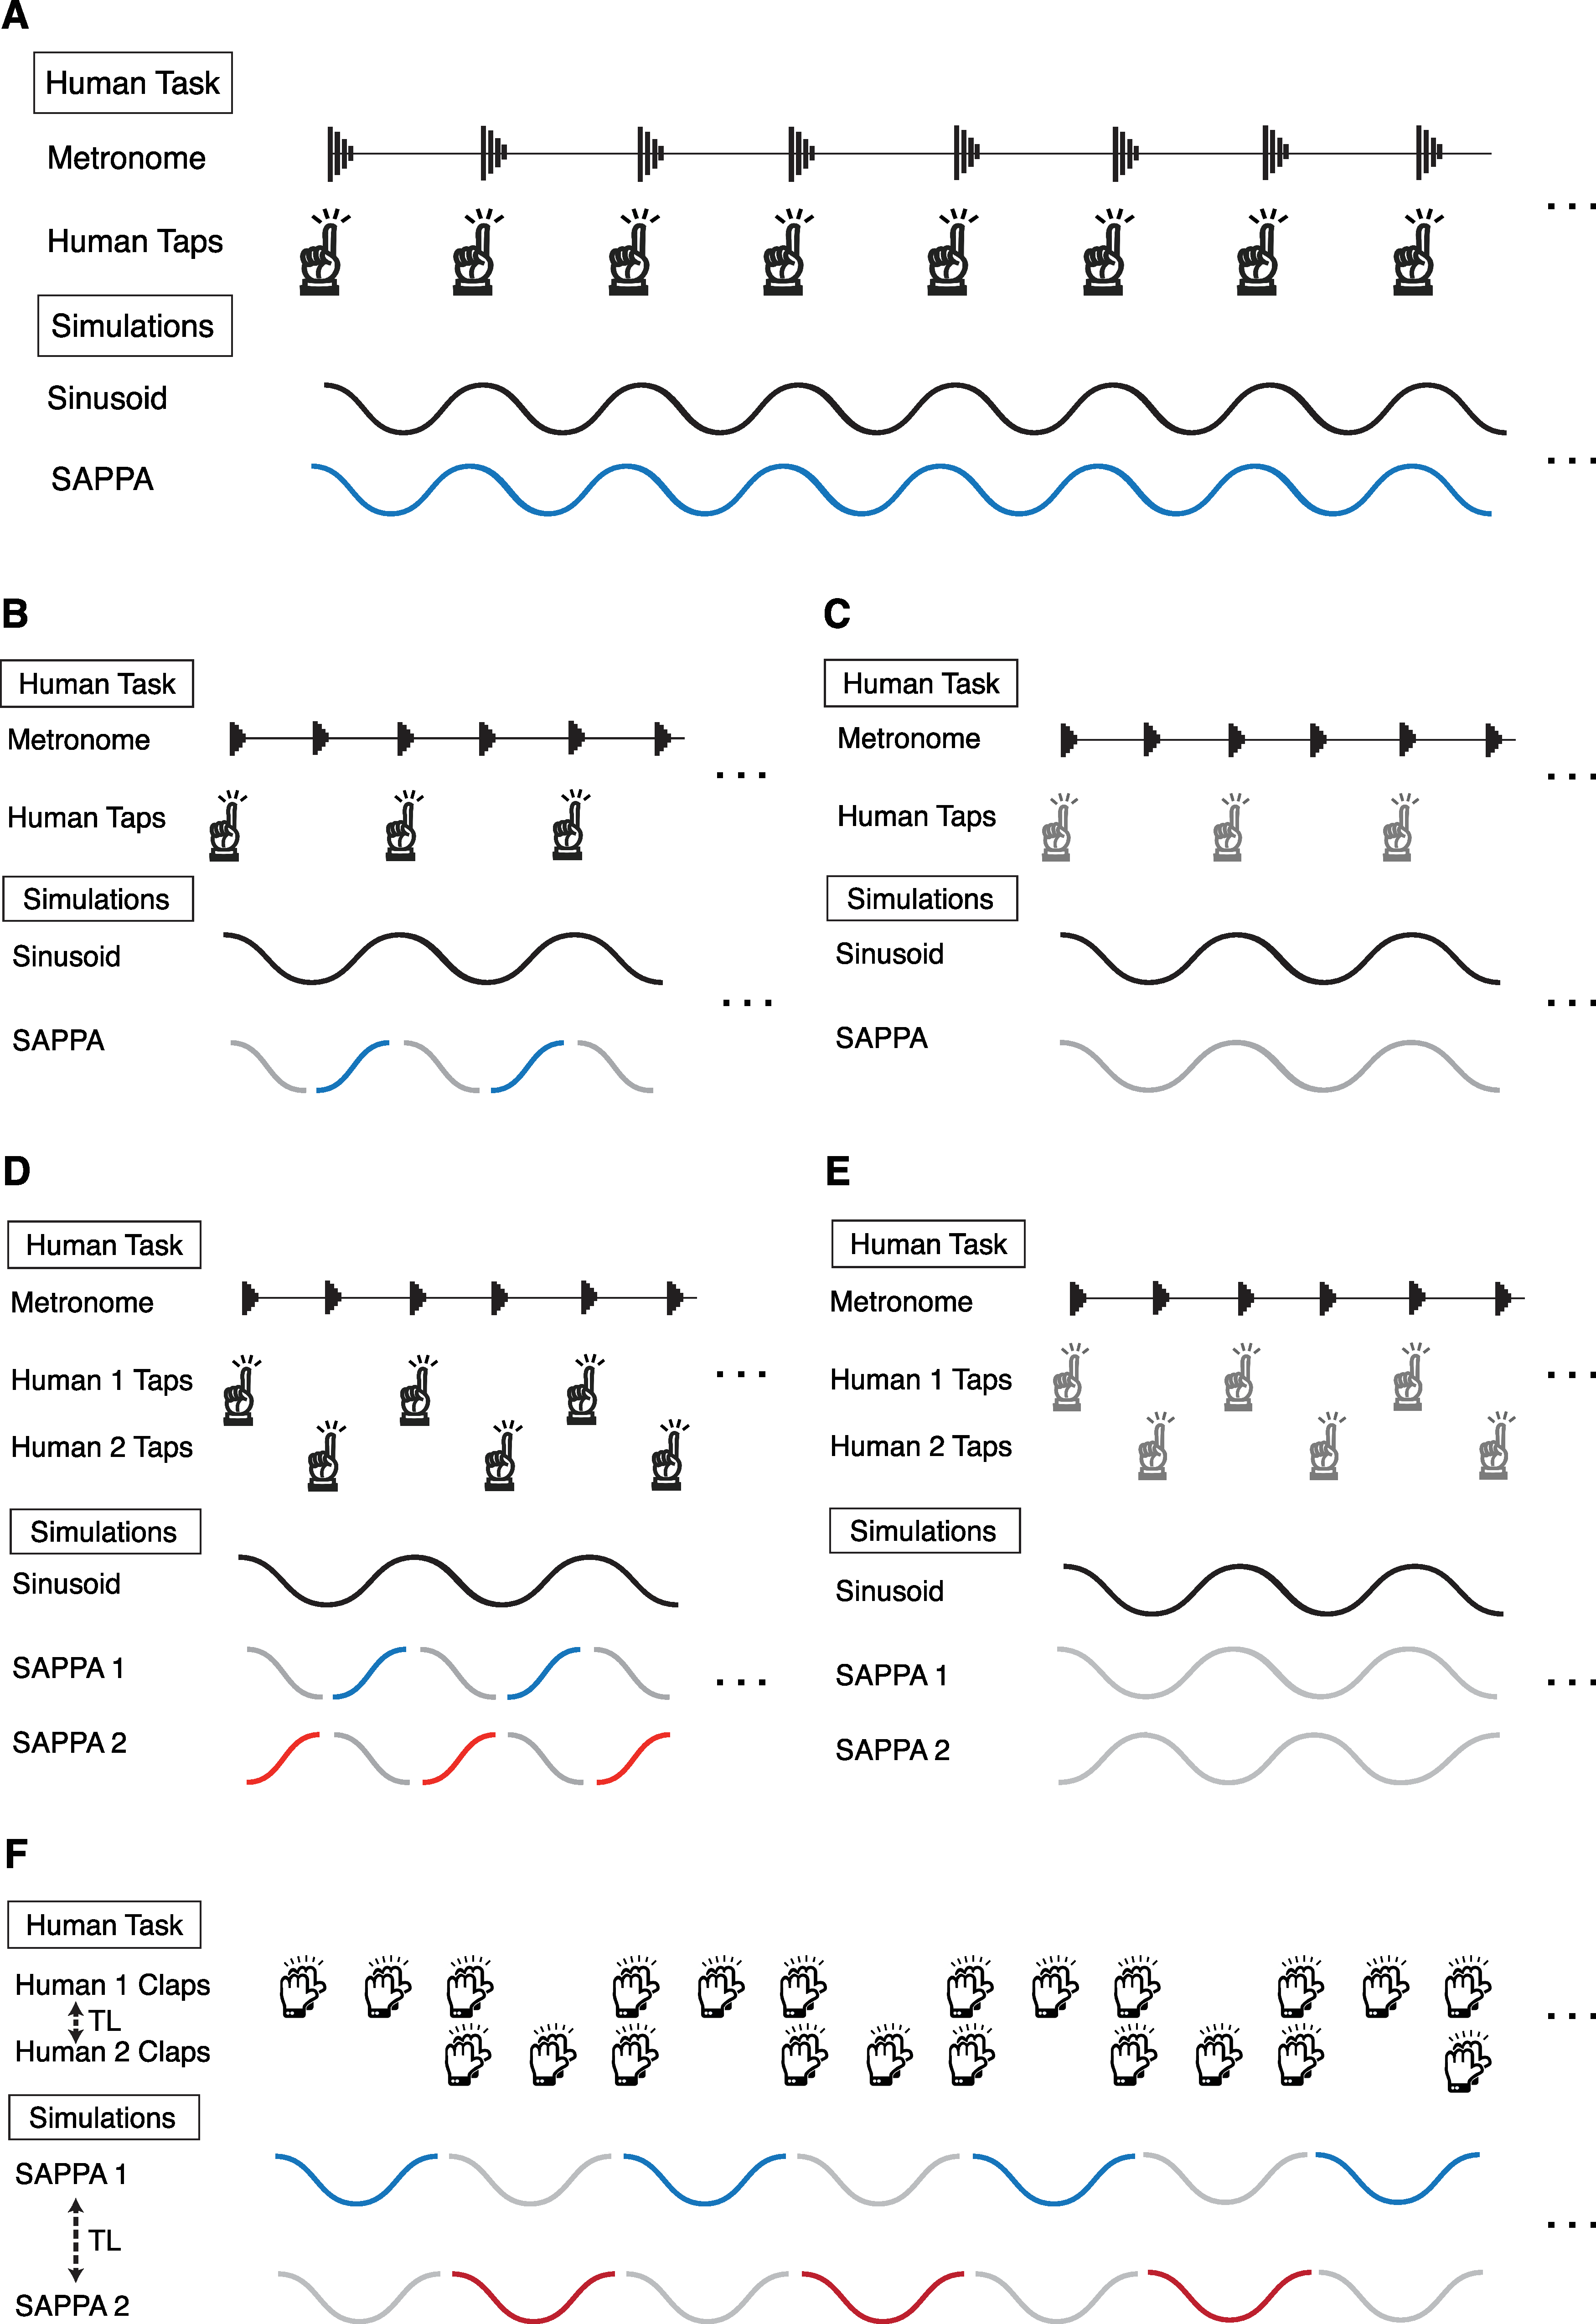
\includegraphics[width=0.9\textwidth]{figures/fig2_1.png}
    \label{f2_1}
\end{figure}
\begin{figure}[t]
    \caption[Illustration of the synchronization tasks and corresponding simulation experiments]{\textbf{Illustration of the synchronization tasks and corresponding simulation experiments.} (A) The task simulated in Experiment 1, in which a person synchronizes with a metronome (top). Illustration of our simulation, in which our model synchronizes with an external sinusoidal stimulus (bottom). (B) The first task simulated in Experiment 2, in which one musician taps to every other metronome beat while listening his or her own taps (top). Illustration of our simulation in which a SAPPA model synchronizes with an external sinusoidal stimulus (bottom). Blue colored part of the model's activity indicates that the model is receiving its own non-delayed activity as input in addition to the external sinusoid, and gray colored part indicates that the model only receives the external sinusoid as input. (C) The second task simulated in Experiment 2. This task is the same as the first one described in (B), except that the musician did not hear his or her own taps (top). Illustration of our corresponding simulation (bottom). The gray lines indicate that the model only receives the external sinusoid as input. (D) The third task simulated in Experiment 2, in which two musicians alternately tap with a metronome while listening to their own taps and the other musician's taps (top). Illustration of our simulation where two models synchronize with an external sinusoidal stimulus (bottom). Blue and red colored parts of the model's activity indicate the time window where the model's non-delayed activity is used as input for both models in addition to the external sinusoid, while grayed part indicates the time window when the model receives the non-delayed activity of the other model in addition to the external sinusoid as input. (E) The fourth task simulated in Experiment 2. This task is the same as the third one described in (D), except that the musicians did not hear their own or each other's taps (top). Illustration of our corresponding simulation (bottom). The grayed cycles indicate that the models only receive the external sinusoid as input. (F) The task simulated in Experiment 3, in which two musicians clapped a rhythm alternately (top). Illustration of our simulation where two models oscillate while alternately receiving each other's activity as input (bottom). Blue and red cycles indicate the model whose activity is received by both models as input, while gray cycles indicate that the model's activity is not received as input by either model. TL stands for transmission latency.}
\end{figure}

In our first experiment, we use the SAPPA model to reproduce the data from a study in which musicians and non-musicians synchronized their tapping with an isochronous metronome across a wide range of tempi, representing the simplest form of synchronization task \cite{repp2007tapping} (Fig.{} \ref{f2_1}A). Specifically, we hypothesize that the delayed recurrent feedback in the SAPPA model would result in an increasing anticipation tendency for the longer stimulus periods. Additionally, the smaller anticipatory tendency observed in musicians compared to non-musicians' anticipatory tendency would be achieved by reducing the amplitude of the delayed recurrent feedback.

In our second experiment, we reproduce the data from a study in which two musicians alternately tapped to a metronome \cite{nowicki2013mutual}. We are specifically interested in the data from two tasks where musicians tapped at every second metronome beat alone (Fig.{} \ref{f2_1}B and \ref{f2_1}C) or alternated this tapping with another musician as a duet (Fig.{} \ref{f2_1}D and \ref{f2_1}E). In both cases, their performance was measured in two conditions, with and without auditory feedback from tapping. The results show a smaller anticipatory tendency, in both solo and duet settings, when musicians heard their own taps compared to when they did not. We hypothesized that the lack or presence of non-delayed feedback in our model can simulate auditory feedback conditions, affecting the size of the anticipation.

In our third experiment, we reproduce behavioral data from duet performance with TLs (varying from 3ms to 78ms for different trials) where two musicians alternately clapped the same rhythmic pattern without a metronome \cite{chafe2010effect} (Fig.{} \ref{f2_1}F). Latencies longer than 20ms caused the musician starting the pattern to lag the musician finishing the pattern, while latencies shorter than 10ms caused the musician starting the pattern to clap ahead of the other musician's last clap. This resulted in the collective tempo gradually slowing down for the longer TLs and speeding up for the shorter ones. We hypothesized that our model's anticipation would be affected by longer TLs, resulting in lag between two synchronizing SAPPA models and a slowing tempo.

Perception-action coordination tasks capture how external and internal factors affect synchronization. The strong anticipation hypothesis explains synchronization with dynamical systems receiving external stimuli and delayed recurrent feedback. Our interest is to test whether a mathematical model of strong anticipation can be configured for solo and duet settings to perform a variety of synchronization tasks, and if so whether it could explain behavioral patterns observed in human data. This would demonstrate that the strong anticipation hypothesis accounts for complex biological phenomena like perception-action coordination.

\section{Results}

\subsection{Experiment 1: Individual tapping in synchronization with an \\ isochronous stimulus}

We simulated the model to represent an individual tapping with an isochronous stimulus (see Fig.{} \ref{f2_1}A), resulting in an anticipatory tendency. Fig.{} \ref{f2_2}A shows the linear regression we performed on the human data described by Repp and Doggett \cite{repp2007tapping}. We stimulated our model with a periodic external sinusoid and measured its anticipation (see model definition and parameter analysis in the methods section) with respect to the external sinusoid. In order to observe the relationship between anticipation and stimulus period length, we optimized our model parameters (see parameter analysis in the methods section) to simulate the anticipation shown by musicians and non-musicians, as a function of IOI \cite{repp2007tapping}. In Experiment 1, a single SAPPA model was stimulated by an external sinusoid while also receiving its own non-delayed activity as input. The range of oscillatory frequencies tested in Experiment 1 ranged from 0.29Hz to 1Hz (see the methods section for a full description of the model parameters and experimental conditions). This contrasted with Experiments 2 and 3, where the same model was stimulated differently, at a smaller set of frequencies.

\begin{figure}
    \centering
    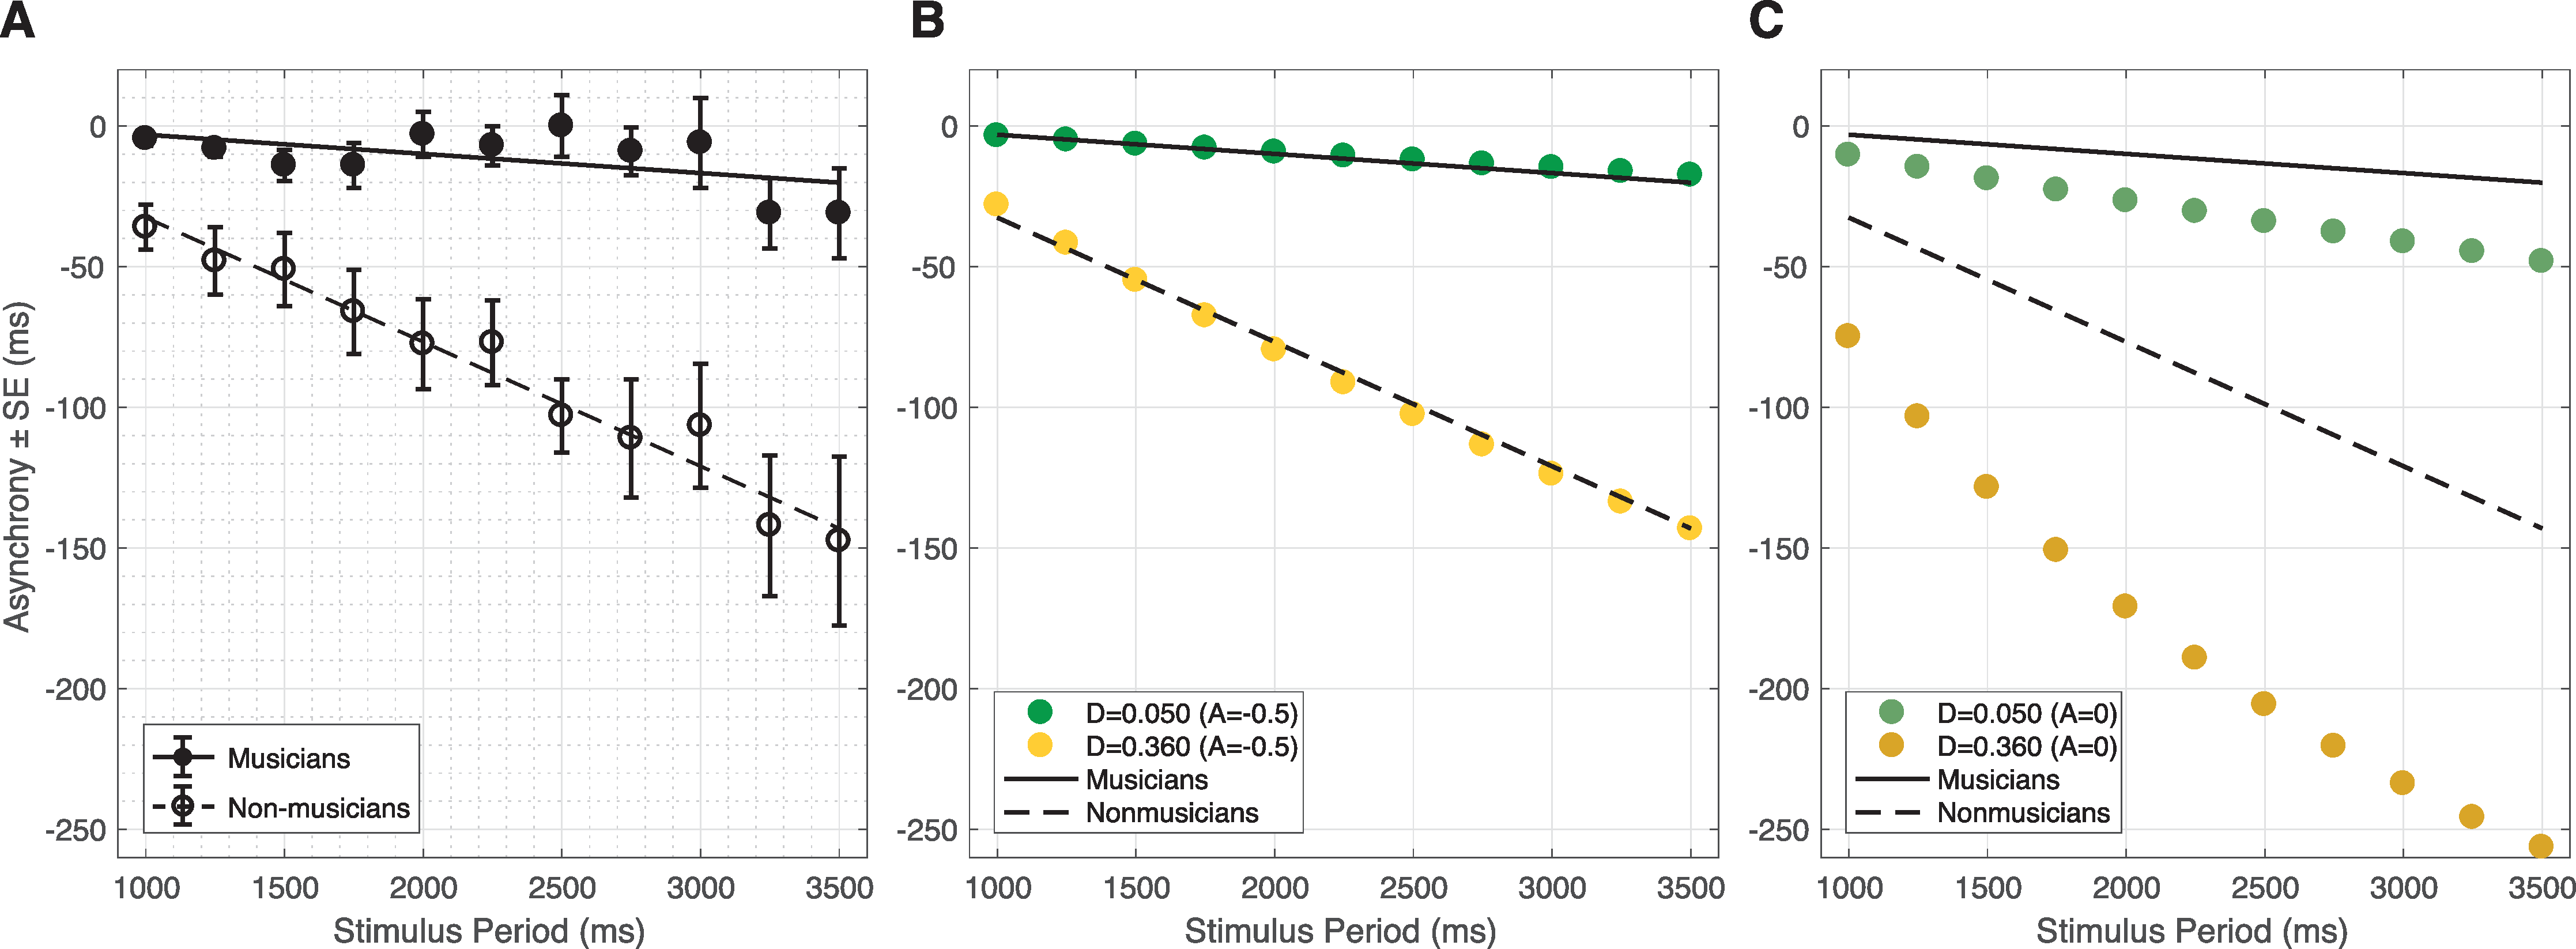
\includegraphics[width=1.0\textwidth]{figures/fig2_2.png}
    \caption[Dynamical systems model of anticipation when musicians and non-musicians synchronize with an isochronous stimulus]{\textbf{Dynamical systems model of anticipation when musicians and non-musicians synchronize with an isochronous stimulus.} (A) The anticipation (mean values with error bars representing the standard error of the mean) in musicians and non-musicians tapping with an isochronous metronome while listening their own taps. The regression lines for the mean values are also shown. (B) The anticipation obtained when the musician (green dots) and non-musician (yellow dots) SAPPA models were stimulated by an external sinusoid while also receiving their own non-delayed activity as input ($A = -0.5$; see model definition in the methods section). (C) The anticipation obtained when the musician (gray-green dots) and non-musician (gray-yellow dots) SAPPA models were only stimulated by an external sinusoid and did not receive their own non-delayed activity as input ($A = 0$; see model definition in the methods section). In all simulations $\tau = 0.222$ seconds. The $D$ parameter differentiates the musician and non-musician models. The same regression lines for the behavioral data are shown in both (A), (B) and (C) for comparison purposes (see Supplementary Fig.{} \ref{fS_1} for the model's behavior with a square wave input).}
    \label{f2_2}
\end{figure}

We ran our simulations for stimuli with periods of 1000, 1250, 1500, 1750, 2000, 2250, 2500, 2750, 3000, 3250, and 3500ms. The SAPPA model always had a recurrent feedback delay with length of 222ms. To simulate the musician and non-musician data, the SAPPA model had $D = 0.05$ and $D = 0.36$, respectively, where the parameter $D$ is the amplitude of the delayed recurrent feedback in the SAPPA model (see model definition and parameter analysis in the methods section). Using the same recurrent feedback delay length, we were able to make the slope of the anticipation, as a function of IOI, more negative by increasing the amplitude of $D$. Fig.{} \ref{f2_2}B shows how our simulated anticipatory tendencies align with the line of regression on the behavioral data for musicians and non-musicians in the study by Repp and Doggett \cite{repp2007tapping}. Fig.{} \ref{f2_2}C uses the SAPPA model to predict how behavioral data would look if musicians and non-musicians carried out the same task only listening to the metronome and not receiving auditory feedback about their taps. Under this condition, the SAPPA model predicts that the asynchrony in musicians and non-musicians would become more negative, compared to when they received auditory feedback about their taps.

In this simulation, the following parameters were used: $A = -0.5$ (non-delayed feedback amplitude), $\tau = 0.222$ seconds (delay length), and $D = 0.05$ and $D = 0.36$ (delayed feedback amplitude) for the musician and non-musician SAPPA models, respectively. The stimulating sinusoid had an amplitude of $1$, while $A = -0.5$. This means that the model was forced more strongly by the external sinusoidal stimulus than by its own activity and that the SAPPA model's phase-locking behavior was determined by the phase of the external sinusoid. Also, since recurrent feedback terms were negative ($A = -0.5$), the delayed recurrent feedback shifted the phase of $F$ in a negative direction with respect to $\exp(i2\pi f_s t)$. This means that the SAPPA model's actions were more aligned with $F = \frac{\exp(i2\pi f_s t)+Az}{|\exp(i2\pi f_s t)+Az|}$, thus resulting in reduced anticipation compared to when $F = \exp(i2\pi f_s t)$ (see the methods section for a thorough description of the model's dynamics, parameters, and discussion of how different model components interact with each other).

\subsection{Experiment 2: Interpersonal synchronization during alternating \\ paced tapping with or without auditory feedback}

Experiment 1 showed that our model can capture the anticipation observed in musicians and non-musicians in a simple metronome tapping task. Next, we examined how the SAPPA model could perform the more complex tasks in the study by Nowicki and colleagues \cite{nowicki2013mutual}. This task was carried out by solo musicians and also by musician duets. In the solo task, musicians tapped every other beat in synchrony with a metronome while hearing their own taps (feedback-on, Fig.{} \ref{f2_1}B) or only hearing the metronome (feedback-off, Fig.{} \ref{f2_1}C). In the duet task, pairs of musicians alternately tapped with a metronome while hearing their own and their partner's taps (feedback-on, Fig.{} \ref{f2_1}D) and also while only hearing the metronome (feedback-off, Fig.{} \ref{f2_1}E). The same model and parameters used in Experiment 1 were used in Experiment 2, except for the f term, which was varied in Experiment 1 but was always 1Hz in Experiment 2, matching the frequency of the stimulating external sinusoid. Another major difference was the way in which the model was stimulated. Similar to Experiment 1, each SAPPA model in Experiment 2 was constantly stimulated by an external sinusoid. However, in Experiment 2 in the solo condition with feedback-on, the model received its own non-delayed activity as input only during half of each cycle. Moreover, in Experiment 2 in the duet condition with feedback-on each model received its own non-delayed activity as input during one half of each cycle and the other model's non-delayed activity during the other half of the cycle. Finally, in Experiment 2 in the feedback-off condition, the models were only stimulated by the external sinusoid (see the methods section for a full description of the model parameters and experimental conditions).

Fig.{} \ref{f2_3}A shows that the anticipation exhibited by musicians when solo-tapping on every other beat to an isochronous metronome was larger without auditory feedback from their own taps. The results of our solo-tapping simulations for the musician and non-musician SAPPA models are illustrated in Fig.{} \ref{f2_3}B and \ref{f2_3}C, respectively (the SAPPA models used in this simulation have the same parameters found in Experiment 1; see the methods section for details about how we carried out this simulation of the solo task). We observed that the SAPPA model's anticipation was smaller when the model did receive its non-delayed activity as input, compared to when only receiving the external sinusoid as input. While no study has yet investigated non-musicians' asynchronies in this solo-tapping task, our non-musician SAPPA model predicts that non-musicians' asynchronies would be larger than musicians' asynchronies. Our SAPPA model also predicts that, similar to musicians, the non-musicians' asynchronies will be smaller when individuals can hear their own taps along with the metronome, compared to when they only hear the metronome.

\begin{figure}
    \centering
    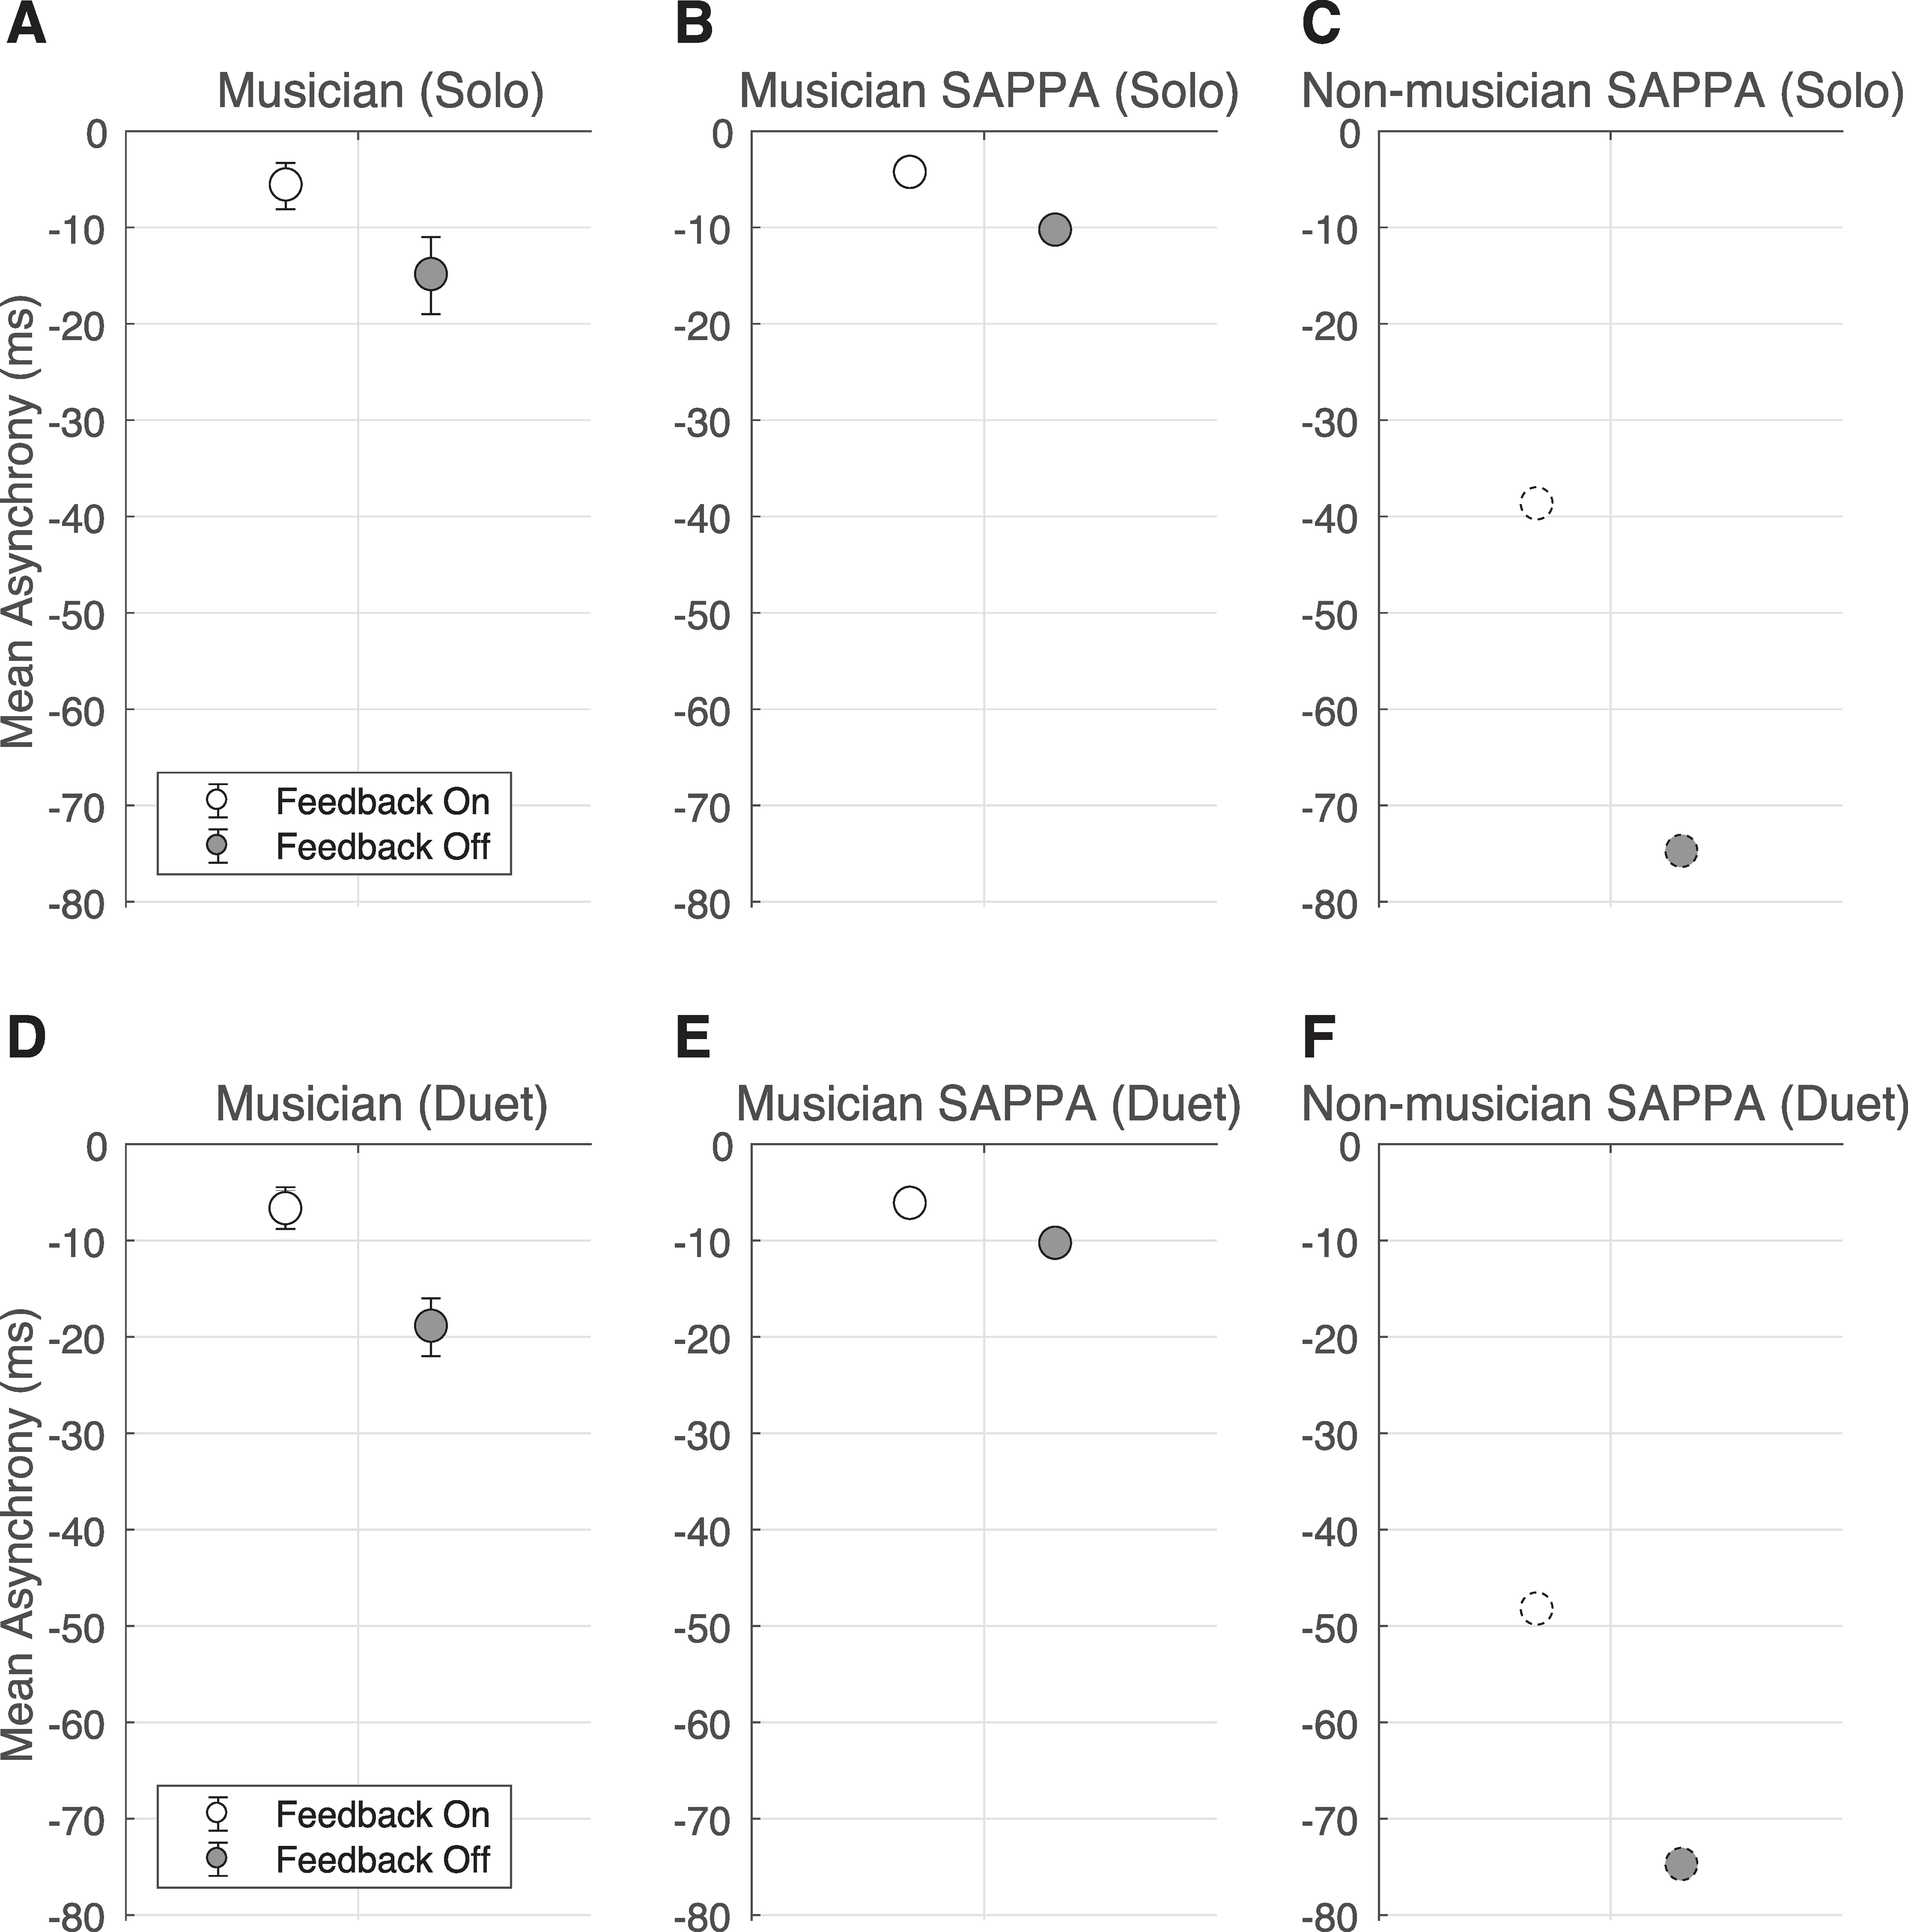
\includegraphics[width=0.8\textwidth]{figures/fig2_3.png}
    \caption[The effect of auditory feedback on anticipation when musicians synchronize with an isochronous metronome alone or with a musician partner]{\textbf{The effect of auditory feedback on anticipation when musicians synchronize with an isochronous metronome alone or with a musician partner.} (A) Behavioral measurements when a single musician taps every other beat in synchrony with a metronome for the feedback-on and feedback-off conditions (mean asynchronies with error bars representing the standard error of the mean). (B) The musician SAPPA model's anticipation when synchronizing with an external sinusoid, while receiving (feedback-on) or not receiving (feedback-off) its non-delayed activity as input every other beat. (C) The non-musician SAPPA model's anticipation when synchronizing with an external sinusoid, while receiving (feedback-on) or not receiving (feedback-off) its non-delayed activity as input every other beat. Dotted contours around circle data points indicate that this is a prediction that can be tested with behavioral data from non-musicians. (D) Behavioral measurements when two musicians tap every other beat in synchrony with a metronome for feedback-on and feedback-off conditions (mean asynchronies with error bars representing the standard error of the mean). (E) The anticipation when two musician SAPPA models synchronize with an external sinusoid, while alternating (feedback-on) or not receiving at all (feedback-off) each other's non-delayed activity as input every beat. (F) The anticipation when two non-musician SAPPA models synchronize with an external sinusoid, while alternating (feedback-on) or not receiving at all (feedback-off) each other's non-delayed activity as input every beat. Dotted borders around data points indicate that this is a prediction that can be tested by collecting behavioral data from non-musicians.}
    \label{f2_3}
\end{figure}

Fig.{} \ref{f2_1}D and \ref{f2_1}E show the duet behavioral task, which consists of two musicians tapping in alternation by each synchronizing with every other beat of an isochronous metronome. Fig.{} \ref{f2_3}D shows that, similar to the solo task results, the anticipation in musicians for the duet task was larger when they could not hear their own or their partner's actions. The results of our duet-task simulations with the musician and the non-musician SAPPA model are illustrated in Fig.{} \ref{f2_3}E and Fig.{} \ref{f2_3}F, respectively (the SAPPA models used in this simulation have the same parameters found in Experiment 1; see the methods section for details about how we carried out this simulation of the duet task). We observed that the SAPPA model's anticipation was smaller when models alternatingly received each other's non-delayed activity as input, compared to when they only received the external sinusoid as stimulus. No study has yet investigated non-musicians' asynchronies in this duet-tapping task, but we can use the non-musician SAPPA model to make predictions. Compared to anticipation in musicians, the SAPPA model predicts that anticipation in non-musicians would be larger. The SAPPA model also predicts that, similar to musicians, the non-musician anticipation will be smaller when pairs of individuals can hear each other's alternating taps along with the metronome, compared to when they only hear the metronome.

\subsection{Experiment 3: Interpersonal synchronization during rhythm-\\ clapping alternation in the presence of transmission latencies}

In Experiment 2 we coupled pairs of SAPPA models to simulate the flow of auditory information between partners performing a paced alternating tapping task. Here we conduct another simulation for the data described by Chafe and colleagues \cite{chafe2010effect}, by further extending our model and task configuration. Their study examined how TLs between duet partners affected synchronization while they alternately clapped a rhythmic pattern (see Fig.{} \ref{f2_1}F). The two novel features in their task were that they added TLs to the information exchange between duet partners who performed the task in two different rooms, and that they used a rhythmic pattern for alternating clapping instead of single-beat alternation. The same model and parameters used in Experiments 1 and 2 were used in Experiment 3. The main differences were, again, the way in which the model was stimulated and the oscillatory frequency. In contrast with Experiments 1 and 2, the SAPPA models in Experiment 3 were never stimulated by an external sinusoid. Instead, pairs of oscillators ($f = 1.5$Hz) stimulated each other in an alternating fashion every cycle (see the methods section for a full description of the model parameters and experimental conditions).

In the results by Chafe et al. \cite{chafe2010effect}, for TLs smaller than 10ms, the musician starting their rhythm showed a tendency to slightly lead the musician finishing a turn. With TLs greater than 10ms, the musician starting their turn lagged the musician finishing a turn. A similar pattern of behavior was observed as a result of TLs between the two oscillators. Fig.{} \ref{f2_4}A illustrates our simulations with two oscillators that alternated cycles based on which oscillator served as the `active' one. The colored background indicates the oscillator whose activity was used as the input for both oscillators (see the methods section for more details about how we carried out this simulation). In the example shown in Fig.{} \ref{f2_4}A, the oscillator initiating its active cycle tended to lag the endpoint of the other oscillator as a result of the TL. In human data, these asynchrony measures grew as a function of TL, as shown in Fig.{} \ref{f2_4}B. Fig.{} \ref{f2_4}C and \ref{f2_4}D show our simulations with musician and non-musician SAPPA models, respectively, where the lag between coupled models showed a growth similar to the one observed in the behavioral study. The main difference between the behavioral data (Fig.{} \ref{f2_4}B) and our simulations (Fig.{} \ref{f2_4}C and \ref{f2_4}D) is that in our simulations TLs smaller than 10ms did not result in positive values. No existing studies have addressed how non-musicians perform in this task. Our non-musician SAPPA model predicts that, compared to musicians, the effect of TLs on non-musician synchronization behavior will be similar to that observed for musicians, indicating that TLs consistently affect synchronization between two clapping individuals, independent of musical expertise.

\begin{figure}
    \centering
    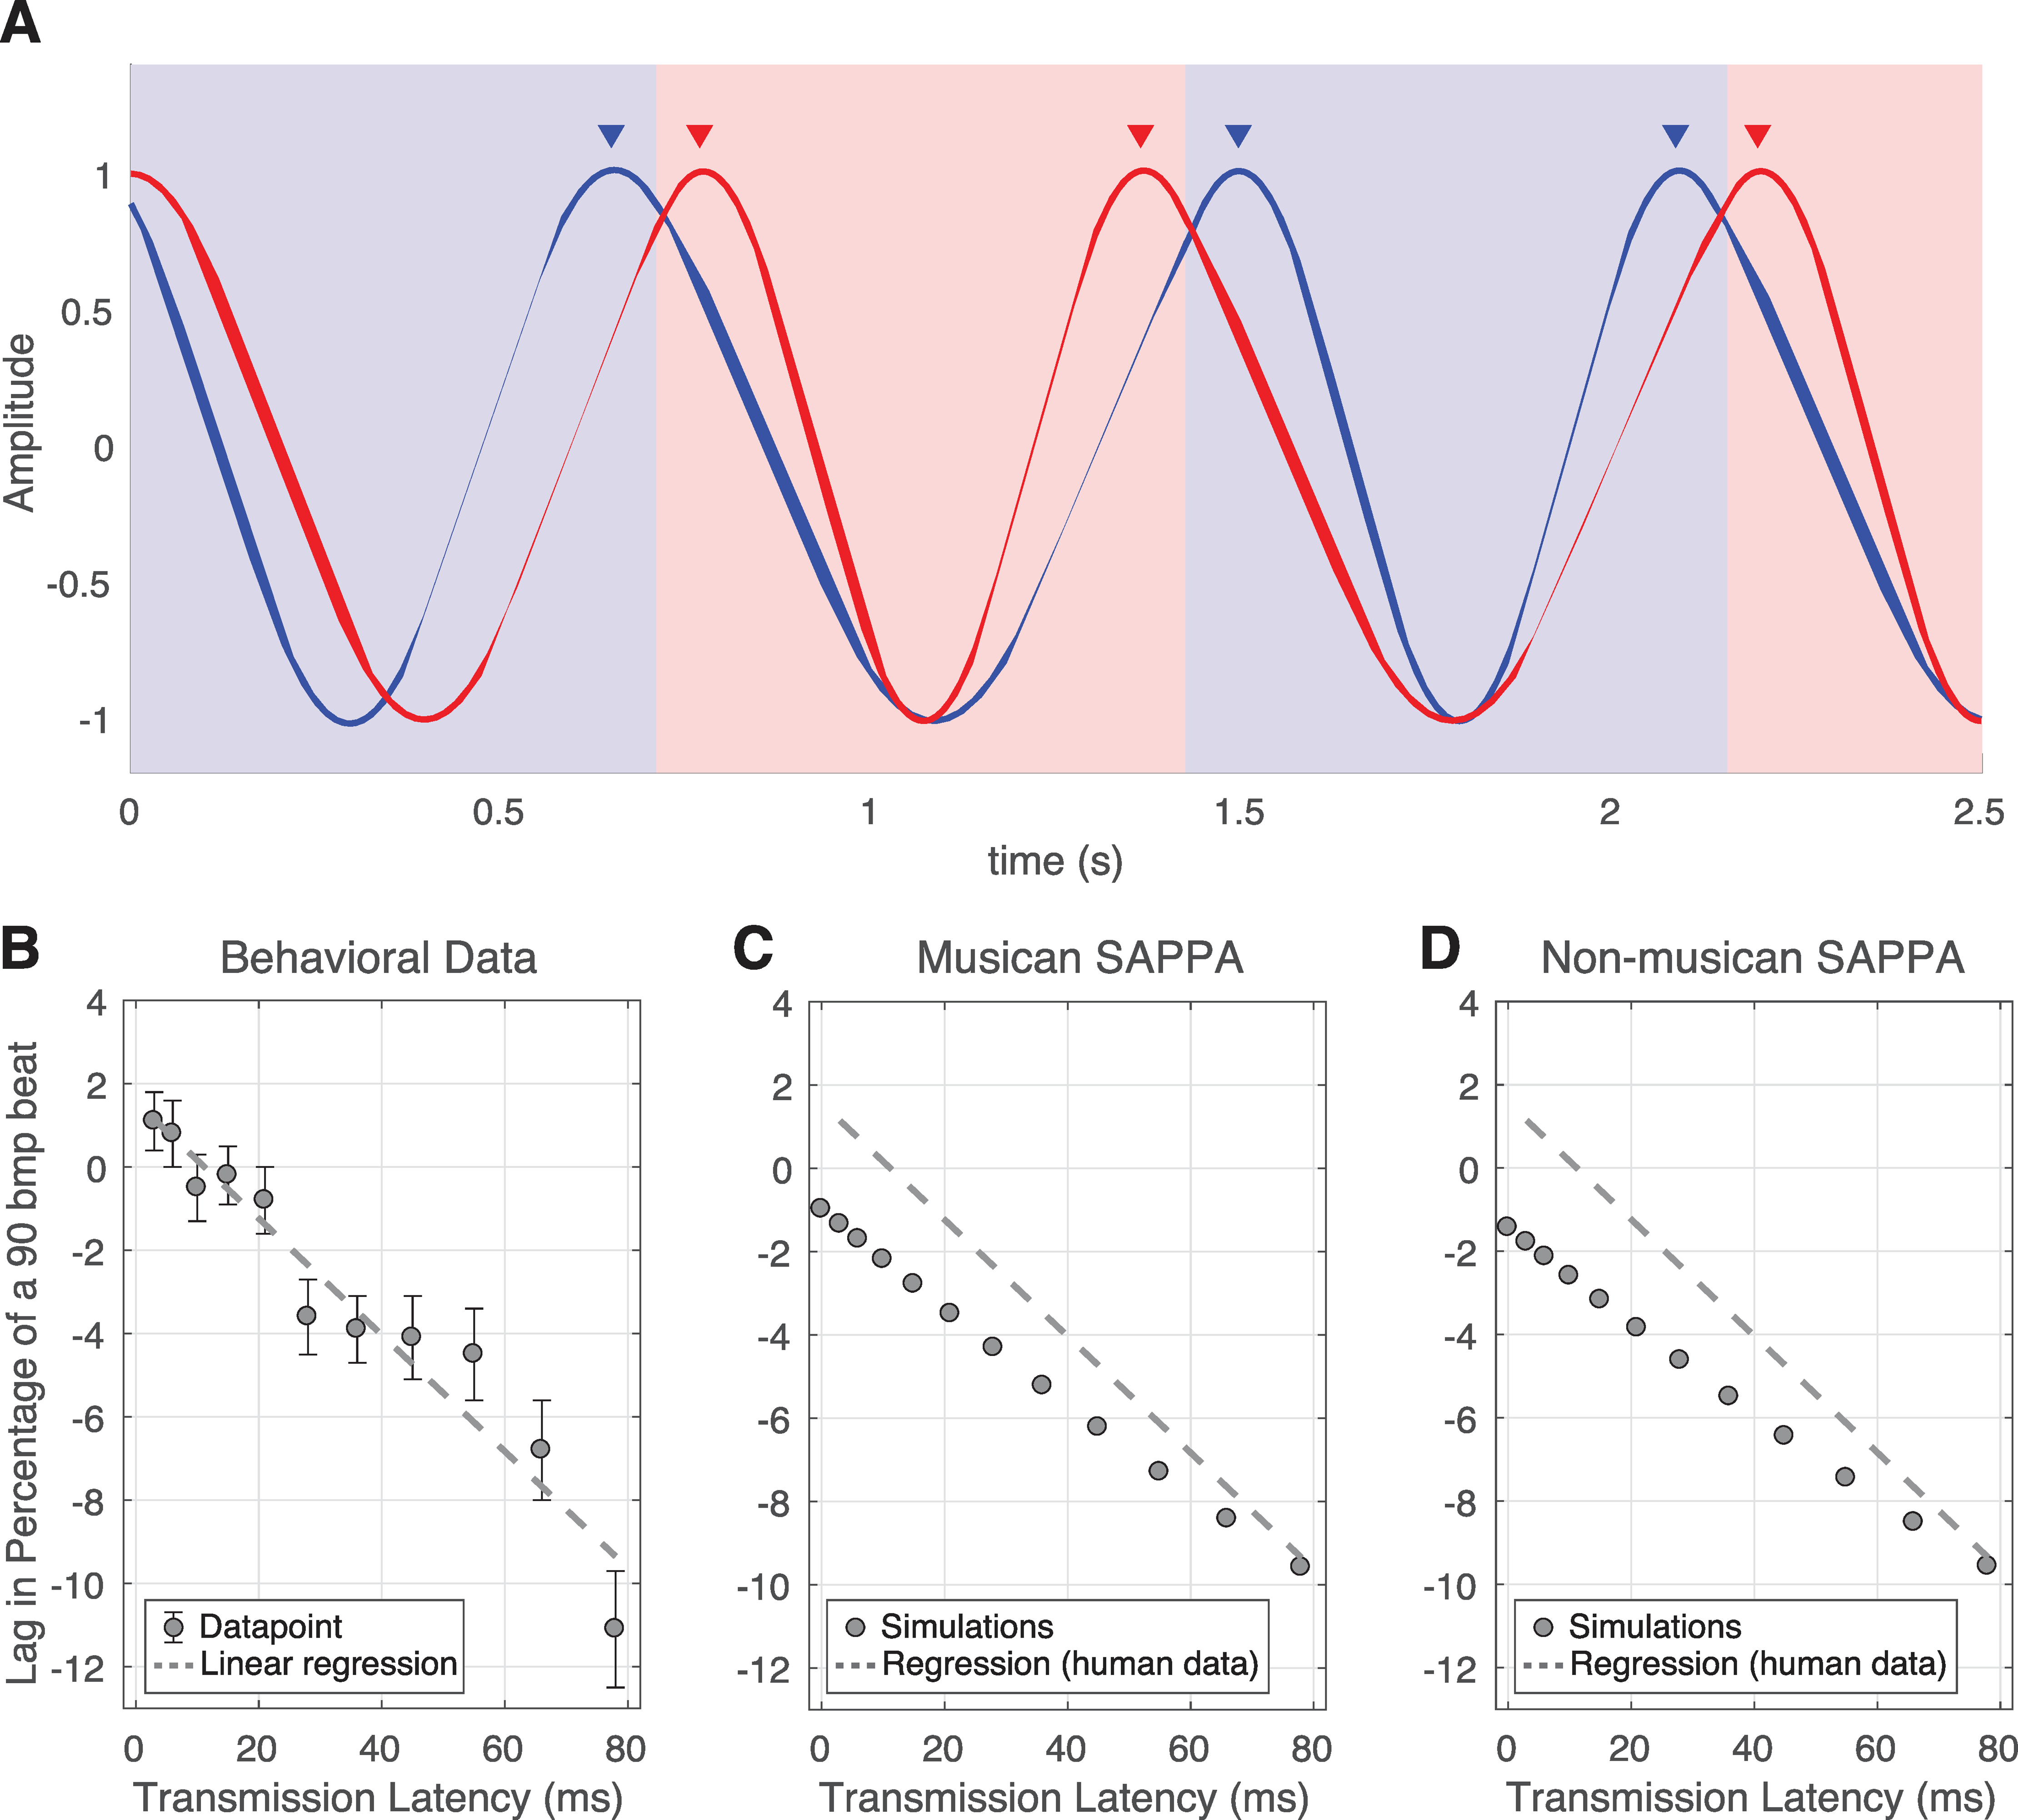
\includegraphics[width=1.0\textwidth]{figures/fig2_4.png}
    \caption[The effect of transmission latencies on the anticipation of pairs of musicians alternatively clapping a rhythm]{\textbf{The effect of transmission latencies on the anticipation of pairs of musicians alternatively clapping a rhythm.} (A) Illustration of the dynamics observed during our simulations in the presence of a TL between two synchronizing SAPPA models. The alternating blue and red background colors indicate which model's activity is used as input to both models. The arrows show the end points of cycles for both models. Note how the passive model lags the active model in turn at the end of the cycle, due to the presence of the TL. (B) The lead and lag between musicians (measured as the percentage of a 90 bpm beat) as a function of TLs (mean values with error bars representing the 95\% variance), with the linear regression on the behavioral data. (C-D) The lead and lag between pairs of musician (C) and non-musician (D) models, with the linear regression from the behavioral data (B) for comparison purposes.} 
    \label{f2_4}
\end{figure}

\section{Discussion}

\subsection{Delayed recurrent feedback results in anticipatory \\ tendencies during paced periodic action}

Our model shows that asynchronies become smaller when the length of the recurrent feedback delay is shortened (see parameter analysis in the methods section). This is a result of the fact that $z$ and $z(t—\tau)$ become maximally aligned as $\tau$ shrinks. Consistent with the observations by Ciszak and colleagues \cite{ciszak2004dynamical}, our simulations show that the phase difference between $z$ and $z(t—\tau)$ is what causes anticipatory behavior. This behavior is similar across different types of external periodic inputs (for example, see Supplementary Fig.{} \ref{fS_1} for the model's behavior when the external input is a square wave instead of a sinusoid). It is interesting to consider whether the observed phase difference between $z$ and $z(t—\tau)$ is similar to the communication delays that exist in the physiology of the sensorimotor system. In principle, today's imaging techniques can support the quantification of actual conduction delays between neurons located in the auditory cortex, the basal nuclei, the cerebellum, premotor and motor cortex, as well as extremities and effectors (e.g., fingers). For example, high resolution neuroimaging methods and the physical models of axonal conduction delays may allow for the estimation of these delays through integration over populations \cite{swadlow2012axonal}. However, these areas contain vast numbers of neuronal connections which likely differ from each other in their functional pathways. Thus, detailed estimation of these delays at microscopic levels may not easily translate to macroscopic representation of neuronal population behaviors. Given that the recurrent feedback delay length is arbitrarily set in our model, the recurrent feedback delay length described here should be considered a representation of the potential function of neural transmission delays in a collective fashion.

\subsection{Experiment 1: Individual tapping in synchronization with an \\ isochronous stimulus}

In the SAPPA model Eq \eqref{eq:2.5}, a larger $D$ increases the amplitude of the delayed recurrent feedback. These different amplitudes have an effect on the anticipatory mechanisms of the model. $D$ is divided by the frequency $f$ in Hz. As $f$ becomes smaller, $\frac{D}{f}$ becomes exponentially larger. Hence, the delayed recurrent feedback is amplified as a function of the stimulus interval, which in turn results in the growing anticipation. Physiologically, this means that the $\frac{D}{f}$ parameter could indicate the amplitude of neural activity that one processes in addition to the external stimulus. This amplitude becomes larger as the stimulus becomes slower.

Our model was able to reproduce the mean anticipatory dynamics of musicians and non-musicians tapping with IOI periods between 1000ms and 3500ms. This was due to the smaller $D$ that made the musician SAPPA model anticipation curve have a less negative slope as a function of stimulus period length, compared to the larger $D$ that resulted in a more negative slope of non-musician SAPPA model. Since the amplitude of the delayed recurrent feedback in the non-musician SAPPA model is overall larger compared to the musician SAPPA model, $\frac{D}{f}$ makes the delayed recurrent feedback grow more in amplitude as a function of longer stimulus period. As discussed above, directly relating this $D$ parameter to the real neural processes might be difficult because it captures the cumulative effect of multiple interacting neural delay processes \cite{van2003self}. What we can say is that the larger $D$ value in the non-musician model causes larger amplitudes in the oscillators compared to the musician model.

We assumed that a linear regression on the behavioral data could fairly characterize the anticipatory dynamics observed in musician and non-musician data (Fig.{} \ref{f2_2}A). This assumption is a limitation: anticipatory timing does not grow indefinitely as a function of IOI. Experiments where humans synchronize taps with a metronome of IOIs longer than 3500ms show that some taps precede the stimulus while others follow it, reducing the mean asynchrony \cite{baaaath2016estimating}, or even showing mean positive asynchronies for IOIs greater than 5000ms \cite{miyake2004two}. Hence, the relationship between metronome IOI and human asynchronies are non-linear. Non-linearities are a common feature in non-linear systems with delayed recurrent feedback \cite{khalil2002nonlinear}. As a result, our model's behavior is non-linear, a feature that is more visible in our simulation of non-musician anticipation than musician anticipation (Fig.{} \ref{f2_2}B and \ref{f2_2}C). These non-linear features could be used to expand the SAPPA model by making it show positive asynchronies in simple tapping tasks, like people do when stimulated by IOIs greater than 5000ms \cite{miyake2004two}. Because of these non-linear features, the SAPPA model has potential to explain both positive and negative asynchronies observed when people tap with metronomes of different IOI lengths.

Behavioral studies have consistently shown that anticipation when tapping with a metronome differs between musicians and non-musicians \cite{mates1994temporal, repp2007tapping, miyake2004two}. Our model offers an explanation as to what underlying mechanisms could give rise to these differences. Here, only the $D$ parameter was different between our musician and non-musician models, with $D$ being smaller in the musician model. Moreover, the simulation in Fig.{} \ref{f2_2}C predicts that the anticipation will be larger for both musicians and non-musicians synchronizing with a metronome without listening their own taps, compared to when they listened their own taps (Fig.{} \ref{f2_2}A and simulation in Fig.{} \ref{f2_2}B). This prediction made by the SAPPA model could be tested by collecting empirical evidence from musicians and non-musicians. Furthermore, by changing its parameters, our model allows us to make even more predictions, beyond the ones made in Fig.{} \ref{f2_2}C.

Compared to the musician model, the larger $D$ parameter in the non-musician model could be equivalent to a scenario where non-musicians listen to their internal processes more than musicians. In other words, in the non-musician's brain the strength of internal feedback is larger compared to the musician's brain, resulting in processing of an internal signal in addition to processing of external stimuli or behavioral adjustments. In this analysis we focused on the $D$ parameter, but the $\beta$ parameter in the SAPPA model would have had a similar effect (see model definition in the methods section for a full description of the model parameters). Electrophysiological findings from investigations on cortical oscillatory amplitude support this observation. Compared to resting conditions, non-musicians listening to music show larger oscillatory amplitudes only in the delta band (between 0.5Hz and 4Hz) \cite{bhattacharya2005phase}, which overlaps with the frequency range of stimuli tested in our Experiment 1. In contrast, musicians listening to music show synchrony in a more diverse set of neural oscillation frequencies, including delta and gamma (greater than 30Hz) bands \cite{bhattacharya2005phase}. Our model's $D$ parameter could be inversely proportional to the number of neural oscillation frequency bands observed when listening to music compared to resting conditions. Other neuroscientific research regarding the question of how musical expertise affects synchronization indicates that, compared to non-musicians, musicians show enhanced executive function and activation of the supplementary motor area \cite{zuk2014behavioral}, are better able to imitate hand gestures \cite{spilka2010gesture}, and show greater connectivity between premotor and striatal brain areas during beat perception \cite{grahn2009feeling}. Hence, musical expertise affects synchronization. Further, Riley and colleagues \cite{riley2012learning} hypothesize that behaviors involving precision, like perception-action coordination, rely on synergy formation, which is associated with a reduction of the degrees of freedom that a person has to handle cognitively during a task. Through training, synergies associated with synchronization may be greater in musicians than in non-musicians. The $D$ parameter in the SAPPA model could be understood as related to the number of degrees of freedom that a person has to handle during perception-action coordination, since $D$ had a smaller value in the musician SAPPA model compared to the non-musician SAPPA model.

Our model lacks variability in its behavior when synchronizing with an isochronous stimulus. When people tap with an isochronous stimulus, a mean negative asynchrony is observed with a large variability around it \cite{repp2005sensorimotor}. This means that some people may exhibit mean positive asynchronies (e.g., reaction to the stimulus rather than anticipating). The current SAPPA model can only describe the mean anticipatory tendency observed when averaging data across individuals. Variability in the SAPPA model could be achieved with simulations where the $D$ parameter is varied using a gaussian distribution centered around the $D$ values we found for musicians and non-musicians. B\aa\aa th \cite{baaaath2016estimating} used mixed gaussian distributions to simulate the anticipation variability seen in the behavioral experiments similar to those in Repp and Doggett \cite{repp2007tapping}. Using gaussian distributions to add variability to the SAPPA model would also allow models of individual participants to have different parameters. One could test whether the SAPPA model's $D$ parameter is related to individual's oscillatory power or years of musical training. The SAPPA model is currently unable to explain anticipatory tendencies or positive asynchronies observed outside the IOI range between 1000ms and 3500ms. Future investigations should test the SAPPA model for anticipation outside the IOI range we investigated in this study. When tapping with IOIs longer than 3500ms, people may show mean positive asynchronies, while mean negative asynchronies are observed when tapping with IOI lengths shorter than 1000ms \cite{miyake2004two}. We already discussed in the previous paragraphs that the SAPPA model's non-linearities could explain the positive asynchronies observed for IOIs longer than 3500ms. Although beyond the scope of the current investigations, we did observe that for IOIs shorter than 1000ms, the SAPPA model shows a negative asynchrony, consistent with behavioral data.

\subsection{Experiment 2: Interpersonal synchronization during alternating \\ paced tapping with or without auditory feedback}

In the solo and duet conditions, our musician SAPPA model showed less anticipation when musicians tap every other metronome beat hearing their own actions compared to when only hearing a metronome. When the SAPPA model synchronizes with its own non-delayed activity in addition to the external sinusoid, the input $F = \frac{\exp(i2\pi f_s t)+Az}{|\exp(i2\pi f_s t)+Az|}$ is the sum (as shown by Eq \eqref{eq:2.7} in model definition in the methods section). The smaller anticipation when as opposed to when $F = \exp(i2\pi f_s t)$ (i.e., only the external sinusoid) is caused by the instantaneous phase shift that $F$ suffers when $z$ gets subtracted from the external sinusoid $\exp(i2\pi f_s t)$, causing $F$ and $z$ to be more phase-aligned. In contrast, when only synchronizing with an external sinusoid, the delayed recurrent feedback $\frac{D}{f}z(t-\tau)$ (see Eq \eqref{eq:2.5} in model definition in the methods section) linearly adds with $F = \exp(i2\pi f_s t)$, resulting in a delayed phase shift, causing $F$ and $z$ to be less phase-aligned.

We simulated anticipation using the musician and the non-musician SAPPA models. As shown in Fig.{} \ref{f2_3}, the musician SAPPA model was able to show smaller anticipation in the feedback-on compared to the feedback-off condition in both solo and duet tasks. While the task by Nowicki and colleagues \cite{nowicki2013mutual} has not yet been tested with non-musicians, our simulations predict that the non-musician anticipation will generally be larger than the musician anticipation observed across tasks and conditions. We speculate that this prediction is highly likely, because it has been previously reported that non-musicians' asynchronies are larger than musicians' asynchronies \cite{repp2007tapping}. By collecting data from non-musicians carrying out this task one could test the validity of our model's predicted behavior.

Currently, the SAPPA model does not include modules that represent variabilities over time across individuals in a sample population. This means that it is limited in its ability to explain long-range temporal dynamics. Hence, anticipatory dynamics are limited to a local time scale. Incorporating noise in our model is beyond the scope of the work we present here, because the nature of noise as well as its sources and mechanisms remain largely unknown. As previously discussed, B\aa\aa th \cite{baaaath2016estimating} has modeled the noise associated with anticipation in the simplest metronome tapping task using a mixed gaussian distribution. To our knowledge, no studies have demonstrated how neural mechanisms and their intrinsic noise might be related to synchronization phenomena and anticipation. Variations in the environment and task requirements are also likely to add different types of noise that influence the overall system behavior. To effectively simulate different noise sources, it would be necessary to first study the distributions and mechanisms underlying variability in human adaptive behavior, using a large corpus of empirical data. Additionally, when quantifying how noise affects synchronization at local and global time scales, researchers should carefully consider that asynchronies tend to fluctuate on long-range time scales, which can affect the interpretation of behavioral data analysis and computational models \cite{torre2008distinct}.

Because the two musicians in the duet task tapped every other beat in alternation, the resulting interpersonal synchronization was anti-phase. Recent studies have used the Haken-Kelso-Bunz (HKB) model \cite{haken1985theoretical} (further discussed in the general discussion subsection below) to explain anti-phase interpersonal synchronization \cite{duarte2012interpersonal, dumas2014human, kelso2009virtual}. The SAPPA model and the HKB models are both able to explain anti-phase synchronization and anticipation at different phase relationships. Future investigations could analyze similarities and differences between these models when they synchronize with external periodic stimuli.

\subsection{Experiment 3: Interpersonal synchronization during rhythm-\\ clapping alternation in the presence of transmission latencies}

In the simulations in Experiment 3, two types of delay affected synchronization dynamics between coupled dynamical systems. The first one existed in the SAPPA model, as self-referential recurrent feedback delay in Eq \eqref{eq:2.5}, which resulted in anticipation (see model definition and parameter analysis in the methods section). The second one, TL, was introduced as the external informational delay in the communication between two oscillators, which is extrinsic to Eq \eqref{eq:2.5}. Our simulations integrate these two separate delays to explain how internal and external feedback in our model affect synchronization. Experiment 1 results showed that the first delay resulted in the anticipation, while the second delay can cancel the anticipatory behavior, resulting in disrupted synchronization. Our simulation results show that TLs similarly affected the synchronization of the musician and non-musician SAPPA models (Fig.{} \ref{f2_4}C and \ref{f2_4}D). This suggests that TLs affect synchronization independent of musical expertise. Future experiments can test our model's prediction of non-musician behavior by collecting data when non-musicians carry out the task introduced by Chafe and colleagues \cite{chafe2010effect}.

In Experiment 3, pairs of oscillators ($f = 1.5$Hz) stimulated each other in an alternating fashion every cycle. There was no external sinusoid stimulating the oscillators in this experiment (see setup, procedures and measurements in the methods section for a complete description). One caveat to our current model, is the fact that it cannot explain the positive values observed in existing human behavioral data (Fig.{} \ref{f2_4}C and \ref{f2_4}D). In the experiment by Chafe and colleagues \cite{chafe2010effect}, pairs of participants synchronized in the absence of the natural TL over air (due to wearing headphones), and in the presence of artificial TLs of fixed length. In the real world, synchronizing individuals have to always cope, at least, with the TL associated with sound travelling in air. We speculate that humans cope with such TLs by overestimating the frequency of their actions (i.e., a faster frequency), to make their actions reach the other participant on time. In the experiment by Chafe and colleagues \cite{chafe2010effect}, when neither air-travelling sound TL nor artificial TL existed, participants actions anticipated each other. The anticipation, indicated by positive values in the behavioral data in Fig.{} \ref{f2_4}B, is likely caused by musicians' expectation of the TL implicit in the transmission of sound in air, which is effectively removed when the TL is very small (<10ms). Our model is naive to the TL of sound travelling in air, and thus it was not affected in the same way by TLs smaller than 10ms. In the SAPPA model, the relationship between TL and the natural frequency of the oscillator can only be achieved by adding a bias that makes the SAPPA model complete its cycles before the driving stimulus (another SAPPA model in Experiment 3) completes a cycle. The $f$ term, which is a constant dictating the natural frequency of the SAPPA model's oscillatory behavior in units of hertz (see Eq \eqref{eq:2.5} in the model definition in the methods section), can be altered to explain the positive values in Fig.{} \ref{f2_4}B:  

\begin{equation}
\hat{f} = f + \triangle \label{eq:2.1}
\end{equation}

Here, in Eq \eqref{eq:2.1}, a positive offset $\triangle$ (positive real value bias) can be added to compensate for the effect of the transmission of sound through air. This $\triangle$ term would make the SAPPA model's frequency term slightly faster compared to the external stimulus, resulting in the positive values observed in Fig.{} \ref{f2_4}B for TLs smaller than 10ms. Fig.{} \ref{f2_5} shows our model's resulting behavior when $f$ is modified as described in Eq \eqref{eq:2.1}.

\begin{figure}
    \centering
    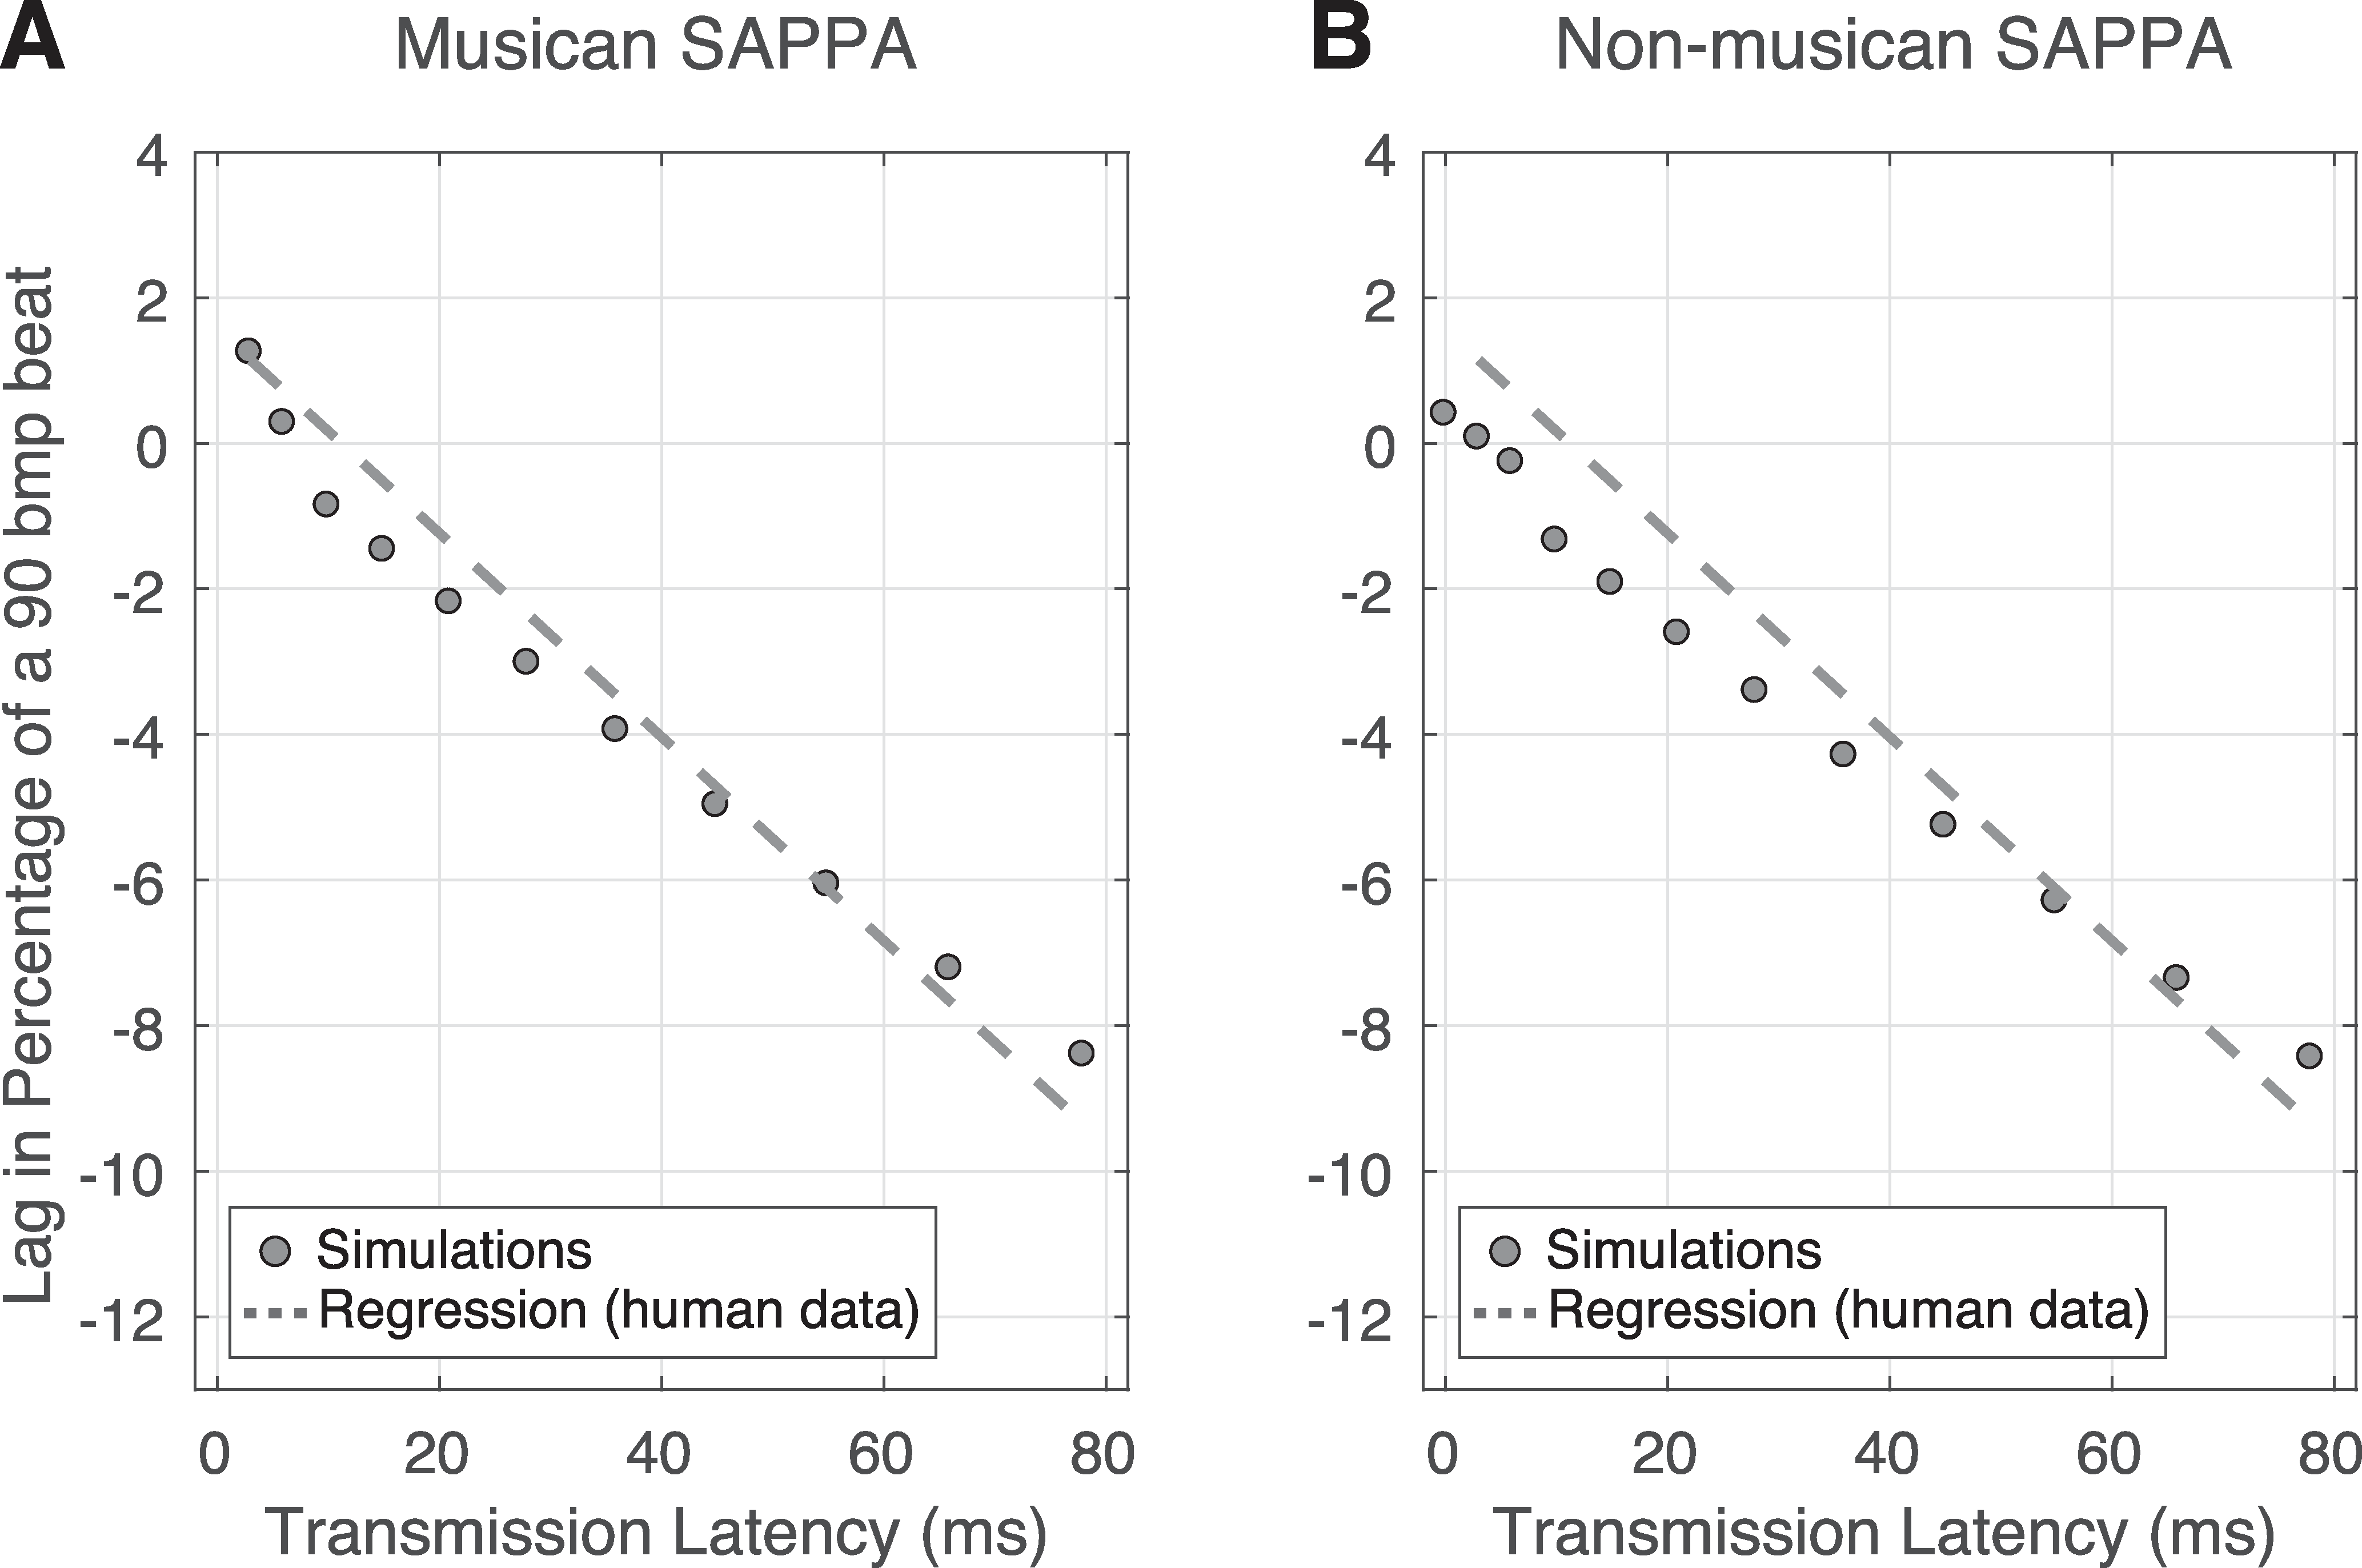
\includegraphics[width=1.0\textwidth]{figures/fig2_5.png}
    \caption[The effect of modified $f$ (Eq \eqref{eq:2.1}) on our model's simulation in Experiment 3 where pairs of musicians alternatively clap a rhythm in the presence of transmission latencies]{\textbf{The effect of modified $f$ (Eq \eqref{eq:2.1}) on our model's simulation in Experiment 3 where pairs of musicians alternatively clap a rhythm in the presence of transmission latencies.} The lead and lag between pairs of musician (A) and non-musician (B) models, measured as the percentage of a 90 bpm beat as a function of TLs, with $f$ modified as described in Eq \eqref{eq:2.1}. The linear regression on the behavioral data from Fig.{} \ref{f2_4}B is shown for comparison purposes.} 
    \label{f2_5}
\end{figure}

The behavior in Fig.{} \ref{f2_5} is the result of the frequency detuning introduced in Eq \eqref{eq:2.1}. Previous studies show that frequency detuning and delayed coupling between synchronizing HKB systems (see the General discussion below for more information about the HKB model) result in anti-phase solutions that are less stable than in-phase activity \cite{slowinski2016effects, avitabile2016beyond}. The behavioral data by Chafe and colleagues \cite{chafe2010effect} supports these observations, since musicians performed the same clapping rhythm in-phase, in an alternating fashion. As the transmission delay grew, in-phase synchronization became harder for pairs of synchronizing musicians. To cope with different TL lengths, musicians had to re-adjust the frequency of their actions every cycle to continue in-phase, but very long TLs made in-phase synchronization impossible.

Humans may overestimate the frequency of their actions when synchronizing with each other to cope with sound air travel TLs. The SAPPA model does not overestimate its frequency, and in the lack of the TL associated with sound air travel, one must manually detune the SAPPA model's f term to result in overestimation. Once this is done the two coupled SAPPA models successfully express the effects of external and internal delays and their interactions in a succinct and integrative manner. Our model can be useful to predict stability of in-phase and anti-phase behavior. Moreover, the SAPPA model could predict how synchronization phenomena like anticipation could be affected by technologies involving TLs, like the ones used for internet-based music performance.

\subsection{General discussion}

The SAPPA model reproduced anticipatory timing during synchronization at different frequencies, for different rhythms, and in tasks of differing complexity. In Experiment 1 we simulated anticipation for isochronous rhythms at a wide range of frequencies, showing the larger negative asynchrony observed in non-musicians compared to musicians (Fig.{} \ref{f2_2}A and \ref{f2_2}B). The only difference between the musician and the non-musician model was the $D$ parameter, which controls the amplitude of the delayed recurrent feedback and was larger in the non-musician model. In terms of neural underpinnings, the $D$ parameter could be inversely proportional to the number of different neural oscillation frequency bands observed when musicians and non-musicians listen to music, compared to resting conditions \cite{bhattacharya2005phase}. Additionally, in Experiment 1 we used our model to predict how the asynchrony would change in an experimental condition where musicians and non-musicians listen and tap with a metronome without hearing their own taps. The model predicts that the asynchrony would grow for both non-musicians and musicians, but the non-musicians' asynchrony would be larger (Fig.{} \ref{f2_2}C). Using the musician model and parameters used in Experiment 1, in Experiment 2 we simulated musicians' solo and duet synchronization with a metronome in feedback-on and feedback-off conditions. We reproduced behavioral data showing that musicians' asynchronies are larger in the feedback-off condition compared to the feedback-on condition in both solo and duet synchronization settings (Fig.{} \ref{f2_3}A, \ref{f2_3}B, \ref{f2_3}D and \ref{f2_3}E). The smaller asynchrony is caused by a phase shift in the stimulus $F$ when $z$ gets subtracted from the external sinusoid $\exp(i2\pi f_s t)$ (see model definition in the methods section). Furthermore, using the non-musician model from Experiment 1 we predicted how non-musicians would perform in this task, projecting overall larger asynchronies compared to musicians, as well as larger asynchronies in the feedback-off condition compared to the feedback-on condition within the non-musician group (Fig.{} \ref{f2_3}C and \ref{f2_3}F). Finally, using the same model and parameters from Experiments 1 and 2, we demonstrated that the model synchronizes like pairs of musicians do in the presence of a fixed TL and the absence of a metronome stimulus (Figs \ref{f2_4}B, \ref{f2_4}C and \ref{f2_5}A). We explained that the total absence of TL causes humans to speed up their actions, allowing events to be properly timed when sound air travel is considered. Also, using the non-musician model we predicted how pairs of non-musicians would be affected by a fixed TL when synchronizing with each other (Figs \ref{f2_4}D and \ref{f2_5}B). Our experiments use a musician and non-musician model to successfully reproduce anticipatory timing for different rhythmic stimuli and different tasks, while also making predictions about what not-yet-existing behavioral data in musicians and non-musicians would look like. These simulations reproduce timing characteristics previously observed in behavioral studies, and demonstrate that complex tasks can be performed by the same model by only modifying the stimuli and their frequency.

In the absence of time delays, oscillatory synchronization (e.g., Eq \eqref{eq:2.4}) offers only one limited set of explanations for anticipation: the frequency of the oscillation is faster than the frequency of the stimulus \cite{kim2015signal}, underestimation of stimulus period \cite{flach2005transition}, and frequency detuning \cite{kelso1990action}; $f > f_s$. As we see it from a dynamical systems point of view, there are two problems with this explanation. The first is that it is an explanation that requires an explanation: What causes the underestimation of tempo? Secondly, time delays are ubiquitous in the brain and nervous system, thus ``adding" time delays to a neural model is not really adding anything, it is only being more realistic. Neural conduction delays have been conclusively established and measured, and recurrent feedback is equally well-established. Finally, delayed recurrent feedback causes an oscillator with frequency $f$ to oscillate at a frequency faster than $f$. Delayed recurrent feedback causes frequency detuning, thus we could say it causes a perceptual underestimation of IOI. Moreover, oscillatory synchronization has intrinsic frequency detuning features (see Large \cite{large2008resonating} for a theoretical overview of frequency detuning between oscillators).

A large body of literature has studied the dynamics of coordination in a variety of contexts (see \cite{repp2005sensorimotor, repp2013sensorimotor} for reviews). Currently, there are two main views about the neural mechanisms that underlie anticipatory timing. Some researchers have proposed that anticipation results from combining somatosensory and auditory modalities because axonal distances between the hand, the ear, and the brain differ \cite{aschersleben1995synchronizing, prinz1992don}. Axonal delays are fixed and the combination of somatosensory and auditory input is likely carried out by assimilation areas of the brain in a bottom-up fashion. While the combination of different sensory modalities can explain the negative phase relationship between human taps and a metronome in principle \cite{aschersleben2002temporal, bialunska2011increasing}, this theory fails to explain many of the key findings, including the fact that anticipation increases with longer metronome periods in the IOI range between 1000ms and 3500ms (see the review of the tapping literature by Repp \cite{repp2005sensorimotor}). The length of time that it takes for the brain to incorporate multiple sensory modalities is likely fixed, so it can only affect the phase relationship between action and stimulus by a constant value, predicting a constant anticipation across different tempi, which is not consistent with behavioral data.

Other researchers explain that anticipation, in general, is the result of neural computations carried out in progressive stages that result in representations \cite{clark2008brain}. These representations can be about past, present, and future states of the external world. Hence, this view would explain that anticipatory timing emerges from a system's need to fulfill its representations about the likely future state of the external world \cite{pezzulo2008coordinating}. What makes these two views similar is the fact that they see anticipation as the result of a series of staged neural computations that give rise to a representation that is either misaligned with the external stimulus or fulfilled prematurely.

In contrast to these two theories, our model, inspired by the strong anticipation hypothesis, offers a different explanation based on a dynamical systems approach where the properties of the model and its interaction with the external stimulus and surrounding active systems are mathematically described as constrained by universal physical laws \cite{stepp2010strong}. Stephen and Dixon \cite{stephen2011strong} have described that strong anticipation can happen at local and global temporal scales, where local strong anticipation occurs between continuously coupled systems and global strong anticipation is more complex, involving multi-scale interactions (see \cite{mahmoodi2020dynamical, roume2018windowed} for a thorough discussion of global vs local strong anticipation). The SAPPA model is an example of local strong anticipation. All of these observations make the SAPPA model a parsimonious and simple one, whose behavior is the result of interactions with external stimuli, instead of internal representations.

It is noteworthy that other researchers have already built models that could explain and predict human rhythmic coordination behavior by using general physical principles. An important one is the HKB model, which uses a simple equation to explain the possible phase relationships between two coupled oscillatory systems in many contexts, including human intra- and inter-personal synchronization \cite{slowinski2016effects}. Because of its focus on relative phase \cite{calvin2010perspectives}, the HKB model is flexible, parsimonious, and a powerful tool to explain and predict periodic human motor behavior \cite{schmidt1990phase}. By changing two parameters in a single equation, the HKB model is able to explain transitions between anti-phase (180$^\circ$) and in-phase (0$^\circ$) coordination when one person taps both index fingers together or two people swing their feet in tandem at different frequencies \cite{schmidt1990phase}. Its full potential has not yet been exploited, since recent bifurcation analyses revealed that the HKB model comprises previously unreported dynamical regimes that could explain an even wider range of human synchronizing behaviors beyond in-phase or anti-phase regimes \cite{avitabile2016beyond}, including squash \cite{mcgarry2006identifying} or butterfly stroke swimming \cite{ehrlacher2003sports}. Although the HKB model has been widely used to explain synchronization behavior, it lacks an explanation of the neurophysiological and dynamical principles that drive synchronization \cite{peper2004explanatory}. Some exceptions exist though, since studies have attempted to make the HKB model a more biologically plausible one by explaining how neural connectivity delays affect its behavior \cite{banerjee2007neural, slowinski2016effects}. While these results are still focused on in-phase and anti-phase phenomena, the added delay allows the HKB model to make predictions about split-brain patients lacking certain modalities of delayed neural cross talk \cite{banerjee2007neural} or factors that favor in-phase vs anti-phase stability \cite{slowinski2016effects}.

Recently a few more models have been proposed that specifically attempt to account for anticipatory synchronization. The first one is the ADaptation and Anticipation Model (ADAM) \cite{van2013adaptation}. ADAM uses phase and period correction to carry out adaptive and anticipatory synchronization with a periodic stimulus that may contain tempo changes \cite{van2013adaptation}. The second, more recent model is proposed by Bose, Byrne and Rinzel \cite{bose2019neuromechanistic} proposed as a neuromechanistic model of musical rhythm that, similar to ADAM, corrects its phase and period to find the beat in a periodic stimulus. This neuromechanistic model counts 40-Hz gamma-band oscillatory cycles to quantify how well the model's beat generator aligns with an external stimulus. Beat synchronization is achieved due to the beat generator's plasticity, which is informed by the gamma-rhythm count. Both ADAM and the more recent neuromechanistic model compute information from an external stimulus using error correction and extrapolation, and therefore are examples of weak anticipation models. Two other earlier models proposed mechanisms that explained synchronization behaviors. One of them was described by C\'{a}ceres \cite{caceres2013synchronization}, which used an oscillator described by Large and Kolen \cite{large1994resonance} for rhythm tracking and generation. C\'{a}ceres compared his model's performance with a memoryless model by Gurevich and colleagues \cite{gurevish2004simulation}, providing evidence that oscillators are better at anticipating musical rhythms than memoryless methods \cite{caceres2013synchronization}. Mates and colleagues proposed that sensorimotor synchronization is influenced by the maximal capacity of temporal integration, which was estimated to be around 3 seconds \cite{mates1994temporal}. This explains why stimuli with IOIs of length greater than maximal capacity of temporal integration cause greater incidence of reactive responses (i.e., after the stimulus onset) and less anticipation compared to stimuli with shorter IOIs.

The SAPPA model is a strong anticipation model because it computes its current state from its physical properties, not through inference \cite{dubois2001incursive,stepp2010strong}. Together with the strong anticipation hypothesis and oscillator modeling, our model's architecture and internal feedback delays could shed light on physical principles of neural mechanisms that underlie anticipation in human behavior. However, it would be useful to further explore these existing models possibly combined with our approach, for scenarios when actions and intentions require substantial temporal deviations from simple integer-ratio based temporal organizations.

Our model is inspired by previous neuroscientific studies and theories explaining how periodic signals like music are processed in the brain. The canonical model of oscillation incorporated in our work has previously been used to explain how people perceive the beat in complicated rhythms \cite{large2015neural} and how the brain entrains to simple and complex auditory rhythms signals \cite{large2015neural, tal2017neural}. Hence, the SAPPA model's Hopf oscillator has been previously used to theorize about brain mechanisms, specifically concerned with the auditory system, rhythm perception, and neural oscillations \cite{large2015neural, tal2017neural}. In our model's architecture, there are specific components inspired by neuroanatomy and functional units in the human brain involved in synchronization behavior and anticipation. The SAPPA model encodes stimuli in a way that is analogous to what occurs in the auditory cortex in conjunction with timing processing carried out in the basal nuclei and the cerebellum. Additionally, the SAPPA model simulates the looped communication between basal nuclei, sensory areas, and the motor cortex and peripheral systems, all of which are fundamental for synchronization to occur \cite{aschersleben1995synchronizing, prinz1992don}. It is important to note that our model works at the level of the oscillatory neural populations, not at the level of single neuron activity. Evidence shows that single neuron dynamics give rise to oscillatory activity at the level of neural populations \cite{byrne2017mean}. Regarding the timing processing, neuromagnetic data by Fujioka and colleagues \cite{fujioka2012internalized} have shown that listening to an isochronous beat causes periodic amplitude modulation of beta-band (around 20Hz) oscillatory brain activity in the motor and auditory cortices. Furthermore, when beats are accentuated into stereotypical metric patterns, like waltz rhythms, the beta-band predicts the beginning of groupings \cite{fujioka2015beta}. Findings show that beta-band oscillations are not only associated with sensorimotor functions \cite{pfurtscheller1981central, salmelin1995functional} but also the anticipation of event timing \cite{arnal2015delta, breska2016synchronizing}. Using oscillators to explain neural activity is a low-dimensional approximation of the cortical dynamics observed during synchronization. However, as discussed at the beginning, these high-level representations may be far from microscopic information transactions between neuronal populations.

The model we presented here is general, flexible and parsimonious. As long as the behavior and external factors follow oscillatory patterns, the SAPPA model could simulate the outcome. It uses a canonical model of oscillatory dynamics and shows anticipatory behavior following the general principles of the strong anticipation theory. This makes our model a tool to simplify our understanding of how delayed communication within the human sensorimotor system results in synchronization.

Notably, we used the same model across three different experiments that simulated three different behavioral studies published by different groups at different times. These three behavioral studies employed a variety of tasks and measures, yet, our model was able to capture the behavioral patterns and effects observed across all studies. This demonstrates the versatility and generalizability of our model's architecture. Our experiments focused on simulating tasks in the context of music because we wanted to test our model in ecologically plausible conditions. The results we presented show that our model can explain human musical behavior, which makes it a tool for the prediction of ecologically-valid anticipation in experiments beyond the ones we discussed here. Our work supports the strong anticipation theory, making new predictions about human behaviors that have not been tested yet. Moreover, our model could aid technologies that assist synchronized action-making in teletherapy with TLs. A better theoretical understanding about how TLs and anticipation interact could lead to a system that dynamically calibrates TLs to help synchronization between humans interacting over the internet. Additionally, knowing how an individual's neural delays affect synchronization could serve as a biomarker for rehabilitation in personalized medicine \cite{slowinski2016dynamic, slowinski2017unravelling}. Finally, our model could be used to improve telecommunications for synchronized action and have implications in other fields like network music performance and robotics.

\section{Methods}

\subsection{Model definition}

\subsubsection{Theoretical background}

Negative phase relationships between two systems, such as anticipation, have been observed in the behaviors of coupled dynamical systems like external-cavity diode lasers \cite{ikeda1980optical} and FitzHugh–Nagumo systems \cite{toral2003characterization}. The following equations by Voss \cite{voss2000anticipating, boccaletti2001space} and Ciszak et al. \cite{ciszak2004dynamical} express the general framework of an anticipatory dynamical system with delayed feedback: 

\begin{equation}
\dot{x}=h(x) \label{eq:2.2}
\end{equation}

\begin{equation}
\dot{y}=g(y)+h(x-y_\tau) \label{eq:2.3}
\end{equation}

Eq \eqref{eq:2.2} describes the stimulus $x$, which has dynamics defined by the function $h$. Eq \eqref{eq:2.3} describes a system y with dynamics defined by the function $g$. In Eq \eqref{eq:2.3}, the subscript $\tau$ indicates delayed behavior of the system $y$. This $y_\tau$ term is referred to as delay-coupling \cite{boccaletti2001space, stepp2015muddle}. A negative phase relationship between $y$ and $x$ is observed when $y$ receives $x$ and its own delayed activity $y_\tau$ as inputs, as described in Eq \eqref{eq:2.3}. Importantly, if $y_\tau$ is removed from these equations, the anticipatory behavior of $y$ in relationship to $x$ is no longer observed \cite{stepp2015muddle}.

Because the SAPPA model simulates periodic synchronization, we used a canonical Hopf oscillator model that allows for synchronization with periodic external stimuli \cite{large2010canonical}. In contrast to the original model described by Large and colleagues \cite{large2010canonical}, the SAPPA model does not consist of a network of oscillators, but a single oscillator shown in Eq \eqref{eq:2.4}. 

\begin{equation}
\frac{1}{f}\dot{z} = z\bigg(\alpha + i2\pi + \beta_1|z|^2 + \frac{\epsilon\beta_2|z|^4}{1-\epsilon|z|^2}\bigg) + F \label{eq:2.4}
\end{equation}

In Eq \eqref{eq:2.4}, $z$ is the state of the oscillator, and $\alpha$, $\beta_1$ and $\beta_2$ are parameters that control the dynamics of the oscillator while $f$ determines the frequency of oscillation. $\epsilon$ is a parameter that controls the degree of higher-order nonlinear activity in the oscillator and $F$ is a stimulus. These dynamics allow a single oscillator to show stable oscillatory activity, even after it is no longer being stimulated, hence showing ``memory" \cite{kim2015signal}. Finally, similar to other strong anticipation models, this model can explain behaviors observed in non-biological systems like Wilson-Cowan networks \cite{large2010canonical}, musical pitch recognition \cite{large2010dynamical}, and beat tracking \cite{large2015neural}.

\subsubsection{The SAPPA model}

Eq \eqref{eq:2.5} shows our model, which is the Hopf oscillator in Eq \eqref{eq:2.4} with $\beta_1 = \beta$, $\beta_2=0$, $\epsilon=0$, and an additional delayed feedback term. 

\begin{equation}
\frac{1}{f}\dot{z} = z(\alpha + i2\pi + \beta_1|z|^2) + F - \frac{D}{f}z(t-\tau) \label{eq:2.5}
\end{equation}

Eq \eqref{eq:2.5} in all our simulations has $\alpha=1$ and $\beta=-1$ to achieve limit cycle behavior with periodic, unit-magnitude stable and perpetual activity when $F = 0$ and $D = 0$. The oscillator has a fixed frequency determined by the parameter $f$ (in Hz). The computations by this oscillator are neuroscientifically inspired. It receives an input $F$, thus encoding and perceiving an external stimulus \cite{large2015neural}. It also receives its own delayed activity with amplitude $D$ and a delay of $\tau$ seconds, simulating the delayed communication in the nervous system between basal-ganglia, cerebellum, premotor cortices, motor cortices, and peripheral muscles at extremities and effectors (e.g., fingers), which are inherent in the perception-action cycles \cite{aschersleben1995synchronizing, prinz1992don}. We expect the delayed $z$ feedback to result in a negative phase relationship between $z$ and an external stimulus. In the SAPPA model, summarized by Eq \eqref{eq:2.5}, we vary the amplitude of the $D$ parameter, while $\alpha$ and $\beta$ always have values of $1$ and $-1$, respectively. The value of the variable $f$ is selected to match the frequency $f_s$ of a periodic external stimulus ($f = f_s$). Because $z$ is always unit amplitude, the effect of the delayed recurrent feedback is reduced as $D$ shrinks.

The input $F$ is a sinusoid with a constant frequency $f_s$. Further, if the SAPPA model is to consider its own behavioral outcome as input (e.g., hearing and feeling one's own tapping feedback), the $z$ activity may be added to the input. Hence, the input $F$ may be: 

\begin{equation}
F = \exp(i2\pi f_s t) \label{eq:2.6}
\end{equation}

\begin{equation}
F = \frac{\exp(i2\pi f_s t)+Az}{|\exp(i2\pi f_s t)+Az|} \label{eq:2.7}
\end{equation}

\begin{equation}
F = Az \label{eq:2.8}
\end{equation}

In Eqs \eqref{eq:2.6} and \eqref{eq:2.7} $f_s$ is the constant frequency of the external sinusoid. Unless otherwise noted, $f_s$ and $f$ are the same value ($f_s = f$). Eq \eqref{eq:2.7} normalizes the linear combination of the external sinusoid $\exp(i2\pi f_s t)$ and $Az$, consistent with behavioral observations of stimulus encoding in synchronization tasks, where changing the amplitude of the stimulus does not affect synchronization \cite{repp2008metrical}.

\subsection{Parameter analysis}

Eq \eqref{eq:2.5} describes $z$'s derivative over time as the linear combination of three terms: the oscillator's current state $z$, a stimulus $F$ (see Eqs \eqref{eq:2.6}, \eqref{eq:2.7}, and \eqref{eq:2.8} for the different possibilities), and the delayed recurrent feedback $z(t - \tau)$. Previous studies have investigated how $z$ synchronizes with a periodic stimulus \cite{kim2015signal, large2008resonating}. For this reason, our parameter analysis focuses on how the time length $\tau$ and amplitude of the delayed recurrent feedback $z(t - \tau)$ affect the anticipation of the SAPPA model.

Throughout this chapter, we fixed the parameters $\alpha = 1$ and $\beta = -1$ so that $z$ shows unit-magnitude behavior when $F = 0$ and $D = 0$. When only $D = 0$, $z$ and the external stimulus $F$ have the same frequency and phase, so anticipation is absent (see Fig.{} \ref{f2_6}), independent of which version of $F$ is used (remember Eqs \eqref{eq:2.6}, \eqref{eq:2.7} or \eqref{eq:2.8} are the three possible version of $F$). The other parameter in Eq \eqref{eq:2.5} that can be varied is $f$, but since it is only a scale factor that affects the cycling rate of $z$, its effects will be studied later in Experiment 1. In cases when $F = \exp(i2\pi f_s t)−Az$, the magnitude of $A$ is another term that can be varied. Hence, the only other terms in Eq \eqref{eq:2.4} that can be varied are $D$, and $\tau$.

\begin{figure}
    \centering
    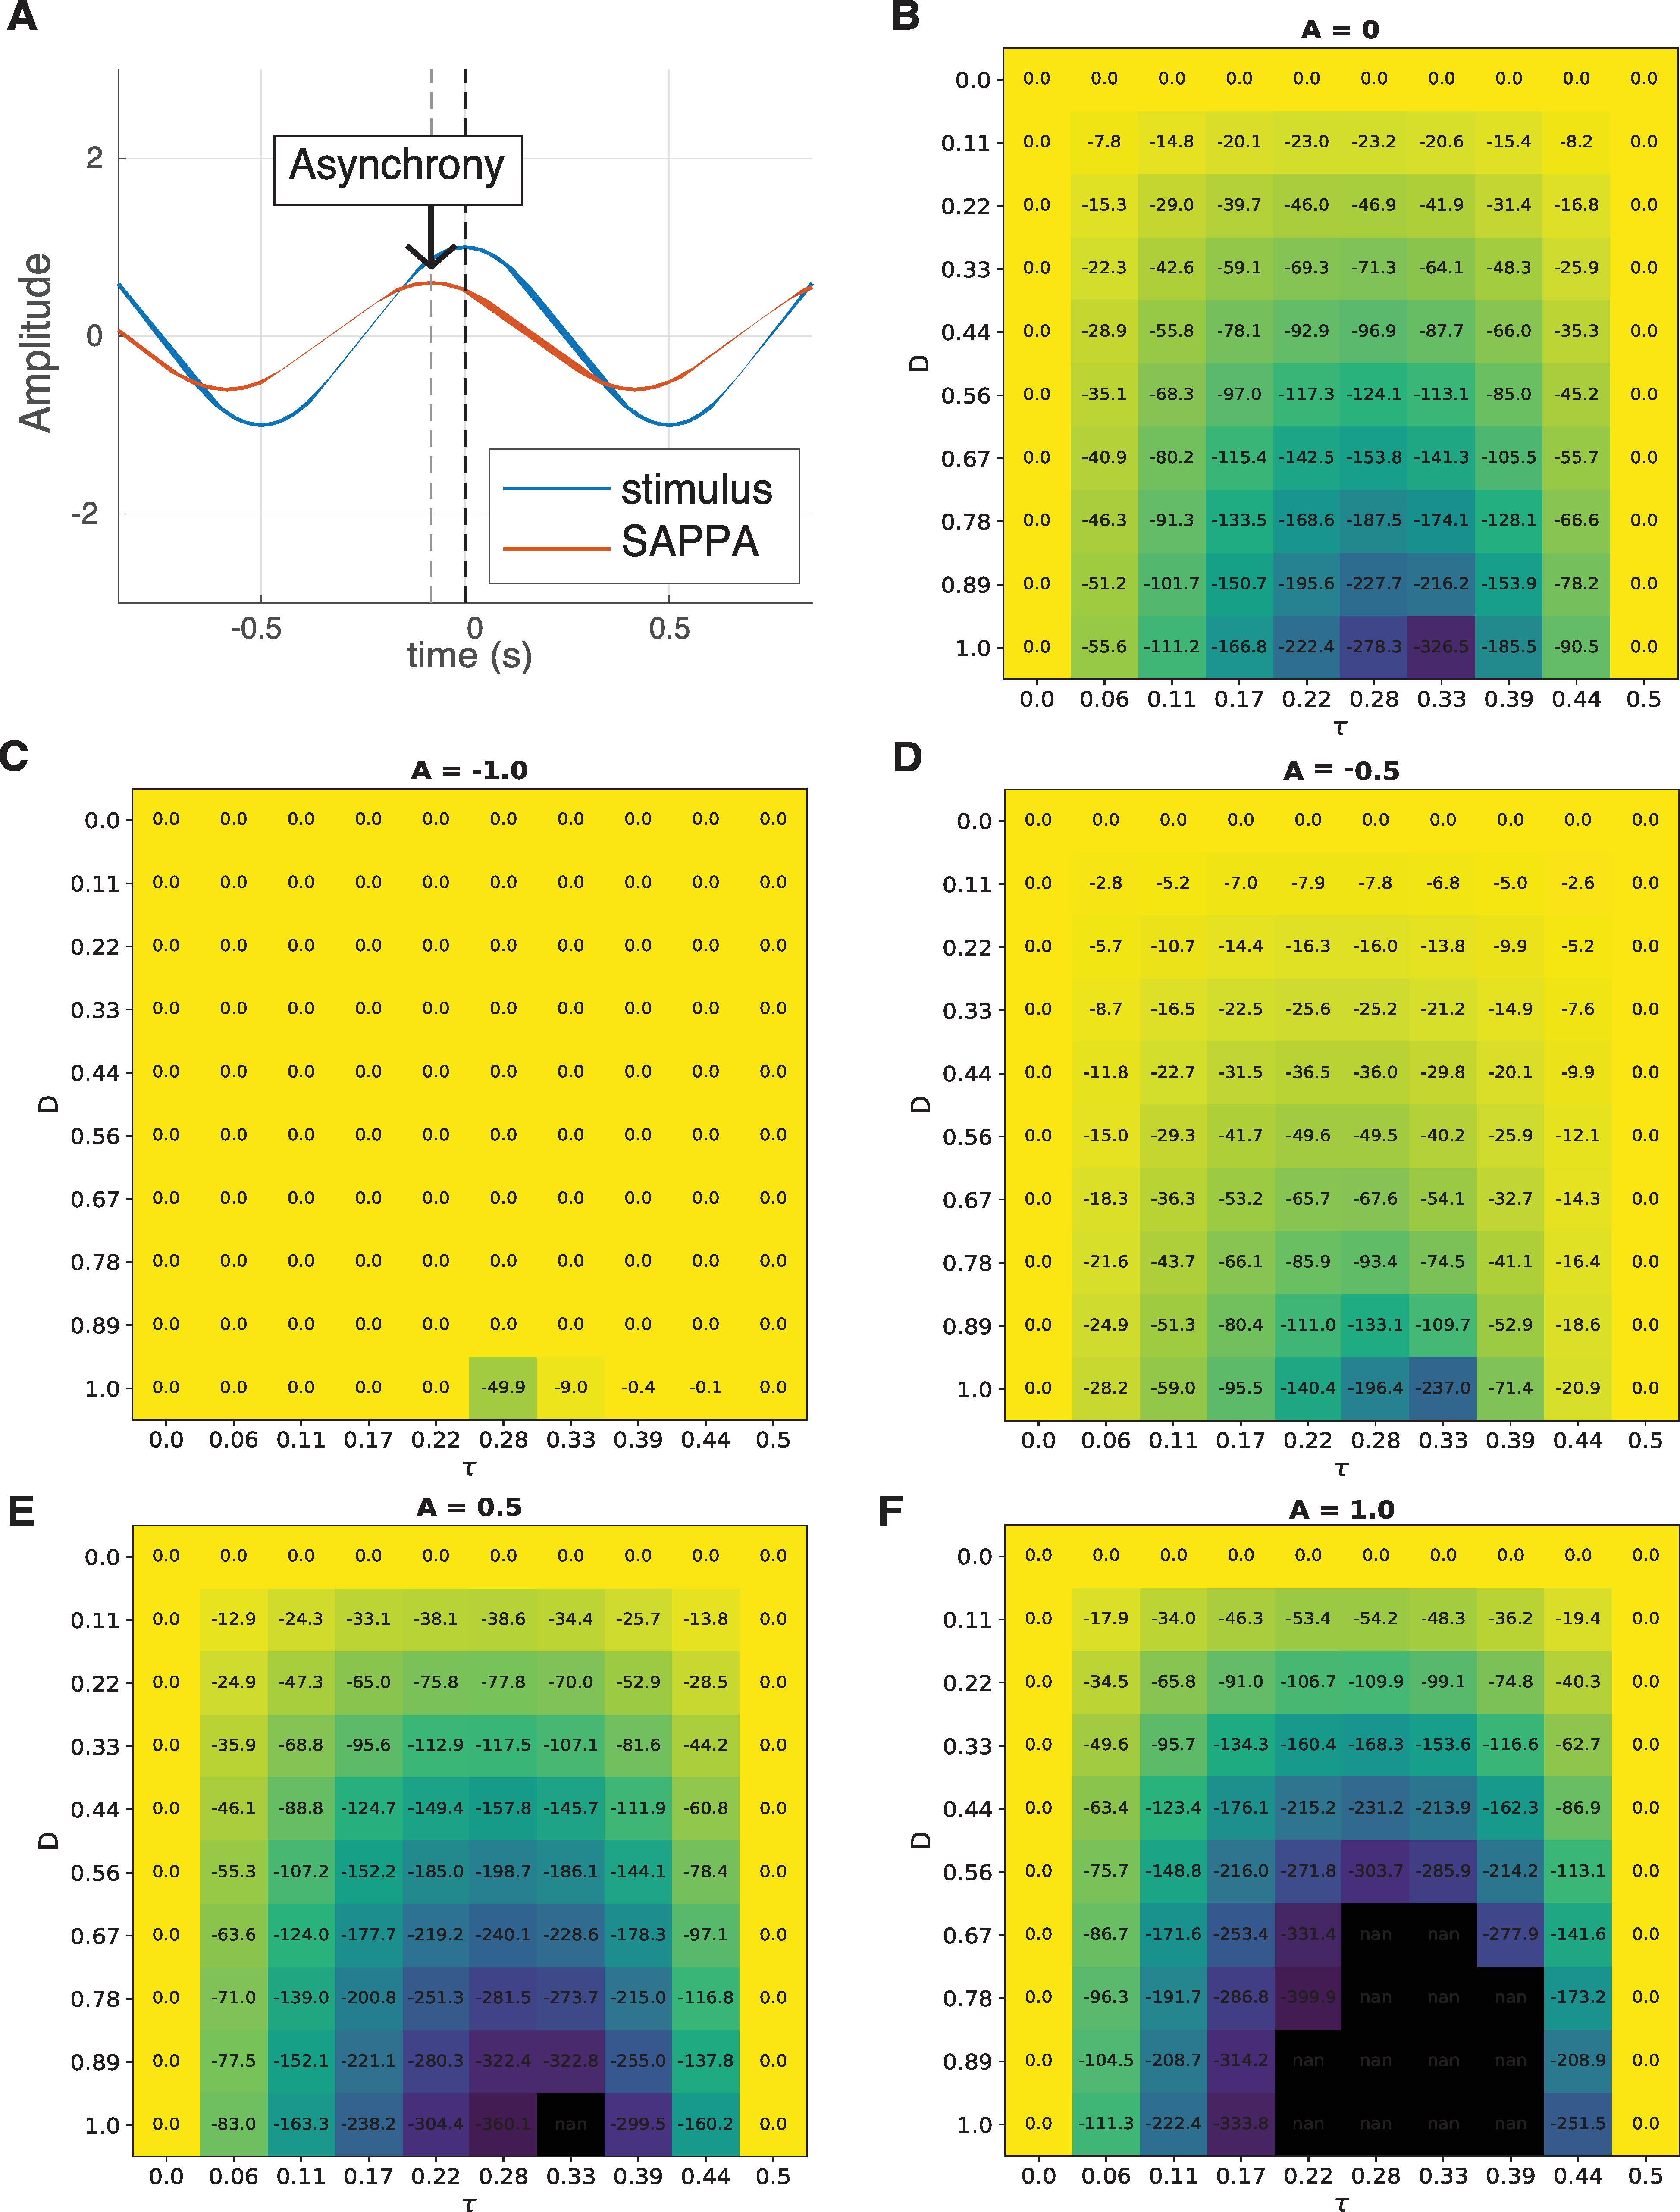
\includegraphics[width=0.8\textwidth]{figures/fig2_6.png}
    \caption[Analysis of the effect that different parameters in the SAPPA model have on its anticipation tendency]{\textbf{Analysis of the effect that different parameters in the SAPPA model have on its anticipation tendency.} (A) Illustration of what the asynchrony between the SAPPA model and the external sinusoidal stimulus can look like, and how it's measured. (B-F) Analysis of the anticipation as a function of $D$ and $\tau$ in Eq \eqref{eq:2.5}, and $A$ in Eq \eqref{eq:2.7}: (B) $A = 0$, (C) $A = -1.0$, (D) $A = -0.5$, (E) $A = 0.5$, (F) $A = 1$. In these analyses (B-F) the parameter $f = 1$. The numbers in each cell indicate the anticipation (in ms) observed when the SAPPA model synchronized with the external sinusoidal stimulus. A black cell indicates that the SAPPA model did not synchronize with the external sinusoidal stimulus and hence the asynchronies could not be computed. In the analyses (B-F), the asynchrony quickly moves away from zero as $0 < \tau < 0.5$, especially when $D = 1$. Additionally, we explored how different initial conditions affect the model's asynchrony and discontinuities, described in the Supplementary Fig.{} \ref{fS_2} which contains the bifurcation diagram for the SAPPA model when $D = 1$.} 
    \label{f2_6}
\end{figure}

For this parameter analysis we fixed $f = 1$ to ignore its scaling effect. We analyzed the effect of $D$ in the range of values between $0$ and $1$, which is the dynamic range of $z$ when $F = 0$ and $D = 0$, and also the dynamic range of $F$, considering all three Eqs \eqref{eq:2.6}, \eqref{eq:2.7} or \eqref{eq:2.8}. For $\tau$, we analyzed its effect in the range of values from $0$ seconds to $0.5$ seconds, because the period associated with $f = 1$ is one second and a processing delay with duration closer to the stimulus period length would not make sense during synchronization. To observe the effect of $A$, we also tested $A = -1$, $-0.5$, $0$, $0.5$, and $1$, which are all values within the dynamic range of $z$ (when $F = 0$ and $D = 0$) and $F$ (note that when $A = 0$, Eqs \eqref{eq:2.6} and \eqref{eq:2.7} are the same).

We evaluated the anticipation for all possible combinations of $D$, $\tau$, and $A$ parameters. At the beginning of each simulation, the phase of $z$ was initialized to zero. During the first few sinusoidal cycles, the SAPPA model phase-locked with the external sinusoid in order to achieve a state of stable synchronization. From a dynamical systems perspective, `synchronization' refers to the relationship between one system's actions as closely adhering to another system's actions \cite{pecora1990synchronization}. Stable synchronization was observed when the phase difference between the stimulus sinusoid and the model's oscillators reached a constant value over time. This stable mode is known in dynamical systems theory as a steady state. Fig.{} \ref{f2_6}D shows how we calculated the asynchrony between our model's oscillator $z$ and the stimulus sinusoid. After a simulation reached a steady state, we first found the timepoints of the peaks for the real part of the $z$ oscillator and the stimulus sinusoid. Then, we subtracted each stimulus sinusoid's peak time from the nearest $z$ oscillator's peak time. The average peak time difference between the stimulus sinusoid and the $z$ oscillator over time was considered the model's mean asynchrony. Our results are shown in Fig.{} \ref{f2_6}. To visualize the results of these simulations, we plotted these results in matrix form, with the x axis indicating the value of $\tau$, the y axis the value of $D$, and the color in the matrix cells indicating the asynchrony. We obtained five matrices, one for each of the five values of $A$ tested.

\subsection{Experiment 1: Individual tapping in synchronization with an \\ isochronous stimulus}

\subsubsection{Behavioral data for simulation}

In the task by Repp and Doggett \cite{repp2007tapping}, musicians and non-musicians tapped in synchrony with an isochronous metronome in a frequency range between 1Hz and 0.29Hz (corresponding to period durations between 1000ms and 3500ms). They found that the anticipatory tendency increased as a function of metronome period length. Fig.{} \ref{f2_2}B shows our models' anticipation, as well as the linear regression on the behavioral data (Fig.{} 1A in Repp and Doggett \cite{repp2007tapping}). We computed the linear regression lines as the best fit on the anticipation values for musicians and non-musicians.

\subsubsection{Setup, procedures and measurements}

Fig.{} \ref{f2_1}A shows the human task and a graphical explanation of our simulation setup that contain the SAPPA model and the input stimulus. In these simulations, the input $F$ was $F = \exp(i2\pi f_s t) + Az$ because our model ``listened" to itself (i.e., received its own instantaneous activity as input). In the parameter analysis section above, we studied the model's behavior for a frequency of 1Hz. In the human task simulated in this experiment, humans tapped with metronomes of period lengths between 3500ms (approx. 0.2857Hz) and 1000ms (1Hz). Hence, we repeated the parameter analysis with $f = 0.285$ (Fig.{} \ref{f2_7}) to observe the model's behavior at the other end of the spectrum of stimulus frequencies corresponding to this human task. Remember that $f = f_s$. always, unless otherwise noted.

\begin{figure}
    \centering
    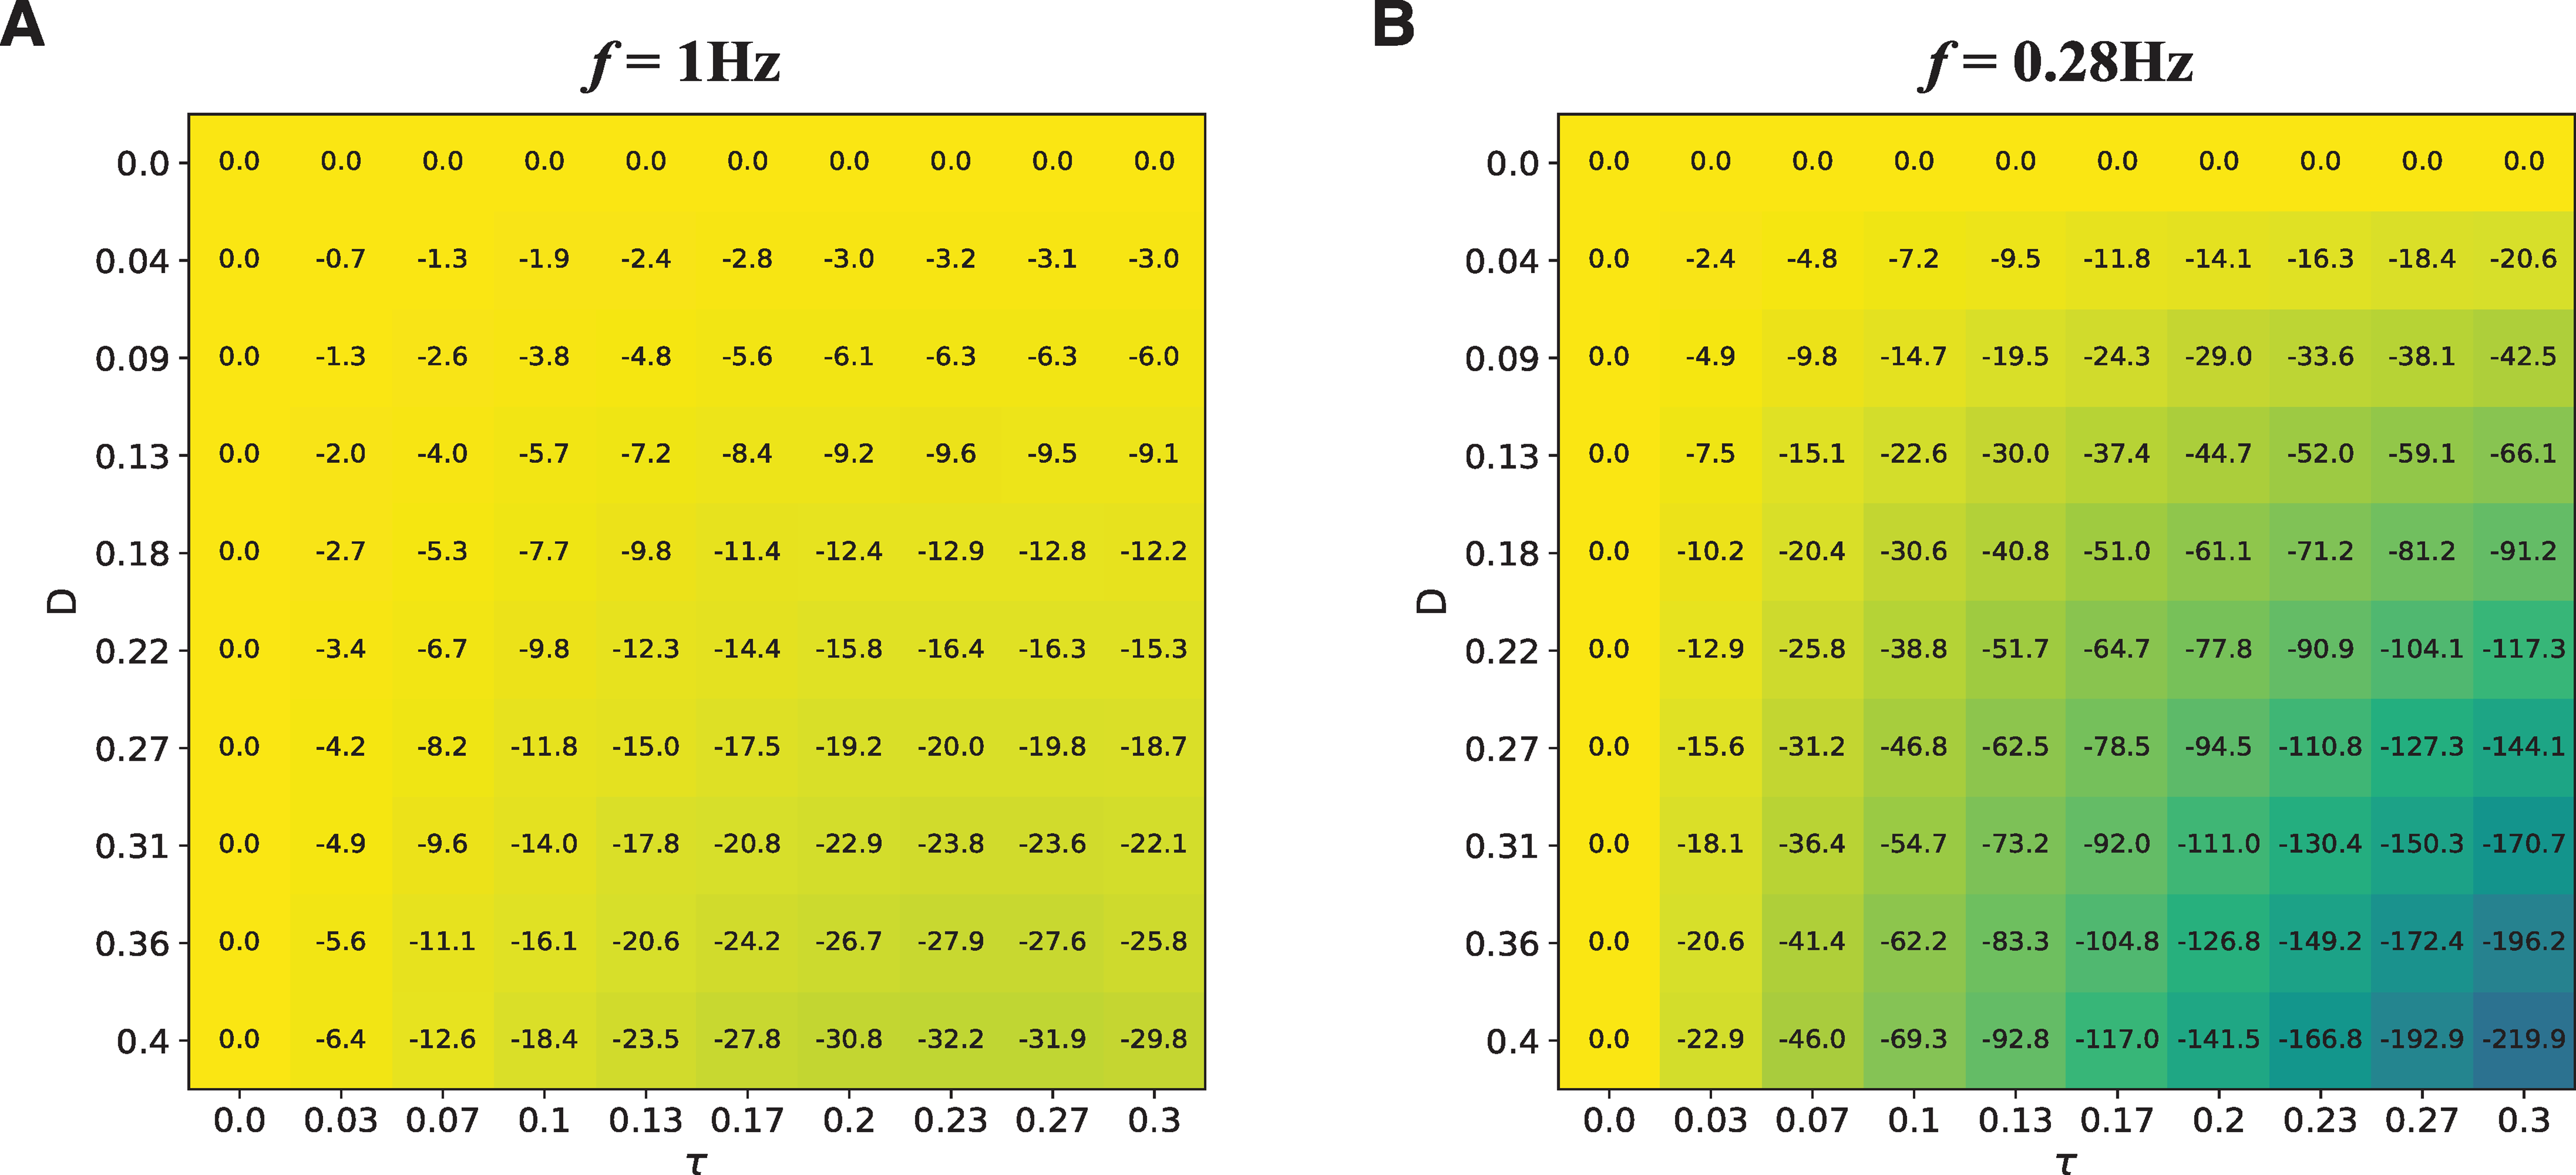
\includegraphics[width=1.0\textwidth]{figures/fig2_7.png}
    \caption[Analysis of the effect that different frequencies in the SAPPA model have on its anticipation]{\textbf{Analysis of the effect that different frequencies in the SAPPA model have on its anticipation.} (A) Analysis of the anticipation as a function of $D$ and $\tau$ in Eq \eqref{eq:2.5} when $A = -0.5$ and $f = 1$. (B) Analysis of the anticipation as a function of $D$ and $\tau$ in Eq \eqref{eq:2.5} when $A = -0.5$ and $f = 0.2857$. The numbers in the cells indicate the anticipation (in ms) observed when the SAPPA model synchronized with the external sinusoidal stimulus.}
    \label{f2_7}
\end{figure}

\subsubsection{Model optimization}

To identify the model matching the musician and the non-musician anticipation curves, we identified the set of parameters $D$, $\tau$, and $A$ that resulted in the best fit between the simulated model's anticipation and the slopes of the linear regression for the behavioral data (Fig.{} \ref{f2_2}B). We found that $A = -0.5$, $\tau = 0.222$ seconds, and $D = 0.05$ for the musician SAPPA model and $D = 0.36$ for the non-musician SAPPA model.

For all experiments that we conducted $A = -0.5$. This implies that our model's behavior is half of the magnitude of the external stimulus $\exp(i2\pi f_s t)$, which always has a magnitude of $1$, meaning that the model is forced more strongly by the external sinusoidal stimulus than by its own activity and that the SAPPA model's phase-locking behavior will be greatly determined by the phase of the external sinusoid \cite{kim2015signal}. In the SAPPA model, all recurrent feedback terms are negative. That is why $A = -0.5$ is negative in Eqs \eqref{eq:2.7} and \eqref{eq:2.8}, like the delayed recurrent feedback term in Eq \eqref{eq:2.5}. In Eq \eqref{eq:2.7}, $z$ affects the encoding of the external stimulus, shifting the phase of $F$ in a negative direction with respect to $\exp(i2\pi f_s t)$. Behaviorally, this means that when the SAPPA model listens to itself in addition to the stimulus $\exp(i2\pi f_s t)$, its actions will be more aligned with $F=\frac{\exp(i2\pi f_s t)+Az}{|\exp(i2\pi f_s t)+Az|}$, thus resulting in reduced anticipation compared to when $F = \exp(i2\pi f_s t)$.

\subsection{Experiment 2: Interpersonal synchronization during alternating \\ paced tapping with or without auditory feedback}

\subsubsection{Behavioral data for simulation}

Among the behavioral data shown by Nowicki and colleagues \cite{nowicki2013mutual}, we were focused on simulating the results from solo and duet tasks. First, in the solo task, musicians tapped every other beat in synchrony with a metronome while hearing their own taps (feedback-on) or only hearing the metronome (feedback-off). This means that musicians' tapping behavior had a subharmonic rate with the stimulus rate (i.e., if the stimulus was presented at 2 Hz, tapping should occur at 1 Hz). As shown in Fig.{} \ref{f2_3}A, anticipation was larger when musicians could not hear their own taps compared to when they did. Second, in the duet task, pairs of musicians alternately tapped with a metronome while hearing their own and the partner's taps (feedback-on) and also while only hearing the metronome (feedback-off). The anticipation was also larger when musicians could not hear each other in the duet task, as shown in Fig.{} \ref{f2_3}D.

\subsubsection{Setup, procedures and measurements}

To simulate the feedback-off condition, we removed the $z$ term in the $F$ input, meaning that the model received input only from the external sinusoid $F = \exp(i2\pi f_s t)$. To simulate the feedback-on condition, we added the model's own $z$ activity to the input $F$ during the second half of every stimulus cycle. Finally, to simulate the duet task, we connected two SAPPA models, both synchronizing with the same external sinusoid. One of the SAPPA models exhibited in-phase synchronization with the external sinusoidal stimulus and the other one synchronized antiphase with respect to the external sinusoidal stimulus. To achieve in-phase and antiphase synchronization, the sinusoidal stimulus had a positive sign (i.e., $F = \exp(i2\pi f_s t)$) and a negative sign (i.e., $F = -\exp(i2\pi f_s t)$), respectively. To simulate the feedback-on condition, the two synchronizing SAPPA models alternately received one of the model's $z$ activity as input during the first half of every stimulus cycle, and the other model's $z$ activity during the second half of every stimulus cycle.

We used the SAPPA model and the parameter set determined for musicians' data in Experiment 1. The simulations of the solo task started with a musician SAPPA model receiving an external sinusoid of frequency $f_s = 1$Hz (similarly, the SAPPA model's $f = 1$Hz). To simulate the solo task with auditory feedback, we observed the model's behavior while its own $z$ activity was added as an additional input during the second half of every stimulus cycle (feedback-on) (see Fig.{} \ref{f2_1}B). This means that, the input alternates between $F = \exp(i2\pi f_s t)$ and $F = \exp(i2\pi f_s t) + Az$ at a frequency twice as fast as the external sinusoid, to follow the task design (e.g., listening to a metronome click, then listening to both a metronome click and own tapping). To simulate the condition without auditory feedback, the external sinusoid was set as the only input throughout the simulation (feedback-off, the input was always $F = \exp(i2\pi f_s t)$). This task design and the corresponding model setup are indicated in Fig.{} \ref{f2_1}B and \ref{f2_1}C, respectively.

To simulate the duet task indicated in Fig.{} \ref{f2_1}D, we paired two models, of which one was referred to as model 1 and the other as model 2. To simulate the duet condition with auditory feedback, the input to model 1 was set to $F = \exp(i2\pi f_s t) \pm Az(k)$, while the input to model 2 was set to $F = -\exp(i2\pi f_s t) \pm Az(k)$, where $|A| = 0.5$ and $k$ alternated between 1 and 2 at a rate twice as fast as the frequency of the external sinusoid, as illustrated in Fig.{} \ref{f2_1}D. As stated earlier, the sign of $\pm Az(k)$ depends on whether $z$ indicates recurrent feedback (positive) or the other model's activity (negative). To simulate the duet condition without auditory feedback, both models received only the external sinusoid as input ($F$ was always $F = \exp(i2\pi f_s t)$ for model 1 and $F = -\exp(i2\pi f_s t)$ for model 2). Fig.{} \ref{f2_1}E illustrates the simulation of the condition without auditory feedback.

The mean asynchrony between the stimulus and the in-phase synchronizing model was computed in the same manner as Experiment 1, as the difference between the peak of the real part of the models' oscillation and the closest peak timepoints in the real part of the stimulus sinusoid. The mean asynchrony between the stimulus and the anti-phase synchronizing model was computed as the difference between the peak of the real part of the models' oscillation and the closest valley timepoints in the real part of the stimulus sinusoid.

\subsubsection{Model optimization}

The SAPPA models in this experiment were the same musician and non-musician models identified in Experiment 1. Therefore, the model architecture used in this experiment is summarized by Eq \eqref{eq:2.5}. Simulations lasted a total of 20 seconds.

\subsection{Experiment 3: Interpersonal synchronization during rhythm-\\ clapping alternation in the presence of transmission latencies}

\subsubsection{Behavioral data for simulation}

In the behavioral paradigm used by Chafe and colleagues \cite{chafe2010effect}, two musicians in different rooms alternately clapped a staggered and looping rhythmic pattern together for an extended period of time. TLs were introduced between the musicians to simulate transmission delays over the internet when remotely located individuals play music together. Such latencies via an internet connection typically range from 20ms to 100ms \cite{caceres2010jacktrip, caceres2008edge}. The rhythmic task consisted of three claps interspaced with periods of relative length of 1-1-2. The two musicians synchronized and performed the pattern in a staggered manner with a half pattern overlap; the first musician started the first half of the pattern with doing two claps (1-1-) alone, and at the third clap (2-), the starting point of the second half of the pattern, the second musician started the first half of the pattern from the beginning (1-1-). When the second musician started the second half of the pattern (2-), the first musician returned to the first half of the pattern (1-1-) and so on. They repeated this without interruption for about 30 s (see Fig.{} \ref{f2_1}F). Before starting, the first musician heard a metronome for six counts. The metronome was randomly set at a tempo of either 86 bpm (beat-per-minute), 90 bpm, or 94 bpm to avoid habituation effects. The second musician did not hear the metronome and joined after hearing the auditory outcomes of the starter's actions for the first half of the pattern. Delivery of auditory outcome information between subjects was bidirectionally delayed by a TL. For a given trial, the latency stayed at a constant value. Latencies between 3ms and 78ms were examined. The results show that with TLs longer than 20ms the two musicians decelerated their common tempo. For the latencies shorter than 10ms, they accelerated instead. As shown in Fig.{} \ref{f2_4}B, the asynchrony between the two musicians at every cycle grew as a function of the TL.

\subsubsection{Setup, procedures and measurements}

To simulate this paradigm, we used a pair of musician SAPPA models like the one developed in Experiment 1, and set them up to feed one model's $z$ activity as an input to the other at a given cycle, then alternate this input flow direction (see Fig.{} \ref{f2_1}F). The first model is considered to be the initiator and the other, the joiner. In our simulations, $f$ for both oscillators was set to be a frequency of 1.5Hz, equivalent to 90 bpm. For the sake of simplicity, we did not employ the nearby offsets of this frequency that were used by Chafe and colleagues \cite{chafe2010effect} to mitigate adaptation to a specific tempo by the subjects. The simulations were also carried out with pairs of non-musician SAPPA models. Compared to Experiment 1 and Experiment 2 where an external sinusoid stimulated the SAPPA model, in Experiment 3 pairs of oscillators stimulated each other, and there was no external sinusoid.

A simulation of the original experiment began by allowing the initiator SAPPA model to oscillate for one cycle. During this cycle, the initiator received its own $z$ activity as an input (the input to the initiator was $F = Az(1)$) and sent its $z$ activity as an input to the joiner (the input to the joiner was $F = z(1)$). After receiving an input from the initiator for one cycle, the joining model continued oscillating one cycle getting its own $z$ activity as an input (the input to the joiner was $F = -Az(2)$) and sending its $z$ activity to the initiator (the input to the initiator is then $F = z(2)$). In subsequent cycles, the inputs to the two models continued alternating every cycle which oscillator's $z$ activity was used as the inputs to both oscillators. At a given cycle, whichever model's $z$ activity was used as an input to both models was referred to as the `active' model, while the other one was referred to as the `passive' model. This alternation was repeated until the simulation had run for 30 seconds to complete a trial. Trials were carried out in the presence of fixed TLs ranging from 0ms to 78ms between models.

We measured the Lead/Lag relationship between models in the same way as Chafe and colleagues \cite{chafe2010effect}. For each participant clapping in turn, the Lead/Lag relationship with respect to the other participant was measured as: 

\begin{equation}
L = (a(1) - b(1)) + (b(2) - a(2)) \label{eq:2.9}
\end{equation}

Where $a(1)- b(1)$ is the time difference in seconds between the first clap of the participant currently in turn and the last clap of the participant previously in turn. $b(2)–a(2)$ is the time difference between the first clap of the participant clapping after the current participant in turn and the last clap of the current participant in turn. $L$ can be expressed as a fraction of a 90 bpm tempo, as in Chafe and colleagues \cite{chafe2010effect}, using the expression: $- 90 \times L \div (60 \times 1000)$, where $L$ (in ms) gets converted to a fraction of a period corresponding to a 90bpm tempo. If the resulting value was negative, this meant that the passive oscillator lagged behind the active oscillator. A positive value suggests the opposite.

\subsubsection{Model optimization}

The SAPPA model in this experiment was similar to the musician and non-musician models identified in Experiment 1. Therefore, the model architecture used in this experiment is summarized by Eq \eqref{eq:2.5}. Compared to Experiments 1 and 2, in this experiment these was no external sinusoidal stimulus. Instead, pairs of SAPPA models stimulated each other.

\chapter{Hebbian learning with elasticity explains how a musician's spontaneous motor tempo affects periodic synchronization}
\chaptermark{Hebbian learning explains musician synchronization}

\section{Abstract}
Music has a tempo (or frequency of the underlying beat) that musicians maintain throughout a performance. Musicians maintain this musical tempo on their own or paced by a metronome. Behavioral studies have found that each musician shows a spontaneous rate of movement, called spontaneous motor tempo (SMT), which can be measured when a musician spontaneously plays a simple melody. Data shows that a musician's SMT systematically influences how actions align with the musical tempo. In this study we present a model that captures this phenomenon. To develop our model, we review the results from three musical performance settings that have been previously published: (1) solo musical performance with a pacing metronome tempo that is different from the SMT, (2) solo musical performance without a metronome at a spontaneous tempo that is faster or slower than the SMT, and (3) duet musical performance between musician pairs with matching and mismatching SMTs. In the first setting, the asynchrony between the pacing metronome and the musician's tempo grew as a function of the difference between the musician's SMT and the metronome tempo. In the second setting, musicians drifted away from the initial spontaneous tempo toward the SMT. And in the third setting, the absolute asynchronies between performing musicians were smaller if their SMTs matched compared to when they did not. Based on these previous observations, we hypothesize that, while musicians can perform musical actions at a tempo different from their SMT, the SMT constantly acts as a pulling force. We developed a model to test our hypothesis. The model is an oscillatory dynamical system with Hebbian and elastic tempo learning that simulates music performance. We simulate an individual's SMT with the dynamical system's natural frequency. Hebbian learning lets the system's tempo adapt to match the stimulus tempo. The SMT's pulling force is simulated with an elasticity term that pulls the instantaneous tempo toward the system's natural frequency. We used this model to simulate the three music performance settings, replicating behavioral results. Our model also lets us make predictions of musician's performance not yet tested. The present study offers a dynamical explanation of how an individual's SMT affects adaptive synchronization in realistic musical performance.

\section{Introduction}
Humans can seamlessly sing a song in the shower or walk on an empty street. In such a solo setting, individuals show a spontaneous singing tempo or walking pace. In everyday life, however, humans often have to synchronize with external signals. For example, singing with a pre-recorded song or marching in a parade with other individuals. In the specific case of musical performances, musicians change the tempo of their actions to match a musical tempo that is kept by the group of performing musicians. When musicians synchronize with each other they carry out perception-action coordination (PAC), which involves the coordinated communication between the brain's sensory areas that perceive stimuli and the motor system that executes actions \cite{ridderinkhof2014neurocognitive}. However, most musical performances do not match a musician's spontaneous tempo. How a musician's spontaneous tempo affects a musical performance is still an open question \cite{zamm2018musicians}. To tackle this question, one must first study an individual's spontaneous tempo of periodic action, like finger tapping. The spontaneous motor tempo (SMT) can be obtained by calculating the average inter-onset interval (IOI) between consecutive periodic actions \cite{mcauley2006time}. In music, where the rhythm is most often periodic but consecutive events may not share an IOI, we measure the inter-beat interval (IBI). 

Before diving deep into our overview of previous research, we must clarify some important terminology. In general, to measure periodic phenomena one can use the term frequency in units of hertz (cycles or events per second). However, to measure the period of time between isochronous events (like a metronome) we can use the IOI in units of (milli)seconds. In music, not all events are isochronous. Nonetheless, most music has a periodic tempo (or frequency of the underlying beat) which is measured in units of beats per minute (BPM) in the fields of music theory, musicology, and music performance. The period of time between beats in music can be measured with the IBI in units of (milli)seconds. The IOI and IBI share the same units of (milli)seconds because they measure the period of time between isochronous events or musical beats, respectively. One should not confuse the units of musical tempo and the SMT due to the fact that both have the word `tempo' in their name. In fact, the SMT having units of (milli)seconds is incorrect, by definition. The word `tempo' implies a frequency, so proper units for such a mesurement could be hertz (Hz) or BPM. A correct name for the SMT would be the `spontaneous motor period' (SMP) because it is measured in units of (milli)seconds, and the SMT should be measured in BPM like the musical tempo. Similar to the SMT, the term `spontaneous performance rate' (SPR), measured in (milli)seconds, has been used to describe the musical tempo shown by individuals when asked to spontaneously play a simple melody \cite{zamm2016endogenous}. The term SPR is also incorrect, just like the SMT, and it should have been called the `spontaneous performance period' (SPP) because it is measured in units of (milli)seconds. Here we have acknowledge these unfortunate misnomers because we will use the correct terminology when describing our experiments. However, when describing previous studies, we will still use the SMT term in the original context, clarifying if its use is incorrect. 

SMTs vary within individuals, tending to be faster in early childhood compared to adulthood \cite{mcauley2006time}, and between individuals, tending to be slower in adult musicians (SMP of $\sim$ 400ms IOI on average) compared to non-musicians (SMP of $\sim$ 300ms IOI on average) \cite{scheurich2016spontaneous, drake2000tapping}. After studying the SMT, one can study how individuals synchronize a simple movement, like finger-tapping, with a metronome. The asynchrony between the individual's taps and metronome clicks can be measured, and the mean asynchrony (MA) can be calculated \cite{repp2005sensorimotor, repp2013sensorimotor}. For both musicians and non-musicians the MA tends to be negative (taps precede the metronome click) when synchronizing with a metronome with an IOI between 300ms and 2000ms \cite{mates1994temporal}. However, the MA becomes smaller as the metronome IOI approaches 300ms and for an IOI smaller than 300ms the MA is absent or even slightly positive \cite{repp2003rate, wohlschlager1999synchronization}. Interestingly, the 300ms IOI, around where the negative MA disappears, coincides with the mean SMP observed in humans ($\sim$ 350ms), indicating a possible connection between SMP and MA dynamics. Additionally, the MA is also positive (taps lag the metronome clicks) when synchronizing with a very slow metronome with IOIs greater than 5000ms \cite{miyake2004two}. Synchronization with a slow metronome is a difficult task, so the positive MA in this case is the result of musician actions reacting to the metronome clicks, rather than a direct relationship between the MA and the SMP \cite{repp2007tapping}. When synchronizing with a metronome with an IOI between 2000ms and 5000ms, the human actions form a bimodal distribution (i.e., some taps precede and some lag the metronome clicks) \cite{baaaath2016estimating}. However, musical expertise does affect the MA, with musicians showing overall smaller MAs compared to non-musicians \cite{repp2007tapping}. Together, the SMT/SMP and the MA are behavioral correlates of PAC. While the SMT/SMP is a measurement of spontaneous, non-paced action, the MA is a measurement of paced action. Studying both the SMT/SMP and the MA lets us better understand how the spontaneous tempo of periodic action affects an individual's synchronization with an external periodic stimulus.

Previous studies have looked at musical performance in solo and group settings to investigate how the SMT/SMP and the MA are related to each other. In one study, musicians performed a melody in a solo setting synchronizing with a metronome tempo that was faster or slower than the musician's SMT. Results showed that the MA grew as a function of the absolute difference between the musician SMT and the metronome tempo. Additionally, when the metronome was faster than the SMT, the MA had a tendency to be positive (taps lagged the metronome clicks), and when the metronome was slower than the SMT, the MA had a tendency to be negative (taps preceded the metronome clicks). The smallest MA was observed when the metronome tempo matched the individual's SMT \cite{scheurich2018tapping}. In another study, musician performed a melody in a solo setting without a metronome, starting at spontaneous tempo that was slower or faster than the SMT. Results showed that the musician's tempo had a tendency to drift back to the SMT \cite{zamm2018musicians}. This tendency to drift back to the SMT has also been observed in other similar studies \cite{mcauley2006time, yu2003task}. One study has also investigated the relationship between the SMT and the MA in duet musical performances. Musicians were split into two groups: one group consisted of musician pairs with matching SMT (SMP difference smaller than 10ms) and the other group consisted of musician pairs with mismatching SMT (SMP difference greater than 110ms). Next, pairs of musicians were asked to perform a melody with each other. Musician duets with matching SMTs showed a smaller mean absolute asynchrony compared to synchronizing pairs with mismatching SMTs. Additionally, after the duet performance each musician's SMT/SMP was remeasured, and results showed that each musician's SMT/SMP did not change compared to the SMT/SMP measured before the duet performance \cite{zamm2016endogenous}. This study analyzing musical performance in a duet setting revealed that the SMT/SMP affects the MA in social tasks requiring periodic synchronization (i.e., rowing or playing music), but the task did not affect each musician's SMT/SMP \cite{zamm2016endogenous}. The evidence from all these studies in both solo and duet settings highlights the effect that the SMT/SMP has on both the MA and the musical tempo.

Theoretical models have previously described the mechanisms that give rise to the SMT/SMP and the MA, but independently. Potential mechanisms of the SMT/SMP include motor resonance governed by body weight and limb length \cite{goodman2000advantages} and central pattern generators in the brain that are essential for motor control \cite{latash1992virtual, wolpert2007probabilistic}. Mechanisms that give rise to the MA include delayed recurrent feedback in central-peripheral communication between the auditory and motor systems \cite{stepp2010strong, roman2019delayed, aschersleben2002temporal} and under- or over-estimation of IOI lengths \cite{loehr2009subdividing}. Currently, a complete explanation of how the SMT/SMP and the MA relate to each other is missing, but the synchronization dynamics of non-linear oscillators can capture some of these relationships. Non-linear oscillator models capture an individual's SMT using an oscillator's natural frequency \cite{large2002tracking, large2002perceiving, mcauley2006time}. Additionally, non-linear oscillators can synchronize in-phase with a periodic stimulus with a frequency that is different but close to the natural frequency. In such a scenario, a MA is observed between the oscillator and the stimulus. Similar to observations made in humans \cite{scheurich2018tapping}, the MA shrinks as the difference between the natural frequency and the stimulus frequency is reduced \cite{kim2015signal, kim2019mode}. As a result, a non-linear oscillator can capture how a musician's MA grows as a function of the difference between musician's SMT and stimulus tempo. Moreover, after a non-linear oscillator is phase-locked to the stimulus frequency, if the stimulus disappears the oscillator will continue oscillating but will spontaneously return to its natural frequency \cite{kim2015signal, kim2019mode}, just like musicians show a tendency to return to their SMT in the absence of a pacing stimulus \cite{zamm2018musicians} or after a musical performance \cite{zamm2016endogenous}. However, these observations in non-linear oscillators require the natural frequency and the stimulus frequency to be relatively close to each other, and if the difference exceeds a certain threshold, in-phase synchronization will not be possible and unsynchronized behavior may be observed \cite{kim2015signal, kim2019mode}. This is different than the synchronization abilities of humans, who can synchronize with stimuli tempi that are relatively far away from their SMT. Hence, a model consisting purely of non-linear oscillators has a limited potential to fully capture the relationship between the SMT and the MA in humans.

Righetti and colleagues described oscillators equipped with a frequency learning rule allowing them to adaptively change their frequency to match the frequency of an external periodic stimulus, regardless of the oscillator's natural frequency \cite{righetti2009adaptive}. A limitation of the model by Rigetti and colleagues is that, unlike humans, the oscillators with frequency learning capabilities do not return to their natural frequency after stimulation ceases. An individual's SMT is recovered after synchronizing with a periodic stimulus with an arbitrary tempo \cite{scheurich2018tapping}. This phenomenon could be explained by the SMT having an elastic force. This hypothesis proposes that the SMT is an attractor state pulling the system's tempo towards optimal energy usage \cite{mcauley2006time, scheurich2018tapping}, like a flexible piece of rubber that returns to its original state when no external energy is applied to it \cite{strogatz1993coupled}. Lambert and colleagues added a linear elasticity force governed by Hooke's law to the frequency learning rule described by Righetti and colleagues \cite{lambert2016adaptive}. This elasticity term pulls the oscillator's frequency to its natural frequency. Hence, the oscillator can match its frequency with an external stimulus frequency, but a force is constantly pulling the oscillator's frequency to its natural frequency. If the stimulus ceases, the oscillators frequency will return to the natural frequency.

Behavioral studies had proposed an elastic and adaptive tempo learning hypothesis to explain the relationships between the SMT/SMP and the MA in humans \cite{scheurich2018tapping}. However, no study so far has quantified how well a dynamical systems model with elastic frequency learning could capture dynamics observed in human data. In this study we test this hypothesis using an oscillatory dynamical systems model equipped with Hebbian learning for frequency adaptation and an elastic force constantly pulling to the natural frequency. More specifically, we use the oscillators described by Large and colleagues \cite{large2010canonical} and we equip them with elastic frequency learning \cite{righetti2009adaptive, lambert2016adaptive}. The goal is to validate the model using real human data from previous studies of musical performance that analyzed the relationships between the SMT/AMP and the MA. If we can achieve our goal, we will mechanistically show how an individual's SMT/SMP affects the MA during PAC with a stimulus that is either a metronome or another synchronizing individual. Our modeling approach is appropriate because oscillators have a fixed natural frequency observed spontaneously in the absence of an external stimulus. This natural frequency simulates an individual's SMT. Because our model has an elastic frequency learning rule, it can adapt its frequency to synchronize with a periodic stimulus of any frequency, but always showing an MA due to the elastic force constantly pulling the oscillator's frequency to its natural frequency. This elastic frequency learning rule simulates two human features. First, the ability to synchronize with a broad range of periodic stimulus tempi. And second, the constant SMT displayed by humans, even after synchronizing with a stimulus of a different tempo. 

Given all of its features, we refer to our model as the Adaptive Synchronization with Hebbian Learning and Elasticity (ASHLE). The ASHLE model is inspired by neuroscientific hypotheses about the mechanisms of PAC. The methods section gives the complete definition of ASHLE, but here we briefly describe its main properties. ASHLE consists of two oscillators. The first one is stimulated by an external stimulus, and simulates perception and auditory-motor neural entrainment with the stimulus frequency \cite{large2015neural, patel2014evolutionary, daly2014changes, grahn2009feeling, grahn2013finding}. This first oscillator is equipped with the Hebbian frequency learning rule to learn the frequency of the external stimulus. The second oscillator receives the activity of the first oscillator as input, and simulates the motor system planning that controls peripheral effectors and their actions (i.e., a finger playing a piano). This second oscillator is equipped with elastic Hebbian frequency learning to learn the stimulus frequency, filtered by the first oscillator, while constantly being pulled to its natural frequency. The timescale of the Hebbian frequency learning is relatively fast (see the parameter analysis in the methods section). In contrast, the first oscillator additionally receives a small input from the second oscillator, forcing the first oscillator to return to the natural frequency, at a very slow timescale, in the absence of a stimulus. 

ASHLE only simulates the musical beat in a musical performance and not any other spectral features like pitch, harmony or melody content. However, because our goal is to simulate the dynamics of the MA and the SMT/SMP at the level of musical beat performance, ASHLE is an adequate model. Below we describe three experiments (see Fig.{} \ref{f3_1}) we carried out with ASHLE to simulate musician data from three previously published behavioral studies of musical performance.

\begin{figure}
    \centering
    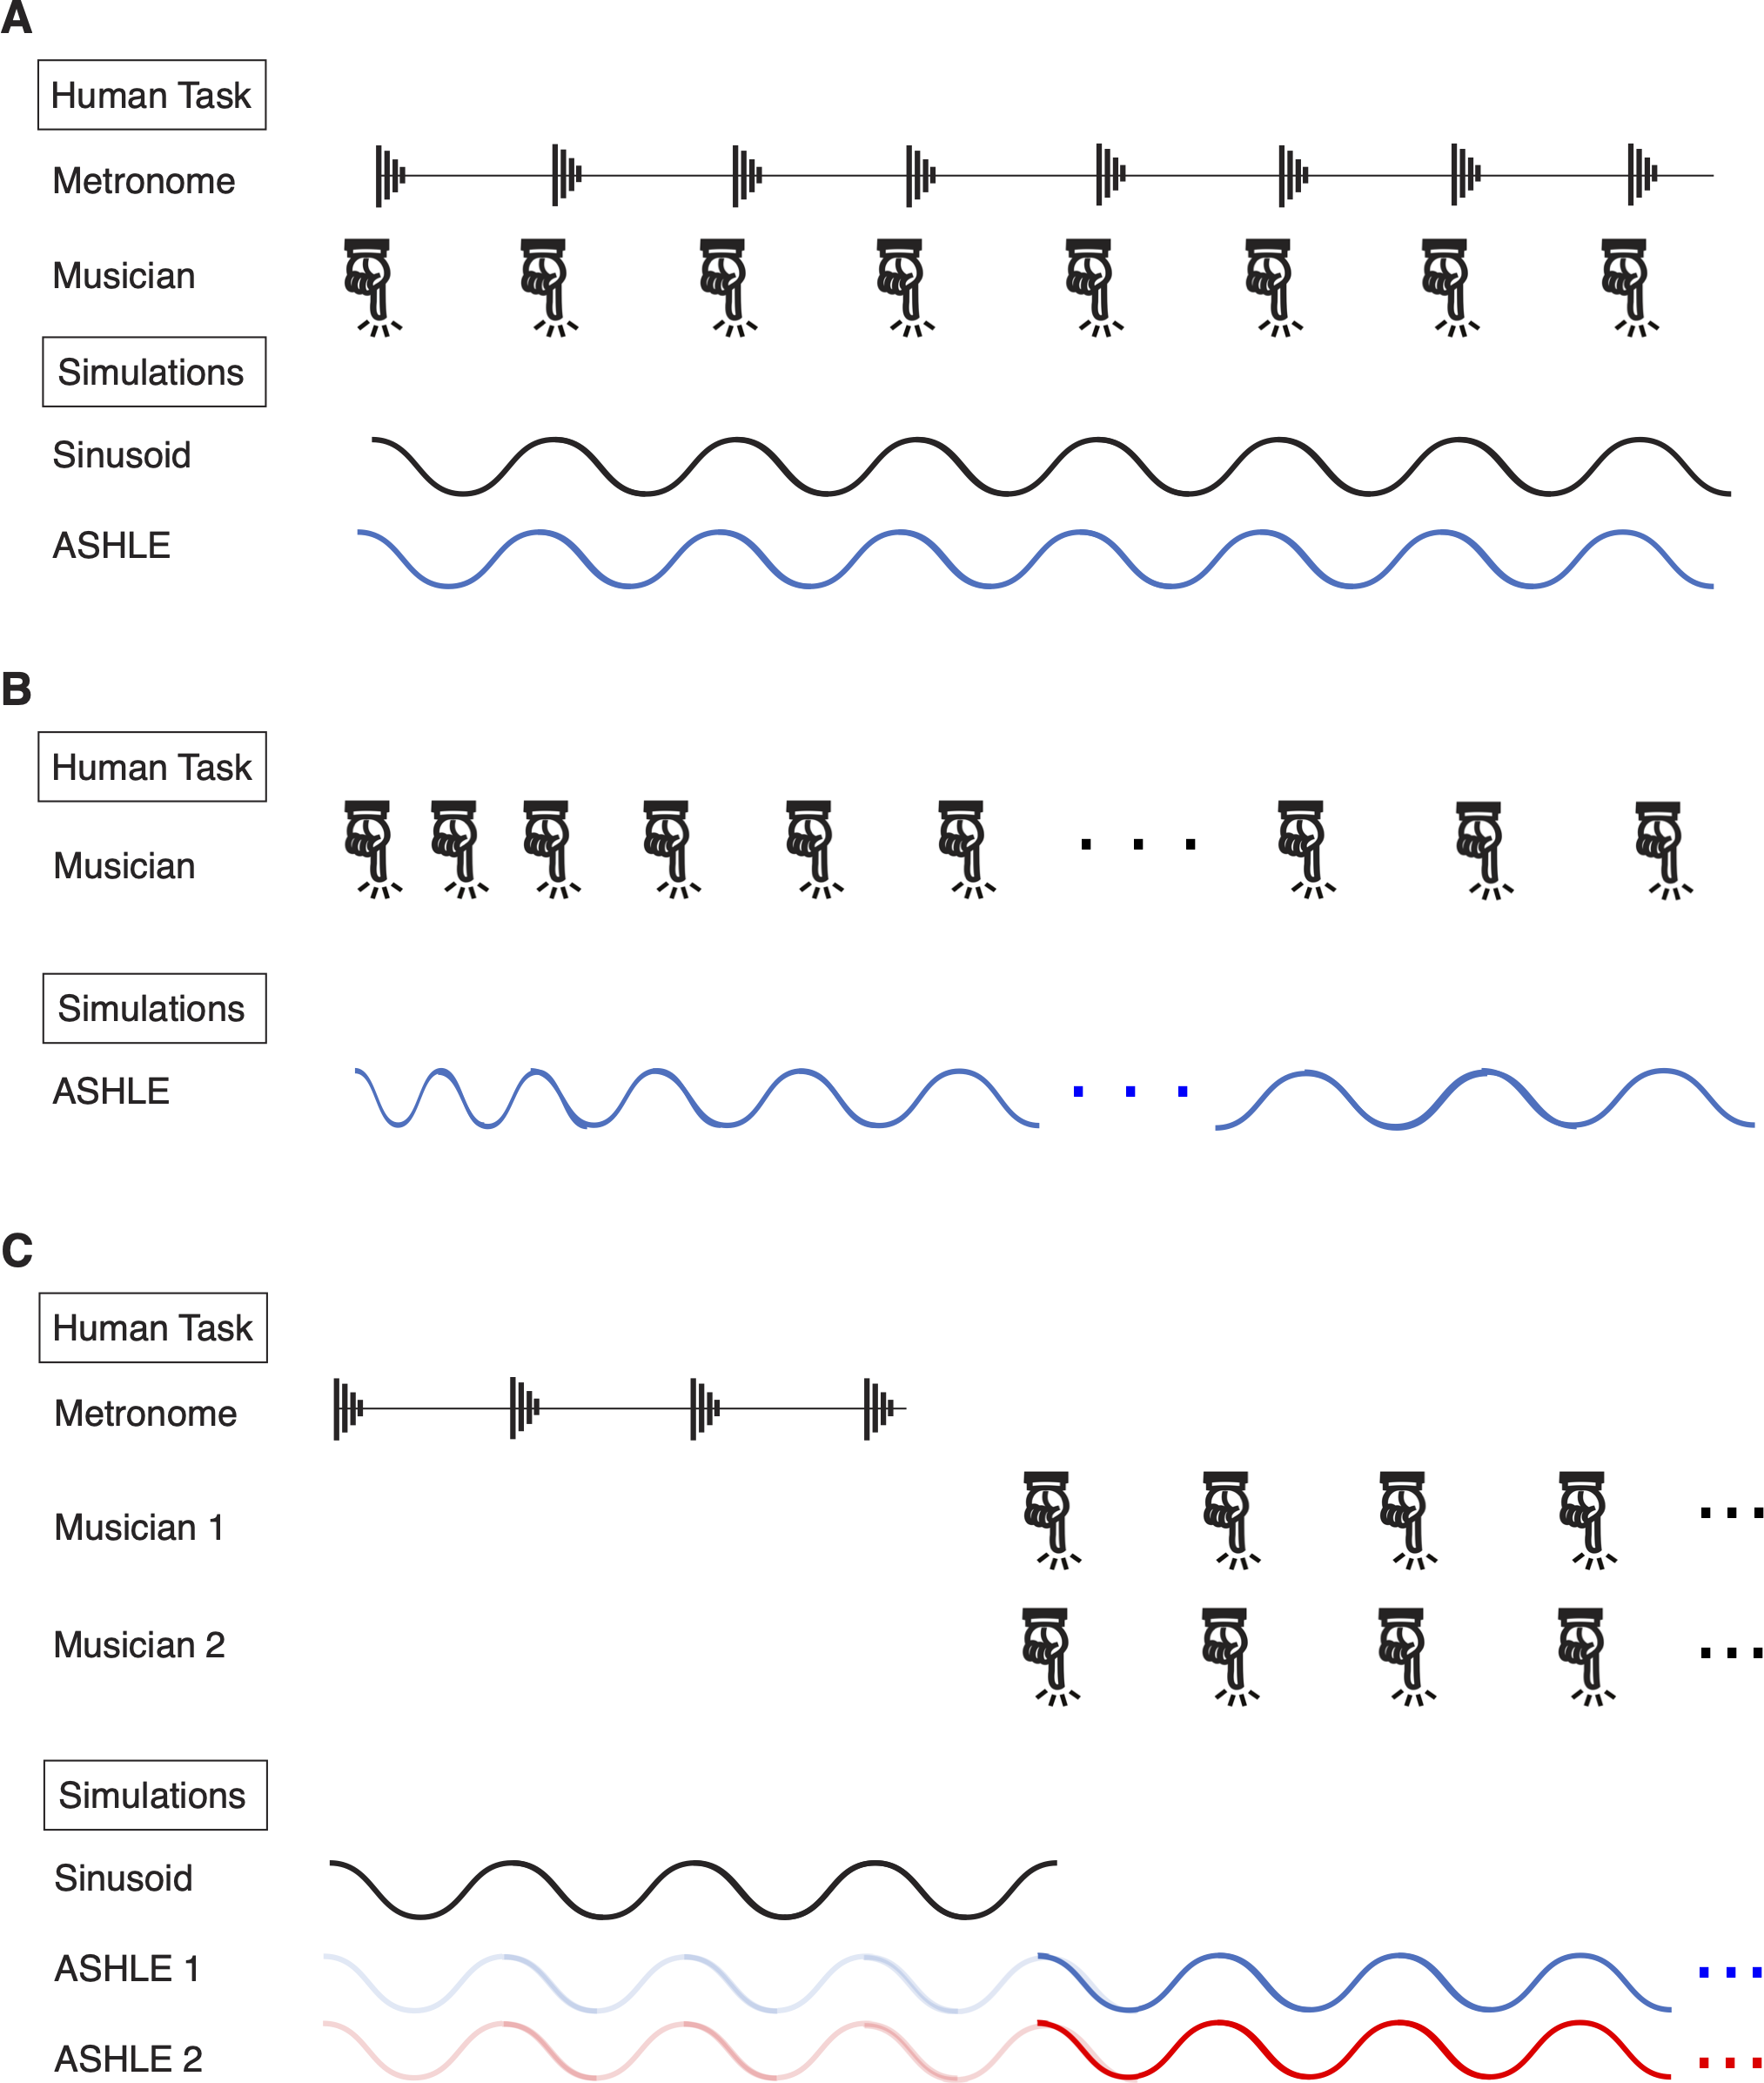
\includegraphics[width=0.9\textwidth]{figures/fig3_1.png}
    \label{f3_1}
\end{figure}
\begin{figure}[t]
    \caption[Illustration of the musical tasks and corresponding simulation experiments]{\textbf{Illustration of the musical tasks and corresponding simulation experiments.} (A) The task simulated in experiment 1, in which a musician plays a simple melody with a metronome (top). In the musician experiment, the metronome tempo was different from the musician's SMT, and we simulate the same experimental conditions. Illustration of our simulation, in which ASHLE synchronizes with a sinusoidal stimulus (bottom). (B) The task simulated in experiment 2, in which a musician plays a simple melody, without a metronome (top). In the musician experiment, musicians started at a tempo that was different from their SMT. This specific example shows a performance that started with a tempo that was faster than the SMT, and the tempo periodically became slower due to the musician's tendency to return to the SMT. Illustration of our simulation, in which ASHLE oscillates, without a sinusoidal stimulus and returns to its natural frequency (bottom). (C) The task stimulated in experiment 3, in which pairs of musicians played a simple melody together after hearing four pacing metronome clicks (top). In the musician experiment, pairs of musicians had matching or mismatching SMTs. Illustration of our simulation, in which two ASHLE models synchronize with four cycles of a pacing sinusoidal stimulus (greyed-out blue and red lines), and then stimulate each other without the sinusoidal stimulus (solid blue and red lines) (bottom).} 
\end{figure}

In our first experiment, we optimized ASHLE to simulate solo musician performance of a simple melody paced by a metronome. This task and data were published by Scheurich and colleagues \cite{scheurich2018tapping}. In this task solo musicians performed a melody with a metronome IOI that was 15\% or 30\% shorter or longer than their SMP (Fig.{} \ref{f3_1}A). Their data showed that the MA grew as a function of the difference between a musician's SMP and the metronome IOI. We simulated this task using ASHLE. We hypothesized that ASHLE's elastic frequency learning will allow for synchronization with stimuli at any arbitrary frequency. Additionally, we hypothesized that the elastic force pulling towards ASHLE's natural frequency will cause the MA between ASHLE and the stimulus to grow as the difference between ASHLE's natural frequency and the stimulus frequency grows.

In our second experiment, we tested whether the same ASHLE model from experiment 1 can simulate solo musician performance of a simple melody without a metronome (unpaced). This task and data were published by Zamm and colleagues \cite{zamm2018musicians}. In this task solo musicians played a melody, without a metronome, starting at five different spontaneous tempi (Fig.{} \ref{f3_1}B). First, at each musician's SMT, then at spontaneous tempi faster and slower than the SMT, and finally at spontaneous tempi that were even faster and even slower than the SMT. Their data showed that when musicians have a tendency to return to their SMT after starting a performance at a tempo faster or slower than their SMT. We hypothesize that our model can simulate the same progressive return to the SMT because of the elastic force constantly pulling ASHLE to its natural frequency. 

In our third experiment, we tested whether the same model from experiments 1 and 2 can simulate duet musician performance of a simple melody. This task and data were published in another study by Zamm and colleagues \cite{zamm2016endogenous}. In this task, pairs of musicians played a melody in synchrony after listening to a metronome that established the tempo and stopped. Musician duets were assigned to either of two experimental groups: duets with matching or mismatching SMTs. The data by Zamm and colleagues \cite{zamm2016endogenous} showed that the mean absolute asynchrony was larger between musicians with mismatching SMTs than musicians with matching SMTs. We hypothesize that ASHLE's elastic frequency learning will allow two of our models to synchronize with each other independent of whether their natural frequencies are close to each other, but that the asynchrony between two different ASHLE models will grow as a function of the difference between their natural frequencies.

These three musician tasks and results capture relationships between the SMT/SMP and the MA. Our goal is to test whether ASHLE's elastic frequency learning can capture these relationships by simulating real musician data. If we are successful, we will shed light on the mechanisms that give rise to the SMT/SMP and the MA. Our model is the first attempt at establishing a mechanistic relationship between the SMT/SMP and the MA that is validated by human data, also making musician data predictions that can be tested empirically in future experiments. Moreover, due to its dynamical systems nature, ASHLE establishes that the SMT/SMP and the MA are related to each other through homeostatic mechanisms at play during PAC.

\section{Results}

\subsection{Experiment 1: Solo music performance with a metronome tempo \\ different than the SMT}

We used ASHLE to simulate the solo task by Scheurich and colleagues \cite{scheurich2018tapping} consisting of music performance of a simple melody paced by a metronome (Fig.{} \ref{f3_1}A). Their experiment had four different experimental conditions: metronome tempo 30\% faster, 15\% faster, 15\% slower, and 30\% slower than the musician's SMT. Fig.{} \ref{f3_2}A shows the data reflecting the mean adjusted asynchrony between the musician beats and the metronome beats across the four different experimental conditions. Scheurich and colleagues \cite{scheurich2018tapping} reported the mean adjusted asynchrony in their results, which is equal to the MA observed during music performance with a metronome tempo different from the musician SMT, minus the MA measured during music performance with an metronome matching the musician SMT (see the methods section for a detailed description of the behavioral task and data). The musician data shows that the mean adjusted asynchrony was positive (negative) when the metronome tempo was faster (slower) than the musicians (SMT), and that the asynchrony grows as a function of the difference between SMT and metronome tempo. While ASHLE does not produce pitch, we can use it to simulate the beats during this music performance task. We hypothesized that ASHLE's tempo learning features will allow it to synchronize with a stimulus faster or slower than its ONT, but an asynchrony between ASHLE and the stimulus will be observed due to the elastic force pulling ASHLE's instantaneous tempo to the ONT. While this first experiment uses a sinusoid to stimulate ASHLE, this contrasts with experiments 2 and 3 described in the next sections, where a sinusoidal stimulus is either completely absent or only present during a brief period at the beginning of the simulation, respectively.

\begin{figure}
    \centering
    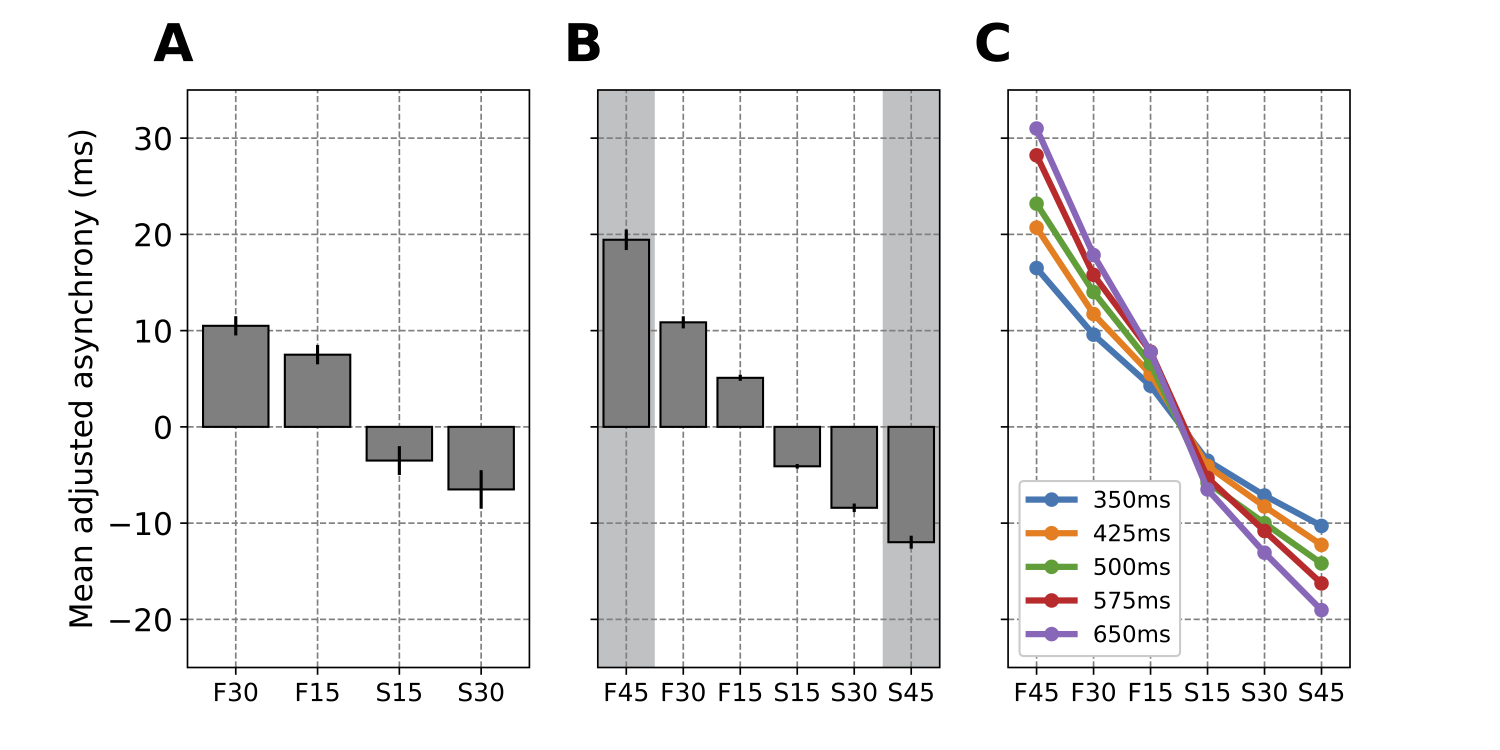
\includegraphics[width=1.0\textwidth]{figures/fig3_2.png}
    \caption[Simulation of the MA between a musician's beat and a metronome beat that is faster or slower than the musician's SMT during solo musical performance]{\textbf{Simulation of the MA between a musician's beat and a metronome beat that is faster or slower than the musician's SMT during solo musical performance.} (A) The mean adjusted asynchrony (and standard error; N=20) between the musician beat and metronome beat during performance of a simple melody in four conditions: metronome tempo 30\% faster, 15\% faster, 15\% slower, and 30\% slower compared to the musician SMT. (B) Our simulation results showing the mean adjusted asynchrony (and standard error; N=20) between ASHLE and a sinusoidal stimulus in six conditions: stimulus tempo 45\% faster, 30\% faster, 15\% faster, 15\% slower, 30\% slower, and 45\% slower compared to ASHLE's ONT. The shaded bars represent predicted measurements for data that has not been collected yet from musicians. (C) Mean adjusted asynchrony predictions when ASHLE models with different ONTs synchronize with a metronome tempo that is 45\% faster, 30\% faster, 15\% faster, 15\% slower, 30\% slower, or 45\% slower than the ONT. The values in (C) are predictions for musician data that has not been collected yet.}
    \label{f3_2}
\end{figure}

We simulated this task using 20 different ASHLE models that differed by their ONT values, which matched each of the 20 musician SMTs measured by Scheurich and colleagues \cite{scheurich2018tapping} (250ms, 260ms, 300ms, 310ms, 325ms, 340ms, 345ms, 350ms, 380ms, 400ms, 410ms, 430ms, 440ms, 450ms, 460ms, 465ms, 475ms, 480ms, 600ms, and 650ms). For each ASHLE model we simulated the task in four experimental conditions where the stimulus tempo was 15\% or 30\% faster or slower than the ONT to measure the asynchrony between ASHLE and the stimulus (see the methods section for details about our simulation setup and procedure). We optimized ASHLE's parameters to approximate the musician data shown in Fig.{} \ref{f3_2}A (see model optimization in the methods section). Fig.{} \ref{f3_2}B shows the mean adjusted asynchrony that we observed in our simulations for the experimental conditions tested by Scheurich and colleagues \cite{scheurich2018tapping}. Our simulations show similar results to the human data observed in Fig.{} \ref{f3_2}A. Additionally, the shaded bars in Fig.{} \ref{f3_2}B show ASHLE's prediction for what the mean adjusted asynchrony would look like if the same group of musicians were to perform with metronome rates 45\% faster or slower than their individual SMT. Our model predicts that the mean adjusted asynchrony in this condition will be even larger compared to when performing with a metronome that is 15\% or 30\% faster or slower than the musician SMT. Fig.{} \ref{f3_2}C shows musician data predictions by simulating different ASHLE models (differentiated by a specific ONT value) that perform the same melody performance task with a metronome tempo that is 45\%, 30\%, and 15\% faster or slower than the ONT. Individual ASHLE models in Fig.{} \ref{f3_2}C predict that the mean adjusted asynchrony grows as a function of the difference between ONT and metronome tempo. Additionally, a longer ONT predicts larger asynchronies across metronome conditions compared to a smaller ONT. The shaded bars in Fig.{} \ref{f3_2}B and the results in Fig.{} \ref{f3_2}C are predictions that ASHLE makes for musician data that has not been collected yet.

Across all 20 ASHLE models simulated in this first experiment, the stimulus was a complex sinusoid $x=\exp(i2\pi f_s t)$, where $f_s$ is a constant dictating the stimulus frequency in hertz, and was different across all simulations (see the methods section for details about the conversion from tempo values to frequency values in hertz for each of the experimental conditions). Each ASHLE model had an ONT value that matched the musician SMT values measured by Scheurich and colleagues \cite{scheurich2018tapping}, which was also the value of ASHLE's initial instantaneous tempo at the beginning of each simulation. The following ASHLE parameters values were always used: $\alpha=1$, $\beta=−1$ ($\alpha$ and $\beta$ are parameters that control ASHLE's oscillatory activity), $\lambda_1=4$ (stimulus tempo learning strength), $\lambda_2=2$ (ONT pulling force), $\gamma=0.02$ (ASHLE's tempo memory leak), and $F=1$ (sinusoidal stimulus force) (see the methods section for a complete mathematical description of the ASHLE model and its parameters). The parameters $\lambda_1$ and $\lambda_2$ act as opposite forces. While $\lambda_1$ allows ASHLE to learn the stimulus tempo, $\lambda_2$ pulls ASHLE to its ONT. Even though $\lambda_1$ is greater in magnitude than $\lambda_2$, they are relatively close, resulting in learning of the stimulus tempo (due to $\lambda_1$) but with an asynchrony between ASHLE and the stimulus (due to $\lambda_2$). In this experiment the parameter $\gamma$ has a negligible effect because of its small value compared to $\lambda_1$, which dominates ASHLE's tempo learning from an external stimulus (see parameter analysis in the methods section for an examination of how different ASHLE parameters values affect its synchronization behavior). Our results show that this set of parameters allows ASHLE to capture the mean adjusted asynchrony values observed in the behavioral data by Scheurich and colleagues \cite{scheurich2018tapping}.

\subsection{Experiment 2: Unpaced solo music performance with a \\ starting tempo different than the SMT}

Experiment 1 showed that our model can capture the MA that Scheurich and colleagues \cite{scheurich2018tapping} observed when musicians individually performed a simple melody paced by a metronome faster or slower than their SMTs. In this second experiment, we used ASHLE to simulate the data by Zamm and colleagues \cite{zamm2018musicians} showing how musicians perform a simple melody without a pacing metronome and spontaneously starting at a tempo different than the SMT (Fig.{} \ref{f3_1}B). Their experiment had four experimental conditions: starting performance tempo fast, faster, slow, and slower than the SMT. Fig.{} \ref{f3_3}A shows their results, which consisted of the adjusted slope across musicians in the four different experimental conditions. The adjusted slope is equal to the slope that best fit the length of consecutive beat IOIs during a melody performance that starts at a tempo different than the SMT, minus the slope that best fit the length of consecutive beat IOIs during a melody performance that starts at the SMT (see the methods section for a detailed description of the task by Zamm and colleagues \cite{zamm2018musicians}). The data shows that when musicians started at a tempo faster than the SMT the mean adjusted was positive (consecutive IOIs became longer), and that when musicians started at a tempo slower than the SMT the mean adjusted slope was negative (consecutive IOIs became smaller). ASHLE does not produce pitch, but we can use it to simulate the beats during this music performance task. We hypothesized that ASHLE's pulling force to the ONT will make it change its oscillation period length to approximate its ONT, but the rate of this change will depend on ASHLE's tempo memory leak (see the methods section for a complete mathematical description of ASHLE). In contrast with experiment 1, in this second experiment ASHLE was never stimulated by a sinusoid. 

\begin{figure}
    \centering
    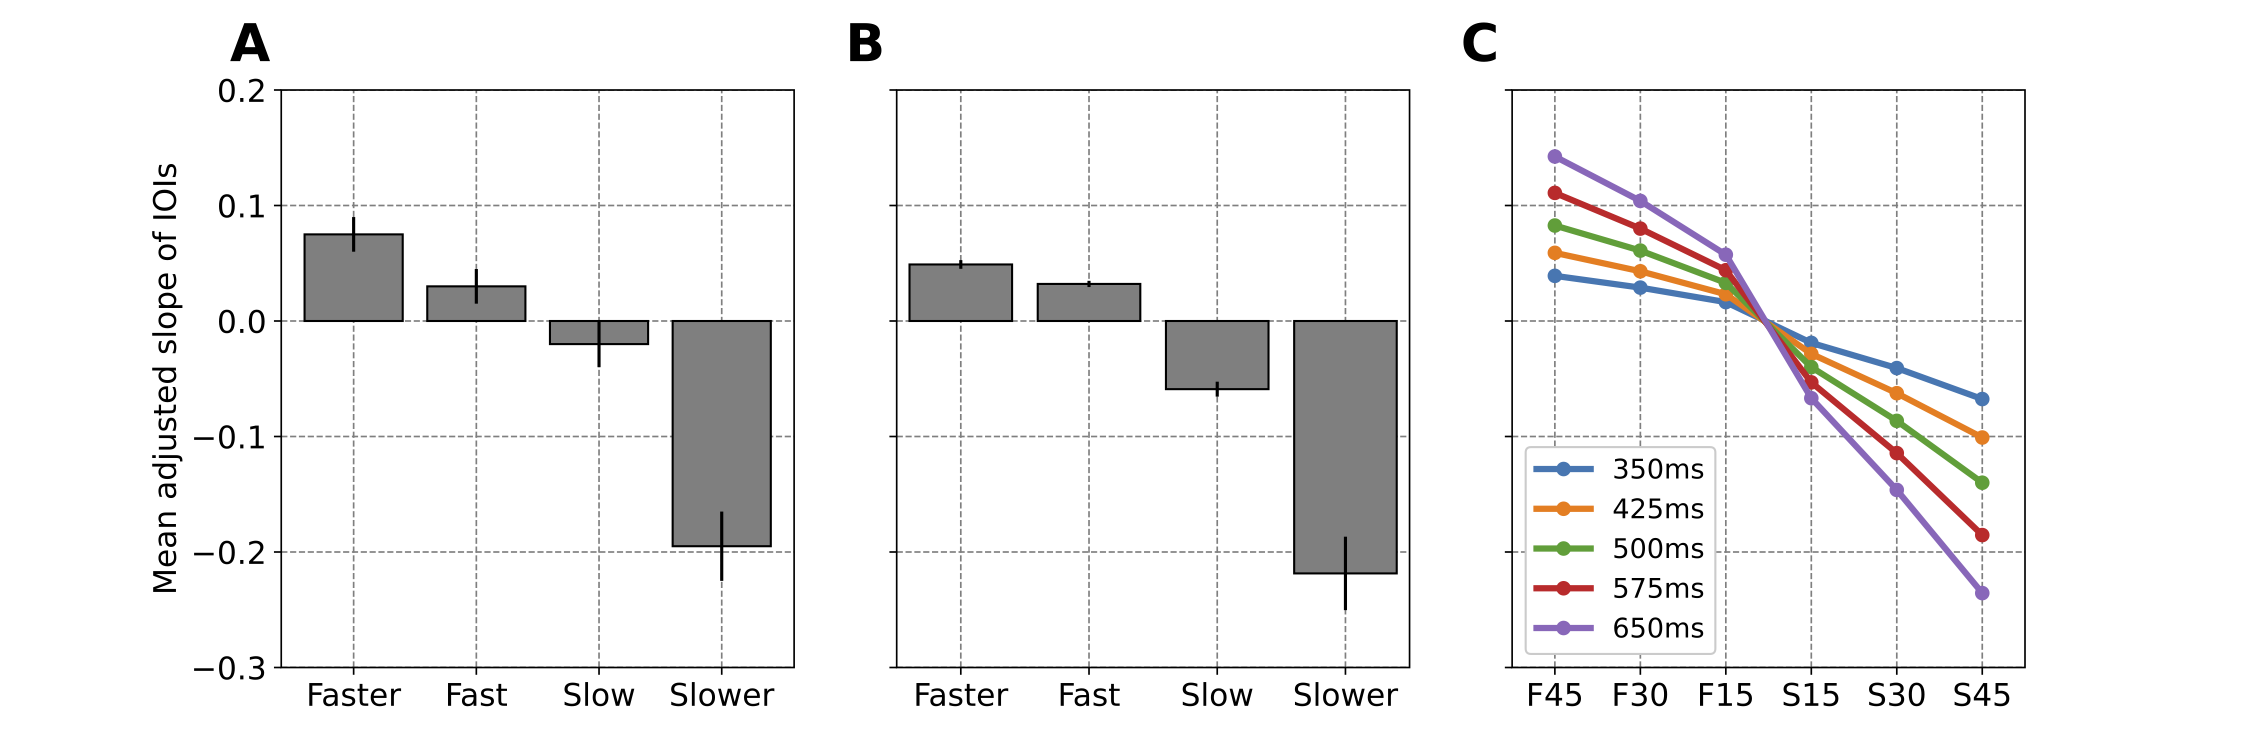
\includegraphics[width=1.0\textwidth]{figures/fig3_3.png}
    \caption[Simulation of the slope between consecutive beat IOIs when an unpaced musician performs a melody starting at a tempo that is different than the SMT]{\textbf{Simulation of the slope between consecutive beat IOIs when an unpaced musician performs a melody starting at a tempo that is different than the SMT.} (A) The mean adjusted slope of consecutive beat IOIs (and standard error; N=24) when solo musicians perform a simple melody starting a tempo that is fast, faster, slow, or slower compared to the musicians SMTs. (B) Our simulation results showing the mean adjusted slope of consecutive beat IOIs (and standard error; N=20) when ASHLE oscillates, without a stimulus, starting at an instantaneous tempo that is fast, faster, slow, or slower compared to the ONT. (C) Adjusted slope predictions when ASHLE models with different ONTs oscillate, without stimulation, starting at an instantaneous tempo value that is 45\% faster, 30\% faster, 15\% faster, 15\% slower, 30\% slower, or 45\% slower compared to ASHLE's ONT. The values in C are predictions for musician data that has not been collected yet.}
    \label{f3_3}
\end{figure}

We simulated this task using 23 ASHLE models that differed by their ONT values, which matched the 23 musician SMT values measured by Zamm and colleagues \cite{zamm2018musicians} (320ms, 350ms, 355ms, 359ms, 382ms, 390ms, 390ms, 415ms, 418ms, 430ms, 435ms, 438ms, 439ms, 439ms, 443ms, 445ms, 455ms, 457ms, 462ms, 470ms, 475ms, 525ms, and 572ms; we excluded the participant with the SMT of 665ms due to the difference between this participants spontaneous rates and the rest of the group; see the methods section for a detailed description of our rationale to exclude this participant). For each ASHLE model we simulated the task in four experimental conditions where ASHLE's initial instantaneous tempo was different: fast, faster, slow, or slower compared to the ONT (see the methods section for details about our simulation setup and procedure). These four initial instantaneous tempo values matched the measurements that Zamm and colleagues \cite{zamm2018musicians} made for each musician performing at a rate that was spontaneously: fast, faster, slow, and slower than the SMT. Fig.{} \ref{f3_3}B shows the adjusted slope that we observed in our simulations for the four different experimental conditions tested by Zamm and colleagues \cite{zamm2018musicians}. Our simulations show similar results to the human data observed in Fig.{} \ref{f3_3}A. Additionally, Fig.{} \ref{f3_3}C shows musician data predictions by simulating different ASHLE models (differentiated by a specific ONT value) that perform the same melody task with an initial instantaneous tempo that is 45\%, 30\%, and 15\% faster or slower than the ONT. Individual ASHLE models in Fig.{} \ref{f3_3}C predict that the slope grows as a function of the difference between initial instantaneous tempo and the ONT. Additionally, a longer ONT predicts larger slope values compared to a smaller ONT. The results in Fig.{} \ref{f3_3}C are predictions that ASHLE makes for musician data that has not been collected yet.

In this second experiment we used the same set of parameter values used in experiment 1. The only values that were different in this experiment were $F = 0$ (due to the lack of stimulus), and the specific ONT and initial tempo values that were dictated by human data. In this experiment $\lambda_1$ is not important to learn the stimulus tempo because there is no stimulus. $lambda_2$ and $\gamma = 0.02$ act as additive forces that control the size of consecutive IOIs in ASHLE's behavior when a stimulus is not present. While $\lambda_2$ dictates how strongly ASHLE pulls its instantaneous tempo towards its ONT, $\gamma$ dictates how strongly ASHLE forgets its instantaneous tempo in favor of the ONT. Here, $\gamma$ is a small value, keeping ASHLE close to its instantaneous tempo and only letting ASHLE slowly return to its ONT due to the pulling force $\lambda_2$. That explains why the resulting slope values in Fig.{} \ref{f3_3}B and \ref{f3_3}C are relatively small (see parameter analysis in the methods section for an examination of how different ASHLE parameters values affect its behavior).

\subsection{Experiment 3: Duet musical performance between musicians \\ with matching or mismatching SMTs}

Experiments 1 and 2 showed that the exact same ASHLE model can simulate two different behavioral measurements: the MA in paced musical performance and the slope of consecutive IOIs in unpaced musical performance. In this third experiment, we used ASHLE to simulate another task by Zamm and colleagues \cite{zamm2016endogenous} showing how musician duets perform a simple melody four consecutive times (Fig.{} \ref{f3_1}C). Musician duets were separated into two experimental groups: pairs with matching or mismatching SMTs. Fig.{} \ref{f3_4}A shows their results, which consisted of the mean absolute asynchrony between the beats of the two performing musicians in each of the two experimental groups, separately for each of the four melody repetitions (see the methods section for a detailed description of the task by Zamm and colleagues \cite{zamm2016endogenous}). This data shows that the mean absolute asynchrony was smaller between musician duets with matching SMTs compared musician duets with mismatching SMTs. ASHLE does not produce pitch, but we can use it to simulate the beats during this musical performance task. We hypothesized that two ASHLE models will be able to synchronize with each other due to their tempo learning mechanism, but the elasticity pulling to their respective ONT will result in asynchrony between them, and that the asynchrony will be smaller between two synchronizing ASHLE models with similar ONT values compared to two ASHLE models dissimilar ONT values. In this third experiment pairs of ASHLE models are stimulated first by a sinusoid that establishes a common tempo and then the two ASHLE models stimulate each other. As a result, stimulation in this third experiment is overall more complex than the constant sinusoidal stimulation in experiment 1 and the lack of stimulation in experiment 2.


\begin{figure}
    \centering
    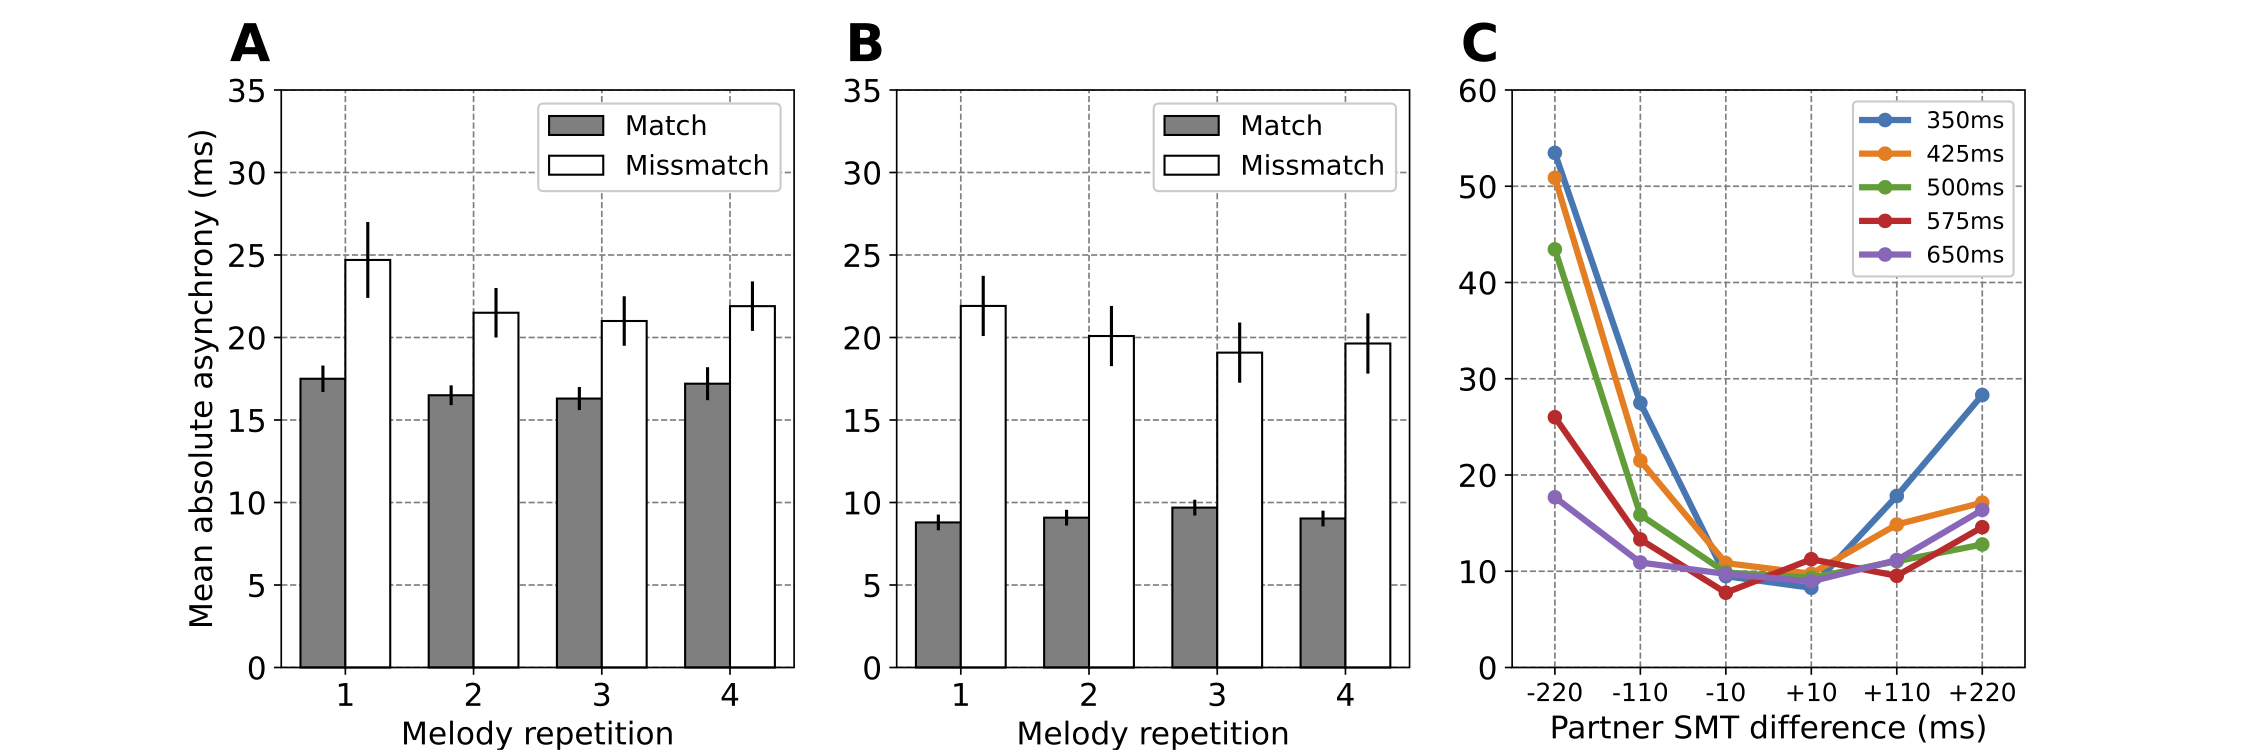
\includegraphics[width=1.0\textwidth]{figures/fig3_4.png}
    \caption[Simulation of the mean absolute asynchrony between two musicians with matching or mismatching SMTs during duet musical performance]{\textbf{Simulation of the mean absolute asynchrony between two musicians with matching or mismatching SMTs during duet musical performance.} (A) The mean absolute asynchrony (and standard error; N=10 in each experimental group) between two musicians with matching or mismatching SMTs during performance of a simple melody four consecutive times. (B) Our simulation results showing the mean absolute asynchrony between two synchronizing ASHLE models with matching or mismatching ONTs. (C) Mean absolute asynchrony predictions when ASHLE models with different ONT values synchronize with another ASHLE model with an ONT that is 220ms shorter, 110ms shorter, 10ms shorter, 10ms faster, 110ms faster, and 220ms faster. The values in C are predictions for data that has not been collected yet from musicians.}
    \label{f3_4}
\end{figure}

We simulated this task using 40 ASHLE models that differed by their ONT values, which matched each of the 40 musician SMT values measured by Zamm and colleagues \cite{zamm2016endogenous}. We paired ASHLE models replicating Zamm and colleagues' \cite{zamm2016endogenous} pairing of musicians with matching or mismatching SMTs. For each pair we simulated the duet melody performance task, where musician duets performed the same simple melody four consecutive times (see the methods section for details about our simulation setup and procedure). We used the same ASHLE parameters that we used in experiments 1 (except for $F_z = 0.01$ when ASHLE models stimulated each other, and the addition of gaussian noise to ASHLE's effector to better approximate the musician absolute asynchrony magnitudes in duet performance; see model optimization in the methods section). Fig.{} \ref{f3_4}B shows the mean absolute asynchrony that we observed in our simulations for the experimental groups and melody repetitions tested by Zamm and colleagues \cite{zamm2016endogenous}. Our simulations show similar results to the human data observed in Fig.{} \ref{f3_4}A. Additionally, Fig.{} \ref{f3_4}C shows musician data predictions by simulating different ASHLE models (differentiated by a specific ONT value) performing the same duet melody task paired with another ASHLE model that has an ONT 220ms shorter, 110ms shorter, 10ms shorter, 10ms faster, 110ms faster, and 220ms faster. Individual ASHLE models in Fig.{} \ref{f3_4}C predict that the mean absolute asynchrony between musician pairs grows as a function of the difference between their ONT values. 

In this third experiment we used the same set of parameter values used in experiments 1 and 2, except for the ONT values, which were dictated by human data. However, stimulation of ASHLE models was different and more complex compared to the experiments 1 and 2. First, in the same way as in experiment 1, the two ASHLE models simulating duet performance were stimulated by four cycles of a sinusoid (with a period length of 400ms and $F = 1$) to establish a common performance beat. Then, the two ASHLE models stimulated each other for the rest of the simulation with an $F_z = 0.01$, which is considerably smaller when two ASHLE models stimulate each other in order to control the stability of synchronization (see model optimization in the methods section). Additionally, we added gaussian noise $\mathcal{N}(\mu=0, \sigma^2=100)$ to ASHLE's effector to better approximate the musician duet performance data. Without the gaussian noise, ASHLE showed the same relative difference in the mean absolute asynchrony between experimental groups (match or mismatch SMT), but the values were considerably smaller (see  model optimization in the methods section).

\section{Discussion}

\subsection{The interaction of Hebbian learning and elasticity mechanisms \\ during beat tracking can capture various PAC behaviors}

The asynchrony between ASHLE and a periodic stimulus was modulated using a tempo learning rule with an elastic force. Similarly, in the absence of a stimulus the tempo learning and the elastic force also affected the changes in cycle length in ASHLE's spontaneous activity, especially if ASHLE's instantaneous tempo was different than its ONT (see parameter analysis in the methods section). ASHLE's behavior is the result of the tempo learning and the elastic force, which act in opposite directions. While Hebbian tempo learning lets ASHLE change its instantaneous tempo to perfectly match any stimulus tempo value, the elastic force pulls ASHLE to its ONT. ASHLE's behavior is consistent with theoretical accounts highlighting that a systems natural tempo (or natural frequency) is the optimal state for synchronization, even if the system can adapt to synchronize at other frequencies \cite{von1937nature, haken1985theoretical, kelso1997relative, scheurich2018tapping}. An interesting question is where in the musician brain these mechanisms of tempo learning and ONT elasticity occur. As far as tempo learning, previous research shows that cortical and subcortical networks in motor brain areas synchronize neural activity that reflects the rhythms of a periodic stimulus \cite{large2015neural, chen2008moving, grahn2009feeling, fujioka2012internalized}. The origins of the SMT in humans (simuated by ASHLE's ONT) involve both the central and the peripheral nervous system. Central pattern generators in the central nervous system give rise to spontaneous rhythms that could directly control the SMT \cite{latash1992virtual}. Additionally, production of SMTs involves the actions of effectors (i.e., foot or fingers), so anatomical and biomechanical factors could also directly contribute to defining a system's SMT \cite{goodman2000advantages}. Currently no consensus exists about the origins of the SMT and its influence during PAC. ASHLE is the first model validated by real human data that captures how the brain's motor system entrains to the tempo of a periodic stimulus and is influenced by the dynamic principles of Hebbian tempo learning and SMT elasticity that give rise to the SMT.

\subsection{Experiment 1: Solo music performance with a metronome tempo \\ different than the SMT}

Our model was able to reproduce the mean adjusted asynchrony between musician beats and metronome beats that are faster or slower than the musician's SMT, in a simple musical performance task (Figs \ref{f3_2}A and \ref{f3_2}B). Taking a closer look at the behavioral data in Fig.{} \ref{f3_2}A we see that the magnitude of the mean adjusted asynchrony values is slightly asymmetric between faster and slower stimuli with respect to the SMT, with faster metronomes resulting in slightly larger mean adjusted asynchrony magnitudes than slower ones. To achieve this behavior in ASHLE we had to frequency-scale the adaptive and elastic stimulus tempo learning rules controlled by $\lambda_1$ and $\lambda_2$ parameters, respectively, in Eqs \eqref{eq:3.6} and \eqref{eq:3.8} (see \cite{kim2015signal, large2010canonical} for more theory about frequency-scaled dynamical systems similar to ASHLE). Additionally, ASHLE's elasticity term $-\lambda_2\left(\exp\left(\frac{f_m-f_0}{f_0}\right)-1\right)$ in Eq \eqref{eq:3.8} is an exponential function so that a stimulus faster than ASHLE's ONT (causing $\exp\left(\frac{f_m-f_0}{f_0}\right)-1>0$) would result in an exponentially larger force toward the ONT compared to a stimulus slower than ASHLE's ONT (causing $\exp\left(\frac{f_m-f_0}{f_0}\right)-1<0$). Due to frequency scaling, higher instantaneous values of $f_e$ and $f_m$ amplify the tempo learning rate ($\lambda_1$) and the elastic force pulling to ASHLE's ONT ($\lambda_2$), while lower instantaneous $f_e$ and $f_m$ values shrink $\lambda_1$ and $\lambda_2$. In ASHLE $f_e$ and $f_m$ are always very close (if not identical) in value to each other. ASHLE's mechanisms and behavior are validated by its ability to simulate the data by Scheurich and colleagues \cite{scheurich2018tapping} (Fig.{} \ref{f3_2}A and \ref{f3_2}B).

ASHLE's mechanisms of tempo adaptation and elastic force pulling to the ONT can also be neuroscientifically explained. ASHLE's $\lambda_1$ parameter for tempo adaption simulates the brain's ability to entrain cortical and subcortical motor networks when processing a periodic temporal stimulus like a musical beat or a metronome tempo \cite{large2015neural}. In contrast, ASHLE's $\lambda_2$ parameter simulates the stiffness of the human body's anatomical and biomechanical properties that give rise to the SMT \cite{goodman2000advantages}

While ASHLE was able to simulate the musician data by Scheurich and colleagues \cite{scheurich2018tapping}, it does not show variability in its dynamics. Once ASHLE phase-locks with the sinusoidal stimulus, the asynchrony between ASHLE and the stimulus reaches a steady state with zero variability. This is a limitation of ASHLE's ability to simulate musician's beat tracking behavior, reflected by a degree of variability across musician beat IOIs. In experiment 1, this lack of variability was a limitation to perfectly simulate the results by Scheurich and colleagues \cite{scheurich2018tapping}. Using ASHLE with different ONT values allowed us to simulate the variability between musicians (hence the standard error in Fig.{} \ref{f3_2}B). However, our standard errors were overall smaller compared to the musician standard errors that Scheurich and colleagues \cite{scheurich2018tapping} reported. The standard error in musicians has two sources: (1) variability within each musician's beat tracking behavior and (2) variability between the behavior of different musicians. While we were able to simulate the variability between musicians using ASHLE models with different ONT values, the lack of noise in ASHLE's activity is the likely cause of the difference between our simulation results and the musician results. Adding gaussian noise to ASHLE's activity could better approximate the musician results. However, we considered the addition of noise to be beyond the scope of this first experiment because our goal was to optimize ASHLE to simulate the magnitude of the mean adjusted asynchrony (see model optimization in the methods section).

ASHLE also made testable predictions of paced musician performance in a solo setting (Figs \ref{f3_2}B and \ref{f3_2}C). First, it predicted mean adjusted asynchrony values that we could expect if the same group of musicians were to carry out the task synchronizing with a metronome 45\% faster or slower than the SMT (Fig.{} \ref{f3_2}B shaded bars). Additionally, Fig.{} \ref{f3_2}C made predictions at the individual musician level, simulating the mean adjusted asynchronies that musicians with different SMT would produce when performing a melody with various metronome tempi faster or slower than the SMT. ASHLE can be used to make predictions about a musician with any SMT, and such predictions can be empirically tested to further validate ASHLE's behavior.

\subsection{Experiment 2: Unpaced solo music performance with a \\ starting tempo different than the SMT}

Our model was also able to simulate the mean adjusted slope between consecutive IOIs that Zamm and colleagues \cite{zamm2018musicians} observed when musicians performed a melody without a metronome, starting at a tempo faster or slower than the SMT (Figs \ref{f3_3}A and \ref{f3_3}B). ASHLE's approximation of the data is not perfect, but it is close. This is because the parameters $\lambda_1$ and $\lambda_2$ were optimized to simulate the data in experiment 1 and the same values were used in experiment 2. Hence, our results in this second experiment show that the values for $\lambda_1$ and $\lambda_2$ can generalize to simulate data across different musician datasets. There was only one ASHLE parameter that we optimized based on the musician data from experiment 2. This was the $\gamma$ parameter (see model optimization of experiment 2 in the methods section). In experiment 2 there is no sinusoidal stimulus ($F=0$) and $\gamma$ in Eq \eqref{eq:3.5} controls how quickly ASHLE forgets its instantaneous tempo in favor of the ONT. $\gamma = 0.02$ was the value that resulted in the best fit between ASHLE's simulation results and the musician data results. The small $\gamma=0.02$ value can be explained by looking at the musician data in Fig.{} \ref{f3_3}A. Musician's mean adjusted slope values are relatively small for all experimental conditions. These small values result from musicians showing a tendency to very slowly return to their SMT throughout the musical performance. That is why the value of $\gamma$ is very small compared to $\lambda_1=4$ and $\lambda_2=2$. Hence, $\gamma$ is the ASHLE parameter that represents a musician's tendency to return to their SMT in the absence of stimulation and it is relatively small because part of musical training consists in being able to maintain an arbitrary tempo throughout a musical performance \cite{fine2009memory, schultz2019roles}.

Theoretical models of musical tempo suggest entrainment of periodic neural activity with periodic actions \cite{large1999dynamics}, but the mean adjusted slope results by Zamm and colleagues \cite{zamm2018musicians} also suggests that the motor system, while maintaining the musical tempo, is constantly influenced by the biomechanical properties that give rise to the SMT \cite{goodman2000advantages}. Evidence from synchronization-continuation tasks suggest the existence of a physical and likely anatomical force pulling human periodic actions to the SMT in the absence of an external stimulus \cite{yu2003task, mcauley2006time}. Our simulations reflect that the same mechanisms to maintaint a tempo are at play in experiment 1 and 2. However, the presence of a stimulus in experiment 1 resulted in maintaining the tempo and the observation of an MA between the musician and the metronome. In contrast, the lack of stimulus in experiment 2 results in the musician slowly returning to the SMT.

Like in experiment 1, in experiment 2 ASHLE lacks variability in its activity. The standard errors in our simulation results (Fig.{} \ref{f3_3}B) are different to the standard errors in the musician results (Fig.{} \ref{f3_3}A). As we discussed in experiment 1, the musician results have two sources of activity: variability in each individual musician's actions and variability between musicians. Our simulations only capture the variability between musicians by using different ONT values to simulate different musician's SMTs. ASHLE's lack of variability in its activity suggest that the variability in each individual musician's actions contributes to the standard error observed in Fig.{} \ref{f3_3}. Our simulations of experiment 2 show that ASHLE is a good model to approximate the slope but not the variability observed between musicians that try to maintain the tempo in a solo setting without a pacing metronome.

ASHLE also made testable predictions of unpaced musician performance in a solo setting. Fig.{} \ref{f3_3}C shows predictions at the individual musician level simulating the mean adjusted slope that musicians with different SMT would produce when performing a melody starting at various tempi that are faster or slower than the SMT. ASHLE can be used to make predictions about a musician with any SMT, and such predictions can be empirically tested to further validate ASHLE's behavior.

\subsection{Experiment 3: Duet musical performance between musicians \\ with matching or mismatching SMTs}

ASHLE was able to simulate the mean absolute asynchrony between the beat of duets of musicians (with matching or mismatching SMTs) that performed a simple melody (Fig.{} \ref{f3_4}A and \ref{f3_4}B). With the exception of the type of stimulation (which was different between all three experiments) we used the same ASHLE model parameters in experiments 1, 2, and 3. By carrying out experiment 3, our goal was to show that ASHLE can capture musical performance behavior not just in solo settings, but also in a duet setting. To optimize ASHLE for experiment 3, we added noise to ASHLE's effector (see model optimization in the methods section). Without this noise, ASHLE's simulation of experiment 3 reflected some of the general trends in the musician results, but with a noticeable difference in magnitude between the musician mean absolute asynchrony and ASHLE's (see Fig.{} \ref{f3_5}). Adding noise to ASHLE's effector significantly improved ASHLE's approximation of the human data (Figs \ref{f3_4}A and \ref{f3_4}B). More specifically, the added noise results in ASHLE approximating the magnitude of the mean absolute asynchrony in the musician duets with mismatching SMTs and marginally approximating the results of musician duets with matching SMTs. Across all simulations, the standard error in ASHLE's results is very similar to the standard error displayed by the human data. While we could have changed parameter values to achieve a perfect match between ASHLE's simulations and the musician activity for all experimental conditions, our goal was to identify the best set of parameter values that could capture the activity across different musician experiments.

\begin{figure}
    \centering
    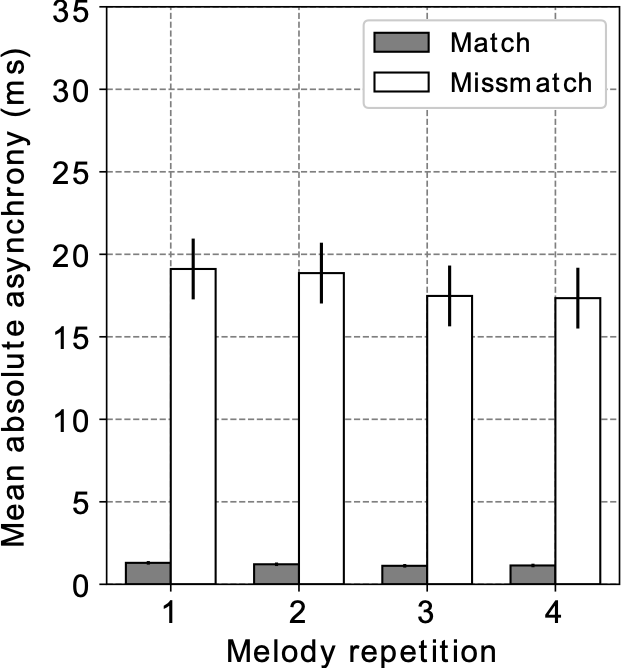
\includegraphics[width=0.5\textwidth]{figures/fig3_5.png}
    \caption[Simulation without noise of the mean absolute asynchrony between two musicians with matching or mismatching SMTs during duet musical performance]{\textbf{Simulation without noise of the mean absolute asynchrony between two musicians with matching or mismatching SMTs during duet musical performance.} Our simulation results showing the mean absolute asynchrony between two synchronizing ASHLE models with matching or mismatching ONTs, but no noise is added to Eq \eqref{eq:3.7}. The resulting mean absolute asynchronies in this simulation without noise are much smaller compared to the musician data results in Fig.{} \ref{f3_4}A. The added noise in Eq \eqref{eq:3.9} improves the model's results, which are shown in Fig.{} \ref{f3_4}B.}
    \label{f3_5}
\end{figure}

ASHLE was able to simulate the solo performance results in experiments 1 and 2 without the need of noise. However, noise was necessary to simulate the duet performance results in experiment 3. This makes sense as the musical performance task in experiment 3 involves more sources of variability than the tasks in experiments 1 and 2. While only one musician performs in experiments 1 and 2, in experiment 3 there are two performing musicians receiving feedback from each other. The variability in musician behavior noticeably influences the absolute asynchrony between two musicians performing as a duet. ASHLE's need for noise in its effector term $z_m$ reveals that the variability in musician behavior at the individual level is a significant contributor to the mean absolute asynchrony in experiment 3. Without noise, ASHLE simulated a mean absolute asynchrony around 2ms and 18ms for the duets with matching and mismatching SMTs, respectively. When noise was added, ASHLE simulated a mean absolute asynchrony around 10ms and 20ms for the duets with matching and mismatching SMTs, respectively. Hence, the presence of noise is needed to capture musical duet behavior, especially when the two musicians have matching SMTs.

To simulate this musical duet task, we also needed a significantly smaller connection strength (see model optimization in the methods section) between the two ASHLE models stimulating each other. This difference in stimulus strength between experiment 1 and experiment 3 is due to the nature of the stimulus. When the stimulus lacks intrinsic dynamical properties, like the sinusoidal stimulus in experiment 1, a large forcing strength helps achieving phase-locked synchronization between a dynamical system and the sinusoid \cite{kim2015signal}. This is very different when two or more dynamical systems stimulate each other, like the two ASHLE models stimulating each other in experiment 3. Previous studies of stability between dynamical systems have revealed that small forcing strengths between dynamical systems ensure the stability of their periodic behavior \cite{kim2015signal}.

ASHLE also made testable predictions about how musician duets would perform. Fig.{} \ref{f3_4}C shows predictions for the mean absolute asynchrony that one would observe between two musicians, one with a specific SMT, and the other with an SMT that differs by a specific value from the other musician's SMT. These predictions show that the mean absolute asynchrony between the two musicians will generally vary as a function of the difference between the musician's SMTs, and also as a function of the specific SMT value in either of the two musicians. ASHLE can be used to make predictions about musician duets with any SMTs, and such predictions can be empirically tested to further validate ASHLE's behavior.

\subsection{General discussion}
We have presented the ASHLE model, which captures how the musical tempo is maintained during various simple performance tasks. In experiment 1, ASHLE captured the MA between a musician's beats and metronome beats during a simple melody performance task (Fig.{} \ref{f3_2}). In experiment 2, ASHLE captured the rate of beat change when a solo musician performed a simple melody without a metronome (Fig.{} \ref{f3_3}). And in experiment 3, ASHLE captured the mean absolute asynchrony between the beat of two musicians performing a simple melody as a duet (Fig.{} \ref{f3_4}). ASHLE was able to capture these three different tasks using the same set of parameters for its intrinsic dynamics (see parameter analysis and model optimization in the methods section). Our simulations validate ASHLE's ability to simulate real musician data. Hence, ASHLE is a model with mechanisms of adaptive and elastic tempo tracking that generalize across different tasks, different musicians, and different datasets. We also used ASHLE to make testable predictions of musician performance data not yet collected (Figs \ref{f3_2}B, \ref{f3_2}C, \ref{f3_3}C, and \ref{f3_4}C). Future behavioral studies can collect this data to validate ASHLE as a model able to capture musician performance. More data collected could also help to better fine tune ASHLE's parameters in case ASHLE, in its current sate, cannot sufficiently predict new musician data.

ASHLE is the first MA model with the interacting forces of Hebbian tempo learning and elasticity pulling toward a systems natural tempo. Previous models have focused on explaining the origin of the negative mean asynchrony (NMA), which is a specific type of MA when the synchronizing agent's actions anticipate the pacing signal (i.e., a metronome). The first kind of these models propose that the NMA is the result of adaptive synchronization by means of phase and period correction rules at phenomenological \cite{van2013adaptation} and neuromechanistic levels \cite{bose2019neuromechanistic}. Another kind of models, called strong anticipation models, propose that the NMA is the result of delayed feedback \cite{stepp2010strong} and, in the case of humans, the NMA has been theorized to emerge from delayed neural communication in the sensorimotor system \cite{roman2019delayed}. ASHLE can capture both the NMA and the positive MA using the same fundamental principles of adaptive tempo learning and elastic forces pulling to a system's natural tempo. In humans, the NMA is observed when synchronizing with a metronome tempo with an IOI larger than 350ms \cite{mates1994temporal}. Interestingly, the average human SMT is around 400ms. As a result, the human NMA in ASHLE emerges from a force pulling the human tempo to the SMT during adaptive synchronization with a slower stimulus. However, there are similarities between ASHLE and models of strong anticipation to explain the NMA as resulting from delayed feedback \cite{stepp2010strong, roman2019delayed}. Both ASHLE and strong anticipation models are based on physical principles. Future work should try to combine ASHLE and the strong anticipation model of human anticipation to achieve a comprehensive model of adaptive and anticipatory activity in human behavior.

We have presented a versatile, neuroscientifically-inspired, and ecologically valid model of adaptive musical beat performance for solo and duet settings. ASHLE is a model that can capture adaptive human synchronization based on dynamical principles. ASHLE could be used not just to simulate human data and predict human behavior, but also as a tool with which humans can interact in experimental, musical, and therapy settings. In general, ASHLE is the first model of its kind, and provides us with a better understanding about how Hebbian tempo learning in the motor cortex interacts with the elastic and dynamical constraints that give rise to the SMT.

\section{Methods}

\subsection{Model definition}

\subsubsection{Theoretical background}

A non-linear oscillator with an ONT (or natural frequency) $f_1$ can synchronize in a phase-locking fashion with another oscillator or an arbitrary periodic signal of tempo $f_2$ if $|f_1 − f_2| < \epsilon$, where $\epsilon$ is much smaller compared to $f_1$ and $f_2$. Synchronization also requires the synchronizing oscillator (or oscillators) to have properly defined parameter values because if any of these parameters is outside the oscillator's phase-locking regime, synchronization will fail \cite{righetti2006dynamic}. To overcome the limitation of fixed parameters, studies have shown that oscillator parameters can be defined dynamically by a differential equation \cite{acebron1998adaptive, borisyuk2001oscillatory, ermentrout1991adaptive, nakanishi2003learning, nishii1999learning, righetti2006dynamic}. Because the tempo term is critical to determine an oscillator's phase-locking regime, Righetti and colleagues \cite{righetti2006dynamic} defined an equation that allows a limit-cycle oscillator to dynamically adapt its tempo to match the rate of periodic activity of an arbitrary stimulus and phase-lock.

\begin{equation}
\dot{f} = -\lambda x(t) \sin(\phi) \label{eq:3.1}
\end{equation}

In Eq \eqref{eq:3.1}, $f$ is an oscillator's ONT (or natural frequency) in hertz, $\lambda$ is the learning rate (or the adaptation timescale for $f$), $x(t)$ is an arbitrary stimulus, and $\phi$ is the oscillator's instantaneous phase \cite{righetti2006dynamic}. Because $f$ is a real-valued term, the stimulus $x(t)$ is assumed to be a real signal, but if it were complex-valued, only the real part of $x(t)$ would be needed to observe the adaptive tempo behavior. Hence, to process a complex-valued stimulus, Eq \eqref{eq:3.1} would have the following form:

\begin{equation}
\dot{f} = -\lambda \Re \{ x(t) \sin(\phi) \} \label{eq:3.2}
\end{equation}

Eq \eqref{eq:3.2} allows a non-linear oscillator to dynamically adapt its tempo to phase-lock with a periodic stimulus (real- or complex-valued) of an arbitrary tempo \cite{righetti2006dynamic}. However, Eq \eqref{eq:3.2} does not have memory, so after stimulation the oscillator's tempo $f$ will remain in its learned state and will not return to the oscillator's original ONT. Lambert and colleagues \cite{lambert2016adaptive} envisioned an oscillator able to adapt its tempo elastically so that the oscillator would return to its ONT in the absence of stimulation. Eq \eqref{eq:3.3} describes this elastic tempo learning rule:

\begin{equation}
\dot{f} = -\lambda_1 \Re \{ x(t) \sin(\phi) \} - \lambda_2 \frac{f-f_0}{f_0} \label{eq:3.3}
\end{equation}

In Eq \eqref{eq:3.3}, $\lambda_1$ is the tempo learning rate from Eq \eqref{eq:3.2} and $\lambda_2$ is the elastic force pulling the oscillator's $f$ back to $f_0$, which is a fixed value representing the oscillator's ONT. $\lambda_2$ multiplies the difference between $f$ and $f_0$. Thus, the new term $−\lambda_2 \frac{f-f_0}{f_0}$ is equivalent to Hooke's law, which states that the force needed to extend a spring is linearly scaled by the distance resulting from such extension \cite{lambert2016adaptive}. As $f$ and $f_0$ differ in value due to a stimulus $x(t)$ that changes the adaptive tempo term $-\lambda_1 \Re \{ x(t) \sin(\phi) \}$, the system's elastic energy demand increases. Only the stimulus $x(t)$ can supply this energy demand, and in the absence of a stimulus, the system will make $f = f_0$, which is the state with the lowest elastic energy demand. Lambert and colleagues \cite{lambert2016adaptive} used Eq \eqref{eq:3.3} to create networks of oscillators with different $f_0$ values. This network allowed them to dynamically find pulse and meter in musical signals \cite{lambert2016adaptive}.

To use Eq \eqref{eq:3.3} we need to combine it with an oscillatory dynamical system. Because we want to simulate periodic synchronization, we use the canonical Hopf oscillator described by Large and colleagues that can synchronize with an external periodic stimulus \cite{large2010canonical, kim2015signal}. The oscillator that we will use has the following general form:

\begin{equation}
\frac{1}{f}\dot{z} = z\bigg(\alpha + i2\pi + \beta_1|z|^2 + \frac{\epsilon\beta_2|z|^4}{1-\epsilon|z|^2}\bigg) + x(t) \label{eq:3.4}
\end{equation}

In Eq \eqref{eq:3.4} $z$ is the state of the oscillator, and $\alpha$, $\beta_1$ and $\beta_2$ are fixed parameters that control the dynamics of the oscillator. $f$ determines the rate (or tempo) of oscillation and $\epsilon$ is a parameter that controls the degree of higher-order nonlinear activity in the oscillator. $x(t)$ is an arbitrary stimulus. This oscillator is derived from a biological model of neural oscillation and can explain neural synchronization observed in real neurons and sensory processing \cite{lerud2019canonical, tal2017neural}. Moreover, a single oscillator can show stable oscillatory activity, even after it is no longer being stimulated, hence showing ``memory" \cite{kim2015signal}. We want to simulate a musician's ONT, so we only need one oscillator with a fixed $f_0$ value. This contrasts with the models described by Large and colleagues \cite{large2010canonical}, who used a network of oscillators with different ONT values.

\subsubsection{The ASHLE model}

Eqs \eqref{eq:3.5}, \eqref{eq:3.6}, \eqref{eq:3.7}, and \eqref{eq:3.8} show the ASHLE model:

\begin{subequations}
\begin{align}
\frac{1}{f_e}\dot{z}_e &= z_e\left( \alpha + i2\pi + \beta|z_e|^2 \right) + Fx(t) \label{eq:3.5} \\
\dot{f}_e &= f_e \left(-\lambda_1\Re\left( iFx(t)\frac{\bar{z}_e}{|z_e|} \right) - \gamma\left( \exp\left(\frac{f_e-f_m}{f_m}\right)-1 \right) \right) \label{eq:3.6} \\
\frac{1}{f_m}\dot{z}_m &= z_m \left( \alpha + i2\pi + \beta|z_m|^2 \right) + \exp(i \angle z_e) \label{eq:3.7} \\
\dot{f}_m &= f_m \left( -\lambda_1\Re \left( i\exp(i \angle z_e)\frac{\bar{z}_m}{|z_m|} \right) - \lambda_2 \left( \exp\left(\frac{f_m-f_0}{f_0}\right)-1 \right) \right) \label{eq:3.8}
\end{align}
\end{subequations}

Eqs \eqref{eq:3.5} and \eqref{eq:3.7} are oscillators like the one in Eq \eqref{eq:3.4}, but with $\beta_1 = \beta$, $\beta_2=0$, $\epsilon=0$. In all of our simulations $\alpha=1$ and $\beta=-1$ so that the intrinsic dynamics of Eqs \eqref{eq:3.5} and \eqref{eq:3.7} are those of limit-cycle oscillators. In the absence of stimulus (i.e., when $F = 0$), Eqs \eqref{eq:3.5} and \eqref{eq:3.7} will show spontaneous and perpetual oscillation \cite{kim2015signal}. Eqs \eqref{eq:3.6} and \eqref{eq:3.8} are the tempo learning equations for Eq \eqref{eq:3.5} and Eq \eqref{eq:3.7}, respectively. Eq \eqref{eq:3.6} has a tempo learning terms $-\lambda_1\Re\left( iFx(t)\frac{\bar{z}_e}{|z_e|} \right)$ and a tempo memory leak term $-\gamma\left( \exp\left(\frac{f_e-f_m}{f_m}\right)-1 \right)$. The first one learns the tempo of the external stimulus $Fx(t)$, while the second one allows for the ONT to leak back into the system at a slow timescale becausetThe parameter $\gamma$ always has a value several orders of magnitude smaller than $\lambda_1$ and $\lambda_2$. So the tempo memory leak term in \eqref{eq:3.6} is negligible in the presence of a stimulus $Fx(t)$. This second term is only important when $F = 0$. The two tempo learning terms in Eq \eqref{eq:3.6} control learning of the stimulus tempo and forgetting of an entrained tempo, respectively (see parameter analysis in the next subsection). Eq \eqref{eq:3.8} is similar to the one described by Eq \eqref{eq:3.3}, which contained a tempo learning and an elasticity term. However, in contrast with Eq \eqref{eq:3.3}, Eq \eqref{eq:3.8} has an exponential elasticity term to better cope with the exponential nature of the hertz scale of terms $f_m$ and $f_0$. The first term in Eq \eqref{eq:3.8} carries out entrained tempo tracking while the second one is the pulling force moving ASHLE's instantaneous tempo toward the ONT. Eqs \eqref{eq:3.6} and \eqref{eq:3.8} share the $\lambda_1$ parameter. While the value of $f_0$ may change between different simulations that we carried out, the values of $\lambda_1$ and $\lambda_2$ are always fixed across all our simulation experiments (see parameter analysis and model optimization in the upcoming sections to understand how we picked the values for these two parameters).

This model is inspired by neuroscientific processes involved during PAC. Eqs \eqref{eq:3.5} and \eqref{eq:3.6} simulate entrainment in cortico-subcortical motor brain areas when processing a periodic stimulus of an arbitrary tempo \cite{daly2014changes, grahn2009feeling, grahn2013finding}. That is why Eq \eqref{eq:3.5} shows sustained oscillatory activity even after a stimulus is no longer present, simulating neural entrainment to the musical beat \cite{large2015neural}. Eqs \eqref{eq:3.7} and \eqref{eq:3.8} simulate the motor cortex processing the entrained beat information to control peripheral effectors (i.e., a finger playing a piano) during a musical performance task. Eqs \eqref{eq:3.6} and \eqref{eq:3.8} simulate the tempo learning rules of motor brain areas. Because of how ASHLE processes a stimulus, Eqs \eqref{eq:3.5} and \eqref{eq:3.6} simulate how the neurons entrain to a periodic stimulus, while Eqs \eqref{eq:3.7} and \eqref{eq:3.8} captures how the motor cortex converts this encoded information into a motor command to effectors. As a result, Eqs \eqref{eq:3.5} and \eqref{eq:3.6} have a subscript e that stands for ``entrainment", while Eqs \eqref{eq:3.7} and \eqref{eq:3.8} have a subscript m that stands for ``motor".

While Eq \eqref{eq:3.5} is driven by an external stimulus $Fx(t)$, Eq \eqref{eq:3.7} is driven by a unit-magnitude complex sinusoid with the instantaneous angle of Eq \eqref{eq:3.5}. The input $x(t)$ to ASHLE in Eq \eqref{eq:3.5} will be a complex sinusoid to simulate musical performance paced by a metronome, zero to simulate spontaneous musical performance, or the instantaneous state of another ASHLE's $z_m$ term to simulate duet musical performance using two synchronizing ASHLE models.

\subsection{Parameter analysis}

Eqs \eqref{eq:3.5}, \eqref{eq:3.6}, \eqref{eq:3.7}, and \eqref{eq:3.8} describe the ASHLE model. Eqs \eqref{eq:3.5} and \eqref{eq:3.7} are the Hopf oscillator described by Large and colleagues \cite{large2010canonical}. Previous studies have investigated how such an oscillator synchronizes with a periodic external stimulus in a phase-locked fashion \cite{kim2015signal}. For that reason, we focus on analyzing how the parameters $\lambda_1$, $\lambda_2$ and $\gamma$ in Eqs \eqref{eq:3.6} and \eqref{eq:3.8} affect synchronization with a periodic stimulus. Throughout this chapter, we fixed parameters $\alpha=1$ and $\beta=-1$. This choice of parameter values causes Eqs \eqref{eq:3.5} and \eqref{eq:3.7} to show spontaneous unit-magnitude limit-cycle behavior \cite{kim2015signal}. In our first and second analysis we use values of $F = 1$ (like in Experiment 1) and in our third analysis $F = 0$ (like in Experiment 2). The specific value of $F = 0.03$ that we used in Experiment 3 is described in the model optimization section specific to the Experiment 3 methods section. In the first and second analysis, the external stimulus $x(t)$ was always a unit magnitude complex sinusoid, so $x(t) = \exp(i2\pi f_s t)$, where $f_s$ is the stimulus tempo in hertz and $t$ is time. For all simulations in this analysis, ASHLE's ONT $f_0 = 2.5$ because the average musician IOI is around 400ms in previous behavioral studies ($f_0 = \frac{1000\text{ms}}{400\text{ms}}=2.5\text{Hz}$) \cite{scheurich2018tapping, zamm2018musicians, zamm2016endogenous}.

We first analyzed how $\lambda_1$ and $\lambda_2$ affect the phase-locked asynchrony between the stimulus $x(t)$ and ASHLE's $z_m$ (which simulates control of peripheral effectors) when $f_s$, the stimulus tempo, is 45\% faster ($f_s = \frac{1000\text{ms}}{0.55 \times 400\text{ms}}$) and 45\% slower ($f_s = \frac{1000\text{ms}}{1.45 \times 400\text{ms}}$) than ASHLE's ONT. We ran different simulations, each with a unique value for $\lambda_1$ and $\lambda_2$. In all simulations, ASHLE and $x(t)$ interacted for 50 seconds with initial conditions $z_b(0)=z_m(0)=0.001 + i0$. In Eq \eqref{eq:3.6}, the parameter $\gamma=0$ because we do not want to study the effect of this small parameter in this first analysis (see our third parameter analysis below to understand how $gamma$ affects ASHLE's behavior). After each simulation finished, we found the location (in milliseconds) of local maxima (i.e., peaks) in the real part of the oscillatory activity of $x(t)$ and $z_m$ (Fig.{} \ref{f3_6}A). Then, we subtracted the location of the peaks of $x(t)$ from the location of the peaks of $z_m$ and averaged the result to obtain the mean asynchrony in milliseconds. If $x(t)$ and $z_m$ showed a different number of peaks, that indicated that phase-locked synchronization did not occur between the two. Figs \ref{f3_6}B and \ref{f3_6}C show the result of this analysis as a function of $\lambda_1$ and $\lambda_2$ when $f_s$ (the frequency of the stimulus) is 45\% faster ($f_s = 4.5$; Fig.{} \ref{f3_6}B) and 45\% slower ($f_s = 1.72$; Fig.{} \ref{f3_6} than ASHLE's ONT. This analysis revealed that phase-locked synchronization does not occur for certain combinations of $\lambda_1$ and $\lambda_2$ values (black cells in Figs \ref{f3_6}B and \ref{f3_6}C). Interestingly, when $\lambda_1=$, phase-locked synchronization is never possible. This makes sense, since $\lambda_1$ is the tempo learning rate that allows ASHLE to change its instantaneous tempo and match the tempo of $x(t)$. When $\lambda_1=0$, phase-locked synchronization can only occur between ASHLE and a stimulus with a tempo that is close to ASHLE's ONT (see the study by Kim and Large \cite{kim2015signal} for a detailed analysis of this kind of synchronization in the absence of a tempo learning rule). This analysis also revealed that as the value of $\lambda_2$ becomes larger, phase-locked synchronization may not be observed (depending on the value of $\lambda_1$) because ASHLE's instantaneous tempo is pulled strongly to its ONT. The values of $\lambda_1$ and $\lambda_2$ modulate the size of the asynchrony. As $\lambda_1$ becomes larger, the magnitude of the asynchrony between $z_m$ and $x(t)$ tends to decrease and is sometimes close to zero when $\lambda_2=0$. The opposite occurs when $\lambda_2$ grows. This observation reveals that $\lambda_1$ and $\lambda_2$ work in opposite directions. While $\lambda_1$ changes the model's instantaneous tempo to match the stimulus frequency, $\lambda_2$ pulls ASHLE's instantaneous tempo to $f_0$. Moreover, as ASHLE's instantaneous tempo deviates from $f_0$, $\lambda_2$ acts with more strength, while the strength of $\lambda_1$ is not directly affected by the difference between $f_0$ and ASHLE's instantaneous tempo of activity. Additionally, when synchronization is observed between ASHLE and the stimulus $x(t)$, the sign of the asynchrony between $z_m$ and $x(t)$ is affected by whether $x(t)$ is faster or slower than ASHLE's ONT, with a tendency be positive (lagging behavior) and negative (anticipatory behavior), respectively.

\begin{figure}
    \centering
    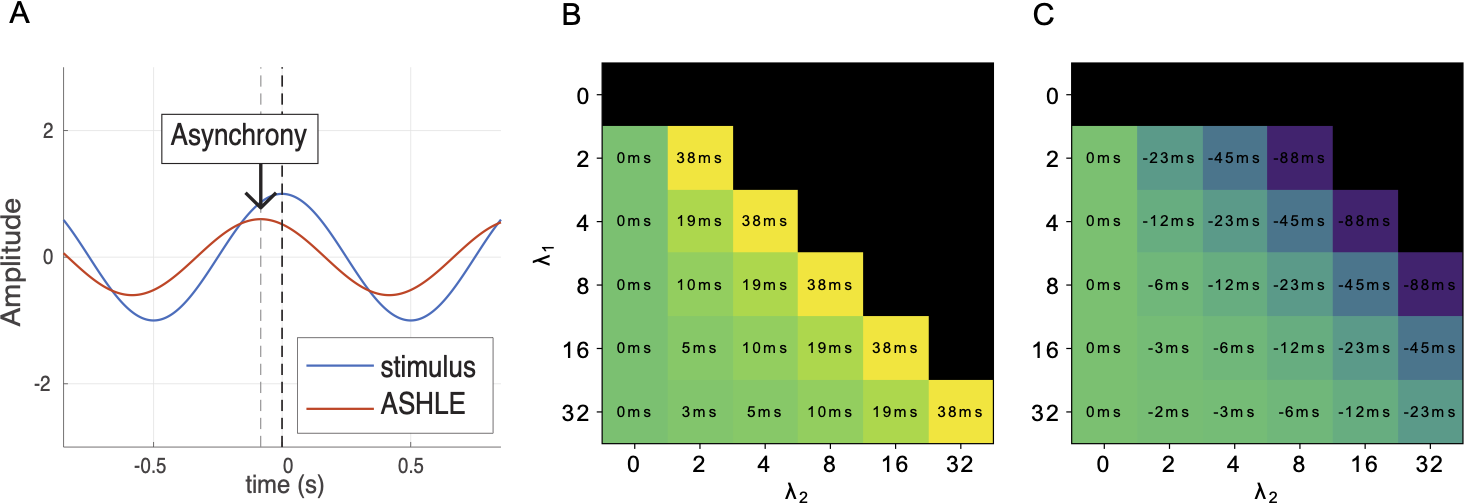
\includegraphics[width=1.0\textwidth]{figures/fig3_6.png}
    \caption[The asynchrony between ASHLE and a sinusoid 45\% faster or slower than ASHLE's ONT as a function of tempo learning and elasticity parameters]{\textbf{The asynchrony between ASHLE and a sinusoid 45\% faster or slower than ASHLE's ONT as a function of tempo learning and elasticity parameters.} (A) Illustration of the asynchrony between ASHLE's $z_m$ and the external sinusoidal stimulus, and how it is measured. (B) The asynchrony in milliseconds between ASHLE and a sinusoidal stimulus 45\% faster than ASHLE's ONT, and its change as a function of $\lambda_1$ and $\lambda_2$, which are ASHLE's parameters for tempo learning and elasticity, respectively. (C) The asynchrony in milliseconds between ASHLE and a sinusoidal stimulus 45\% slower than ASHLE's ONT, and its change as a function of $\lambda_1$ and $\lambda_2$ values. Black cells indicate $\lambda_1$ and $\lambda_2$ value pairs for simulations where ASHLE and the sinusoidal stimulus could not synchronize.}
    \label{f3_6}
\end{figure}

Our second analysis focused on narrowing down our search for parameter values for $\lambda_1$ and $\lambda_2$ that result in asynchronies in the range observed in human data. In the experiment by Scheurich and colleagues \cite{scheurich2018tapping}, musicians synchronized with a stimulus that is 15\% or 30\% faster or slower than their SMT to measure the mean adjusted asynchrony (which is equal to the MA observed during music performance with a metronome tempo different from the musician SMT, minus the MA measured during music performance with an metronome matching the musician SMT). Musicians showed mean adjusted asynchrony values in the range of -10ms and 10ms (see Fig.{} \ref{f3_2}A). In this analysis we ran simulations where ASHLE was stimulated by a different stimulus tempo to measure the MA between an ASHLE model with a ONT $f_0 = 2.5$ (same as our first analysis) and a sinusoidal stimulus $x(t) = \exp(i2\pi f_s t)$ with six potential $f_s$ values: 45\% faster ($f_s = \frac{1000\text{ms}}{0.55 \times 400\text{ms}}$), 30\% faster ($f_s = \frac{1000\text{ms}}{0.70 \times 400\text{ms}}$), 15\% faster ($f_s = \frac{1000\text{ms}}{0.85 \times 400\text{ms}}$), 15\% slower ($f_s = \frac{1000\text{ms}}{1.15 \times 400\text{ms}}$), 30\% slower ($f_s = \frac{1000\text{ms}}{1.30 \times 400\text{ms}}$), and 45\% slower ($f_s = \frac{1000\text{ms}}{1.45 \times 400\text{ms}}$) than the ONT. In our first parameter analysis, we noticed that values for $\lambda_1$ between 3 and 5, and $\lambda_2$ between 1 and 3 could result in MA values in the range of the mean adjusted asynchrony observed in humans (Fig.{} \ref{f3_6}B and \ref{f3_6}C). In this analysis we refine our search for $\lambda_1$ and $\lambda_2$ in this range of values. We ran simulations in a similar fashion to our first analysis. ASHLE and the sinusoidal stimulus interacted for 50 seconds. ASHLE had initial conditions $z_e(0)=z_m(0)== 0.001 + i0$ and $f_e(0)=f_m(0)=f_0$. In Eq \eqref{eq:3.6} the parameter $\gamma=0$ because we want this term to be negligible when a stimulus is present. For each simulation, we found the location (in milliseconds) of the local maxima in the real part of the oscillatory activity of ASHLE's $z_m$ and $x(t)$. Then, we subtracted the location of the peaks of $x(t)$ from the location of the peaks of $z_m$ and averaged the result to obtain the MA in milliseconds. If $z_m$ and $x(t)$ showed a different number of peaks, that indicated that phase-locked synchronization did not occur between the two. Fig.{} \ref{f3_7} shows the result of this analysis. Each subplot shows the asynchrony between $z_m$ and $x(t)$ for a different stimulus tempo and a pair of parameter values of $\lambda_1$ and $\lambda_2$. This analysis revealed that the values of $\lambda_1 = 4$ and $\lambda_2 = 2$ result in the range of MA values observed in humans. This analysis, however, focused on finding parameter values so that ASHLE can capture paced musician synchronization. We also want ASHLE to be able to capture musician behavior during unpaced musical performance, so carried out a third parameter analysis to understand ASHLE's behavior in the absence of a stimulus.

\begin{figure}
    \centering
    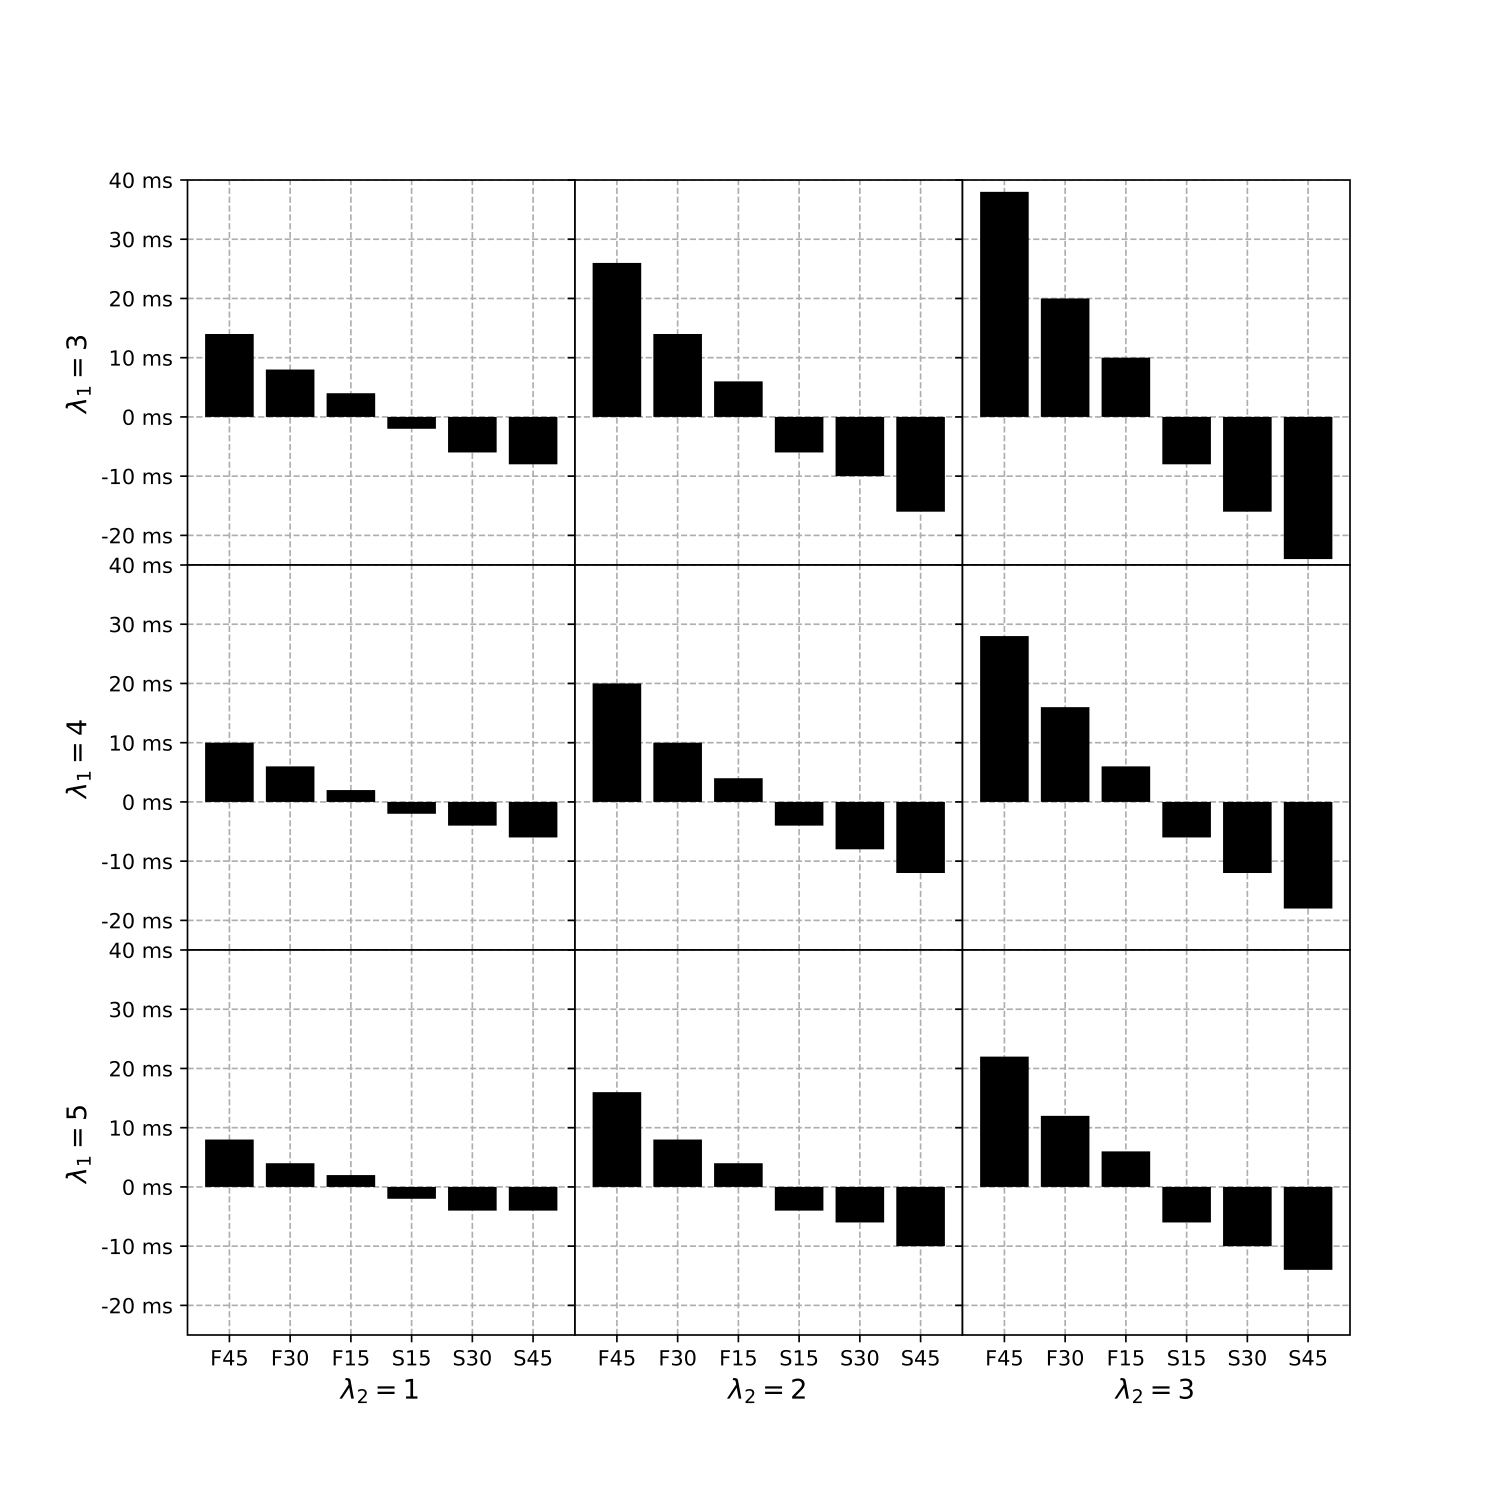
\includegraphics[width=1.0\textwidth]{figures/fig3_7.png}
    \caption[The asynchrony between ASHLE and a sinusoid faster or slower than ASHLE's ONT as a function of a narrower range of values for the tempo learning and elasticity parameters]{\textbf{The asynchrony between ASHLE and a sinusoid faster or slower than ASHLE's ONT as a function of a narrower range of values for the tempo learning and elasticity parameters.} Each cell shows the MA between ASHLE and a sinusoidal stimulus that is 45\% faster, 30\% faster, 15\% faster, 15\% slower, 30\% slower, and 45\% slower than ASHLE's ONT, for a pair of values for $\lambda_1$ and $\lambda_2$, which are ASHLE parameters for tempo learning and elasticity, respectively. The pair of $\lambda_1=4$ and $\lambda_2=2$ yield MA values similar to the ones that Scheurich and colleagues \cite{scheurich2018tapping} observed in musicians synchronizing with a metronome 45\% faster, 30\% faster, 15\% faster, 15\% slower, 30\% slower, and 45\% slower than the musician's SMT.}
    \label{f3_7}
\end{figure}

In our third parameter analysis we observed how, in the absence of an external stimulus (i.e., $F = 0$), the parameter $\gamma$ affects the return of ASHLE to $f_0$ when the initial instantaneous values of $f_e$ and $f_m$ are different than $f_0$. This situation would occur in simulations where ASHLE learned a tempo different than its $f_0$ from a stimulus and then stimulus stops, or if $f_e(0)$ and $f_m(0)$ are set to initial conditions different than $f_0$ in the absence of a stimulus. In the experiment by Zamm and colleagues \cite{zamm2018musicians}, musicians spontaneously started performing at a tempo faster or slower than their SMTs. A linear regression of the consecutive IOI lengths between tempo beats resulted in a slope that revealed that musicians progressively shrank or widened consecutive IOIs, indicating a tendency to return to their SPR. In this experiment musicians showed mean adjusted slope values in the range of -0.2 and 0.1 (see Fig.{} \ref{f3_3}). To simulate this behavior, we need to identify the value of $\gamma$ that will result in similar slope values between consecutive IOIs. In this analysis ASHLE has an ONT $f_0= 2.5$ (same as in the previous two analyses) and in different simulations the initial conditions for $f_e(0)$ and $f_m(0)$ were set to one of four different values: 45\% faster ($f_s = \frac{1000\text{ms}}{0.55 \times 400\text{ms}}$), 30\% faster ($f_s = \frac{1000\text{ms}}{0.70 \times 400\text{ms}}$), 15\% faster ($f_s = \frac{1000\text{ms}}{0.85 \times 400\text{ms}}$), 15\% slower ($f_s = \frac{1000\text{ms}}{1.15 \times 400\text{ms}}$), 30\% slower ($f_s = \frac{1000\text{ms}}{1.30 \times 400\text{ms}}$), and 45\% slower ($f_s = \frac{1000\text{ms}}{1.45 \times 400\text{ms}}$) than the ONT. In all simulations there was no external stimulus (i.e., $F = 0$). We analyzed the behavior of ASHLE for $\gamma$ values of $0.01$, $0.02$, $0.04$, $0.08$. In each simulation, ASHLE oscillated for 50 seconds with initial conditions $z_e(0)=z_m(0)=0.001 + i0$. After each simulation, we found the location (in milliseconds) of the local maxima in the real-part of the oscillatory activity of $z_m$. Then we found the difference between consecutive local maxima to obtain a sequence of IOIs. Finally, we calculated the linear regression between consecutive IOIs to obtain the resulting slope. Fig.{} \ref{f3_8} shows the results of this analysis. Each subplot shows the slopes obtained with different $\gamma$ values and different initial conditions for $f_e(0)$ and $f_m(0)$. This analysis revealed that a value around $\gamma= 0.02$ will match the range of slope values observed in human data.

\begin{figure}
    \centering
    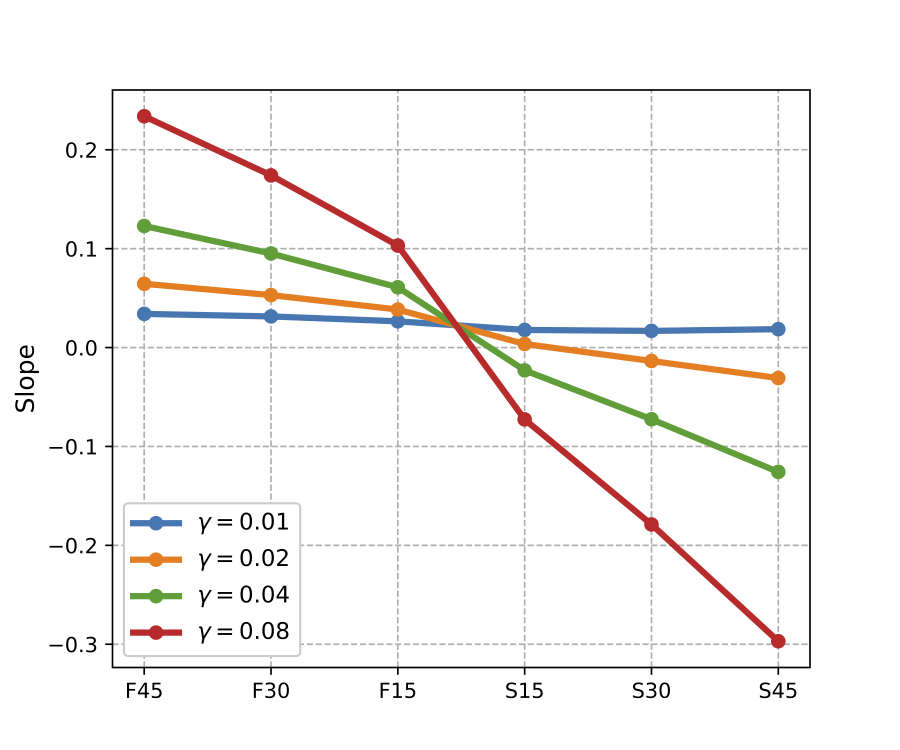
\includegraphics[width=1.0\textwidth]{figures/fig3_8.png}
    \caption[ASHLE slope values as a function of $\gamma$ and initial instantaneous tempo in the absence of a stimulus]{\textbf{ASHLE slope values as a function of $\gamma$ and initial instantaneous tempo in the absence of a stimulus.} The effect of the $\gamma$ parameter on the slope values between consecutive period lengths when ASHLE oscillates without a pacing stimulus, starting at an instantaneous tempo that is 45\% faster ($f_s = \frac{1000\text{ms}}{0.55 \times 400\text{ms}}$), 30\% faster ($f_s = \frac{1000\text{ms}}{0.70 \times 400\text{ms}}$), 15\% faster ($f_s = \frac{1000\text{ms}}{0.85 \times 400\text{ms}}$), 15\% slower ($f_s = \frac{1000\text{ms}}{1.15 \times 400\text{ms}}$), 30\% slower ($f_s = \frac{1000\text{ms}}{1.30 \times 400\text{ms}}$), and 45\% slower ($f_s = \frac{1000\text{ms}}{1.45 \times 400\text{ms}}$) than the ONT.}
    \label{f3_8}
\end{figure}

\subsection{Experiment 1: Solo music performance with a metronome tempo \\ different than the SMT}

\subsubsection{Behavioral data for simulation}

In the task by Scheurich and colleagues \cite{scheurich2018tapping}, 20 musicians individually performed a simple melody while synchronizing with a metronome in four experimental tempo conditions: 30\% faster, 15\% faster, 15\% slower, and 30\% slower than their SMT. For each metronome rate, participants performed the melody ("Mary had a little lamb") four consecutive times (32 beats per repetition, 128 beats total). Experimenters measured the mean adjusted asynchrony between the participant tempo and the experimental metronome rate during the middle two melody repetitions (64 beats total). The mean adjusted asynchrony is the MA observed when the musician performs with a metronome tempo different than the musician's SMT, minus the MA observed when the musician performs with a metronome that matches the SMT. Scheurich and colleagues \cite{scheurich2018tapping} used the mean adjusted asynchrony instead of the MA to assume in their analysis that no MA exists between the musician and the metronome when the metronome tempo matches the musician's SMT. Fig.{} \ref{f3_2}A shows the behavioral data with the mean adjusted asynchrony (average and standard error) observed across all 20 musicians for each experimental metronome tempo condition. Their results showed that the mean adjusted asynchrony had a tendency to be positive when synchronizing with a metronome faster than the SMT (musician actions lagging the metronome), and negative when synchronizing with a metronome slower than the SMT (musicians actions anticipating the metronome). Additionally, the mean adjusted asynchrony grew as a function of the difference between musician SMT and experimental metronome tempo.

\subsubsection{Setup, procedures and measurements} 

To obtain the musicians SMTs, we overlaid a grid over Figure 4 from the paper by Scheurich and colleagues \cite{scheurich2018tapping}, which showed each musician's measured SMT. Using this grid over the original figure allowed us to precisely digitize each musician's SMT from the original publication. Using the musician SMT values, we simulated 20 different ASHLE models, all with the same parameter values (see model optimization below) except for the ONT, which matched the SMT of a different musician. ASHLE does not generate pitch, so it only simulates the beats of the melody that musicians performed, not the melody or harmony content. This is not a problem, however, since Scheurich and colleagues only analyzed each musician's beat performance. In all simulations, initial conditions were $z_e(0)=z_m(0)= 0.001 + i0$ (indicating that ASHLE's two oscillators start with zero phase), $f_e(0)=f_m(0)=f_0$ (where $f_0$ is ASHLE's ONT equivalent in hertz: $f_0=\frac{1000 \text{ms}}{\text{ONTms}}$. Following the procedure in the musician experiment, each ASHLE synchronized during 128 cycles with a pacing complex-valued sinusoidal stimulus $x(t)=\exp(i2\pi f_s t)$ where $f_s$ was either 30\% faster ($f_s=\frac{1000 \text{ms}}{0.7 \times \text{ONTms}}$), 15\% faster ($f_s=\frac{1000 \text{ms}}{0.85 \times \text{ONTms}}$), 15\% slower ($f_s=\frac{1000 \text{ms}}{1.15 \times \text{ONTms}}$), or 30\% slower ($f_s=\frac{1000 \text{ms}}{1.3 \times \text{ONTms}}$) than the ONT. We also simulated how ASHLE would synchronize with a metronome tempo 45\% faster ($f_s=\frac{1000 \text{ms}}{0.55 \times \text{ONTms}}$) or 45\% slower ($f_s=\frac{1000 \text{ms}}{1.45 \times \text{ONTms}}$) in order to make predictions about how musicians would perform in those additional experimental conditions. After each simulation, we identified the location (in milliseconds) of local maxima in the real part of ASHLE's effector $z_m$ and the sinusoidal stimulus. Then, in each simulation we identified the middle 64 peaks for ASHLE and the stimulus and subtracted the location of stimulus peaks from ASHLE peaks to obtain the asynchrony. Averaging these asynchronies in each simulation resulted in the MA for a specific simulation. To obtain the mean adjusted asynchrony that Scheurich and colleagues used in their analysis, from each MA obtained in the experimental conditions, we subtracted the MA observed when ASHLE synchronized with a sinusoid with a tempo that matched ASHLE's ONT ($f_s=f_0$). We averaged the mean adjusted asynchronies observed across the 20 ASHLE models that me simulated (only different by their ONT value) for each stimulus rate (15\%, 30\%, or 45\% faster than ASHLE's ONT) to obtain the plot in Fig.{} \ref{f3_2}B. We also simulated how different ASHLE models with specific ONT values linearly spaced between 350ms and 650ms would carry out this task when synchronizing with a stimulus tempo that is 45\% faster ($f_s=\frac{1000 \text{ms}}{0.55 \times \text{ONTms}}$), 30\% faster ($f_s=\frac{1000 \text{ms}}{0.7 \times \text{ONTms}}$), 15\% faster ($f_s=\frac{1000 \text{ms}}{0.85 \times \text{ONTms}}$), 15\% slower ($f_s=\frac{1000 \text{ms}}{1.15 \times \text{ONTms}}$), 30\% slower ($f_s=\frac{1000 \text{ms}}{1.3 \times \text{ONTms}}$), or 45\% slower ($f_s=\frac{1000 \text{ms}}{1.45 \times \text{ONTms}}$) than the ONT. Fig.{} \ref{f3_2}C shows the results of these simulations, which are predictions of musician data that could be collected to test the accuracy of predictions made by ASHLE.

\subsubsection{Model optimization} 

Our goal was to use ASHLE to simulate the results in the musician data by Scheurich and colleagues \cite{scheurich2018tapping}. In all our simulations in this experiment, some ASHLE parameters were always the same: $\alpha=1$, $\beta=-1$, and $\gamma=0.02$ (see model optimization for experiment 2 to understand how we came to this exact value for $\gamma$). The other two parameters that were always the same across simulations were $\lambda_1=4$ and $\lambda_2=2$, which we found in our parameter analysis to result in a good approximation of the musician data results by Scheurich and colleagues \cite{scheurich2018tapping}. When we carried out the simulations in this experiment, we confirmed that the values of $\lambda_1=4$ and $\lambda_2=2$ resulted in a good fit between our simulations and the musician data by Scheurich et al. \cite{scheurich2018tapping}.

\subsection{Experiment 2: Unpaced solo music performance with a \\ starting tempo different than the SMT}

\subsubsection{Behavioral data for simulation}

In the task by Zamm et al. \cite{zamm2018musicians}, 24 musicians individually performed a simple melody without listening to a metronome. In one control condition they performed the melody at their SMT, and in four other experimental conditions they performed starting at four other spontaneous tempi: fast and slow with respect to SMT, and even faster and slower with respect to the SMT. For each spontaneous initial tempo, musicians performed the melody ("Frere Jaques") four consecutive times (32 beats per repetition, 128 beats total). For each tempo, experimenters measured the IOI between melody beats across each musician's entire performance and carried out a linear regression to obtain a slope, which indicates the rate of change across IOIs over the entire performance. Fig.{} \ref{f3_3}A shows the behavioral data with the average slope across participants in each initial tempo condition. Results showed that the slope had a tendency to be positive when performances started a spontaneous tempo faster than the SMT (IOIs becoming longer as the performances progressed), and negative when performances started at a spontaneous tempo slower than the SMT (IOIs becoming shorter as the performance progressed).

\subsubsection{Setup, procedures and measurements}

To obtain the musicians' SMT, we overlaid a grid over Figure 1 from the paper by Zamm and colleagues \cite{zamm2018musicians}, which showed each musician's measured SMT. We also overlaid a grid over Figure 2 (right top panel) from the same paper by Zamm and colleagues to obtain each musician's initial rates of performance that were fast, slow, faster, and slower with respect to their SMT. Using these grids over original musician data figures allowed us to precisely recover each musician's rates of performances reported in the original study. Because our model does not generate pitch, it only simulates the beats of the melody that musicians performed, not the individual notes. Using the musicians' SMT and initial performance tempo values, we simulated 23 different ASHLE models, each oscillating with 5 different initial conditions for $f_e(0)=f_m(0)$ (matching the SMT, fast or slow compared to the SMT, and faster and slower than the SMT) (115 total simulations). We did not simulate the participant with the SMT of 665ms because its fast spontaneous tempo was signficantly faster than the rest of the particpant fast tempi, and ASHLE was not able to show stable activity as a result of this tempo difference. In all simulations in this experiment there was no stimulus ($F = 0$). All simulations shared the same parameter values (see model optimization below) except for the ONT (which matched the SMT of a different musician) and each simulation started with the ASHLE model having different initial conditions for $f_e(0)=f_m(0)$. After each simulation, we identified the location (in milliseconds) of local maxima in the real part of ASHLE's effector $z_m$. Then, we measured the difference between consecutive peaks to analyze how IOIs change over the course of a simulation. For each simulation we carried out a linear regression over the IOIs to obtain a slope value. Consistent with the methods in the human experiment to obtain the adjusted slope, the slope of each simulation in the control condition where $f_e(0)=f_m(0)=f_0$ was subtracted from the slope obtained in the experimental conditions ($f_e(0)=f_m(0)\neq f_0$). We averaged adjusted slopes across ASHLE models for each experimental initial tempo condition to obtain the plot in Fig.{} \ref{f3_3}B. We also simulated how different ASHLE models with specific ONT values linearly spaced between 350ms and 650ms would carry out this task when the initial conditions for $f_e(0)=f_m(0)$ were consistently 45\% faster ($f_e(0)=f_m(0)=\frac{1000\text{ms}}{0.55 \times \text{ONTms}}$), 30\% faster ($f_e(0)=f_m(0)=\frac{1000\text{ms}}{0.70 \times \text{ONTms}}$), 15\% faster ($f_e(0)=f_m(0)=\frac{1000\text{ms}}{0.85 \times \text{ONTms}}$), 15\% slower ($f_e(0)=f_m(0)=\frac{1000\text{ms}}{1.15 \times \text{ONTms}}$), 30\% slower ($f_e(0)=f_m(0)=\frac{1000\text{ms}}{1.3 \times \text{ONTms}}$), and 45\% slower ($f_e(0)=f_m(0)=\frac{1000\text{ms}}{1.45 \times \text{ONTms}}$) than the ONT. Fig.{} \ref{f3_3}C shows the results of these simulations, which are predictions of musician data that could be collected to test the accuracy of predictions made by ASHLE.

\subsubsection{Model optimization}

Our goal was to use the ASHLE model to simulate the results in the musician data by Zamm and colleagues \cite{zamm2018musicians}. With the exception of $F = 0$	(due to the lack of stimulus), in this second experiment we used the same parameters used in experiment 1. We wanted to use the same parameter values in order to validate our model's behavior across two different sets of behavioral results. Hence, in all simulations in this second experiment $\alpha = 1$, $\beta = −1$, and $\gamma = 	0.02$. Similarly, initial conditions for Eqs \eqref{eq:3.5} and \eqref{eq:3.7} were the same between experiment 1 and experiment 2. The only set of parameters that varied between simulations were the initial conditions for $f_e(0)=f_m(0)$ and the oscillators ONT ($f_0$).

\subsection{Experiment 3: Duet musical performance between musicians \\ with matching or mismatching SMTs}

\subsubsection{Behavioral data for simulation}

In another experiment, Zamm and colleagues \cite{zamm2016endogenous} measured the SMT of 40 musicians and formed duets of musicians in two experimental groups: duets with matching SMTs (<10ms IOI difference), and duets with mismatching SMTs (>110ms IOI difference). There were 10 unique musician duets in each experimental group. Musician pairs were instructed to perform a simple unfamiliar melody together (16 beats in length), repeating the melody four consecutive times (64 beats total). When pairs of musicians performed the task, they first heard four metronome beats (400ms IOI) that established the common tempo. Experimenters measured the absolute asynchrony between each pair of synchronizing musicians throughout the entire performance. Because the same melody was repeated four times, they obtained a mean absolute asynchrony for each of the melody repetitions. Fig.{} \ref{f3_4}A shows the behavioral data reported by Zamm and colleagues (2016) with the average mean absolute asynchrony across musicians for each melody repetition and for each experimental group. Results showed that the mean absolute asynchrony between duets of musicians was larger when their SMTs did not match compared to when they matched.

\subsubsection{Setup, procedures and measurements}

To obtain the musicians' SMTs, we overlaid a grid over Figure 1 from the paper by Zamm and colleagues \cite{zamm2016endogenous}, which showed each musician's measured SMT. Using the grid over the original figure allowed us to precisely recover each musician's SMT as reported in the original study. Because our model does not generate pitch, it only simulates the beats of the melody that musicians performed, not the individual notes. Using the musicians' SMT values, we simulated 20 pairs of ASHLE models (10 pairs with similar SCRs and 10 pairs with dissimilar SCRs) synchronizing during 64 cycles. All simulations shared the same parameter values and initial conditions used in experiment 1, except for $F$ (see model optimization in the next paragraph) and the ONT, which matched the SMT of a musician in the data by Zamm and colleagues \cite{zamm2016endogenous}. At the beginning of the simulation, two ASHLE models were stimulated by a complex-valued sinusoid $x(t)=\exp(i2\pi	f_s t)$ with an IOI of 400ms ($f_s = 2.5$). After these four cycles of sinusoidal stimulation, the sinusoidal stimulus stopped and the two ASHLE models stimulated each other with their respective $z_m$. That is, in each duet simulation, after four cycles of sinusoidal stimulation, the input to the ASHLE No.1 was $F_z z_{m_2}$ and the input to ASHLE No.2 was $F_z z_{m_1}$, where $F_z$ is the forcing strength between ASHLE models. After each simulation, we identified the location (in milliseconds) of local maxima in the real part of each ASHLE's effector $z_m$. Then, we measured the absolute asynchrony between the two synchronizing ASHLE model's $z_m$, obtaining 64 absolute asynchronies for each simulation. We divided these 64 absolute asynchronies in four subsections of equal parts (16 absolute asynchronies per section) to simulate the four melody repetitions that pairs of musicians carried out in the experiment by Zamm et al. \cite{zamm2016endogenous}, and we averaged the mean absolute asynchrony in each of these four subsections. We averaged the mean absolute asynchronies across pairs of ASHLE models for each melody repetition to obtain the plot in Fig.{} \ref{f3_4}B. We also simulated how different ASHLE models with specific ONT values linearly spaced between 350ms and 650ms would carry out this task when synchronizing for 16 cycles with another ASHLE model with an ONT difference of -220ms, -110ms, -10ms, 10ms, 110ms, and 220ms. Fig.{} \ref{f3_4}C shows the results of these simulations, which are predictions of data that could be collected to test the accuracy of predictions made by ASHLE.

\subsubsection{Model optimization}

Our goal was to use the ASHLE model to simulate the results in the study by Zamm and colleagues \cite{zamm2016endogenous}. With the exception of the stimulus forcing $F$ and $F_z$, in this second experiment we used the same parameters used in experiment 1 and 2. Hence, in all simulations in this experiment $\alpha = 1$, $\beta = −1$, and $\gamma = 0.02$. Similarly, initial conditions for Eqs \eqref{eq:3.5} and \eqref{eq:3.7} were always $z_e(0)=z_m(0)=0.001 + i0$ and $f_e(0)=f_m(0)=f_0$ (matching the SMT by each musician in the study by Zamm and colleagues \cite{zamm2016endogenous}). In contrast with the previous two experiments, there were two kinds of stimulation in this third experiment. During the first four cycles of each simulation, similar to experiment 1, ASHLE was simulated by a sinusoid $x(t)=\exp(i2\pi f_s t)$ with a force $F = 1$ and $f_s=2.5$. However, during the next 64 cycles, two ASHLE models synchronized with each other, so the input to the first ASHLE model is the second ASHLE model's effector $F_z z_{m_2}$ and the input to the second ASHLE model was the first ASHLE model's effector $F_z z_{m_1}$. We found that using an $F_z = 1$ resulted in a lack of phase-locked synchronization between the two ASHLE, suggesting that $F_z = 1$ is too large and causes unstable dynamics between the two interacting ASHLE models. To improve stability, we reduced the value of $F_z$ until we observed stable synchronization between all pairs of ASHLE models that we want to simulate. We found that $F_z = 0.01$ resulted in stable synchronization, and mean absolute asynchronies matching the range of values in the behavioral data. However, we also noted that the mean absolute asynchrony was considerably smaller between pairs of ASHLE models with similar ONTs compared to the human results for musician duets with matching SMTs. We believe that this difference was due to the lack of noise in our model. To improve our simulation results, in each simulation we added gaussian noise to ASHLE's effector $z_m$ turning Eq \eqref{eq:3.7} into:

\begin{equation}
\frac{1}{f_m}\dot{z}_m = z_m \left( \alpha + i2\pi + \beta|z_m|^2 \right) + \exp(i \angle z_e) + \mathcal{N}(\mu, \sigma^2) \label{eq:3.9}
\end{equation}

where $\mu=0$ is the mean and $\sigma=10$ is the standard deviation of a normal distribution. Fig.{} \ref{f3_4}B shows the results obtained after we added the noise, which better approximate the behavioral data.

\chapter{Motivations to combine delayed feedback and elastic Hebbian frequency learning}
\chaptermark{Combining delayed feedback \& elastic hebbian learning}

In this chapter we describe future work that can be done using the SAPPA and ASHLE models described in the previous two chapters. These models capture different types of periodic sensorimotor synchronization. While both share the oscillatory dynamics of the equation originally described by Large and colleagues \cite{large2010canonical}, their biopysical mechanisms are very different. The SAPPA model involves delayed feedback to capture the anticipation tendencies observed in humans, while the ASHLE model involves Hebbian learning and elasticity to capture adaptive synchronization affected by the spontaneous motor tempo (SMT). On their own, these models have limitations but a more robust model could be developed by combining all their dynamic mechanisms.

A major limitation of the SAPPA model is its complete lack of variability. In our experiments with the SAPPA model, we identified two different delayed feedback amplitudes able to simulate the negative mean asynchrony (NMA) that Repp and Doggett \cite{repp2007tapping} observed in groups of musicians and a non-musicians. In our simulations, a single SAPPA model captured all musician results, and another SAPPA model simulated all non-musician results. The only difference between these two models was the amplitude of the delayed feedback term. This makes the SAPPA model parsimonious and able capture the average NMA observed in a group consisting of musicians and another group consisting of non-musician. However, the SAPPA model cannot explain the NMA differences between individuals in a group. Moreover, the frequency term in the SAPPA model is fixed and has to be manually tuned to match a periodic stimulus tempo and simulate the NMA. 

In contrast to SAPPA, the ASHLE model does not suffer from a complete lack of variability in its behavior. ASHLE's frequency term is dynamically learned from a stimulus. Additionally, ASHLE can simulate the SMT at the individual level (not the group level). Moreover, our simulations show that noise can be added to add variability to ASHLE's instantaneous activity. However, the ASHLE model lacks the delayed feedback term present in the SAPPA model and it must be studied whether the ASHLE model can capture the NMA to the same extent that the SAPPA model does. These two models, SAPPA and ASHLE, represent hypotheses about the biophysical mechanisms of NMA and tempo adaptation.

The human data simulated by SAPPA and ASHLE is different. While SAPPA simulated the actual asynchronies that humans showed \cite{roman2019delayed}, the data simulated by ASHLE consisted of adjusted asynchronies \cite{scheurich2018tapping}, adjusted slopes \cite{zamm2018musicians}, and absolute asynchronies \cite{zamm2016endogenous}. Additionally, in the behavioral data simulated by SAPPA the individual's SMT was not measured or accounted for. Moreover, in the behavioral data simulated by ASHLE, the mean asynchrony and the spontaneous slope were removed to obtain the adjusted asynchrony and the adjusted slope measurements, respectively. These differences between SAPPA and ASHLE data simulations are critical, and should be accounted for in future experimental and theoretical research. 

Given the differences between the SAPPA and ASHLE models, a logical next step would be to combine them. If we assume that the ASHLE model optimally captures the variability of human synchronization, the next step could be as simple as adding the SAPPA model's delayed feedback term to the ASHLE model. Doing this would simply add ``strong anticipation" (see chapter 2) to the ASHLE model. The resulting model could be named Strong Anticipation in Adaptive Synchronization with Hebbian Learning and Elasticity (SAASHLE). 

In SAASHLE, the elasticity and strong anticipation mechanisms would be redundant when simulating human synchronization with a stimulus slower than an individual's SMT. For the specific case of musicians, this redundancy would be negligible because the delayed feedback amplitude originally found for SAPPA is relatively small. However, in the case of non-musicians, this redundancy would be observed in the model's activity. This is not necessarily a bad thing, because such redundancy exists in the dynamical mechanisms of adaptive synchronization and anticipation observed in non-musicians. Behavioral data supports this observation. In the original publication by Scheurich and colleagues \cite{scheurich2018tapping}, their Figure 5 shows the asynchrony observed across musicians (top) and non musicians (bottom) that performed a melody with a metronome 15\% and 30\% faster slower than the individual's SMT. While the musician data shows a similar asynchrony for the faster and slower conditions, the non-musicians show larger negative asynchronies for the slower rate conditions than the faster rate conditions \cite{scheurich2018tapping}. ASHLE on its own would not be able to capture this difference between musicians and non-musicians. However, adding SAPPA's strong anticipation to ASHLE will capture the dynamical mechanisms of this difference observed between musicians and non-musicians. SAASHLE will also be able to capture the variability observed in all human data described in Chapter 2 that SAPPA could not explain. In general, by understanding the dynamics of PAC behavior, we can constrain models like ASHLE, SAPPA, or SAASHLE, and we can motivate future experiments. 

All these considerations indicate that future research should aim at developing the SAASHLE model that we have described in this chapter. SAASHLE parameters should be optimized to capture the musician and non-musican data collected by Scheurich and colleagues \cite{scheurich2018tapping}. Subsequently, SAASHLE must be validated by its ability to capture the human data in all other simulations described in chapters 2 and 3. 

SAASHLE will be a powerful model able to capture adaptive synchronization via the dynamical mechanisms of delayed axonal delays (simulated with strong anticipation \cite{stepp2010strong}), neural population entrainment to auditory stimulus (simulated with Hebbian learning \cite{righetti2006dynamic}), and the motor constraints that give rise to the SMT (simulated with elasticity \cite{lambert2016adaptive}). SAASHLE will also capture variability within and between subjects, as well as the effects of musician training via the delayed feedback amplitude difference between musician and non-musician models. 


\chapter{Next-generation gradient frequency neural networks}
\chaptermark{Next-Generation GrFNNs}

\section{Abstract}
The neural oscillators in a gradient frequency neural network (GrFNN) are similar to the neurons found in deep neural networks, but each GrFNN unit has its own intrinsic temporal dynamics. Because of their rich set of parameters and dynamics, GrFNNs can carry out pattern recognition with or without memory, signal filtering, and Hebbian learning. To optimize GrFNNs parameters, one can carry out a steady-state analysis with a desired amplitude, frequency and phase. This is mathematically straightforward when the GrFNN stimulus is simple, like a pure tone or a song with a constant tempo frequency. However, finding GrFNN parameters is more challenging when the stimulus is noisy, like recordings of speech in real-world environments. We propose that the next generation of GrFNNs should be optimized via gradient descent. We present the first implementation of GrFNNs with tensorflow 2, allowing for automatic differentiation of GrFNN parameters and gradient descent optimization. We carry out two experiments with our implementation. The first one demonstrates that gradient descent can be used to find GrFNN parameters for previously known dynamical states, like limit cycles. The second experiment shows how GrFNN parameters can be optimized with a data-driven approach, similar to deep neural networks. Besides gradient descent optimization, this new implementation allows for future research that integrates GrFNNs as building blocks of deep learning algorithms and other machine learning methods.

\section{Introduction}

The work presented in the preceding chapters uses the canonical oscillator introduced by Large and colleagues \cite{large2010canonical} (see the methods section in chapters 2 and 3 for a detailed description of this equation).  

\begin{equation}
\frac{1}{f}\dot{z} = z\bigg(\alpha + i2\pi + \beta_1|z|^2 + \frac{\epsilon\beta_2|z|^4}{1-\epsilon|z|^2}\bigg) + x(t) \label{eq:5.1}
\end{equation}

The SAPPA (described in chapter 2) and ASHLE (described in chapter 3) models only use one such oscillator each, but in the original publication by Large and colleagues, multiple oscillators were interconnected to form a network where each oscillator had a different natural frequency \cite{large2010canonical}. A network of these oscillators results in a model called gradient frequency neural network (GrFNN). A GrFNN shows complex behavior and dynamics that emerge from the interactions between oscillators. The oscillators in a GrFNN are derived from a biological model of neural oscillation observed in the brain, and since their original publication, scientific investigations have shown that GrFNNs can explain the synchronization dynamics observed in real human brain data \cite{tal2017neural}. Moreover, GrFNNs have also been used to simulate the tonotopy and mechanics of the cochlea, including its nonlinearities \cite{lerud2019canonical}.

Besides modeling behavioral and neural data, GrFNNs have properties for signal processing of time-series signals \cite{kim2015signal}. GrFNNs are a generalization of gammatone filter banks \cite{large2015learning}, they can identify temporal patterns, and can amplify or filter periodic features in a signal \cite{kim2015signal}. Some patterns of activity that oscillators in a GrFNN can show include spontaneous limit-cycle activity, which is equivalent to a complex sinusoid, and double limit-cycle activity, which is a memory state that reflects the period of a stimulus even after the stimulus ceases \cite{kim2015signal}. The double limit-cycle dynamics of GrFNNs are possible due to its higher-order nonlinearities (see Eq \eqref{eq:5.1} \cite{large2010canonical, kim2015signal}). Additionally, the oscillators in a GrFNN network can be connected via Hebbian plasticity to adaptively change their connection weights \cite{lambert2016adaptive, kim2017dynamical}. 

GrFNNs are not to be confused with the popular kind of neural networks currently used in deep learning algorithms. There exist some similarities but also differences between the computations in a GrFNN and a deep neural network of the feedforward, recurrent, or convolutional type, to name a few. Both are nonlinear, but for different reasons. In a feedforward neural network, each unit computes the linear combination of weights that multiply input features. Then, each unit's output may be passed through a nonlinear function, like a sigmoid or a rectifier \cite{svozil1997introduction}. Hence, in a feedforward neural network, each unit carries out a linear computation and the unit's output is nonlinearly transformed by a function. The units of convolutional and recurrent neural networks obtain their nonlinear properties in a similar fashion, although recurrent neural networks involve feedback, which can be nonlinear on its own \cite{le2015tutorial2}. Moreover, feedforward and convolutional networks do not process stimuli throughout timesteps and their units are temporally static. This is different in recurrent neural networks, where each unit processes information from the present and the past \cite{le2015tutorial2}. In contrast, the units of GrFNNs have intrinsic nonlinear and temporal dynamics. Each oscillator, or unit, computes the rate of change of its own activity, which depends on a nonlinear transformation of the oscillator's current state (see Eq \eqref{eq:5.1}) \cite{large2010canonical}. 

The optimization of patterns in a GrFNN and a neural network is also different. The parameters in a feedforward neural network, for example, can be optimized via gradient descent. The output is compared against a ground truth via an objective function (like mean squared error, for example), and the objective function's derivative is computed with respect to every parameter to update the feedforward neural network's parameters \cite{le2015tutorial1}. This process to update the model parameters is iterated until the objective function error is maximally reduced. In a GrFNN the parameters $\alpha$, $\beta_1$, $\beta_2$ and $\epsilon$ must be optimized, sometimes independently for each oscillator. However, gradient descent has not been the default approach. Because each oscillator in a GrFNN has a steady state solution, one can set Eq \eqref{eq:5.1} equal to zero to identify the values of $\alpha$, $\beta_1$, $\beta_2$ and $\epsilon$ that result in the desired amplitude and phase of $z$. This analysis reveals solutions with patterns of activity that include Hopf bifurcations, limit-cycles, and double limit-cycles \cite{kim2015signal}. Identifying the desired steady state behavior is possible when the input is tractable (i.e., a pure tone, or a song with a steady beat). However, Eq \eqref{eq:5.1} cannot be solved for a steady state when the input is noisy or more difficult to characterize mathematically (i.e., noisy speech). 

In this investigation we ask the question: can we learn the parameters of a GrFNN via an objective function and gradient descent? To answer this question we implemented the GrFNN toolbox in tensorflow 2 to use automated differentiation via gradient descent with GPU acceleration. This allows for fast computation of ordinary differential equations (ODEs), like GrFNN. Tensorflow has already been proposed as the best tool to simulate large networks of biological neurons with significant gains in computation speed compared to using only python \cite{mohanta2019parallel}. To test our implementation, we carried out two optimization experiments using gradient descent.

In the first experiment we optimize the parameters of a single GrFNN oscillator to show limit-cycle behavior. GrFNN parameters were randomly initialized and optimized via gradient descent using a mean squared error objective that indicated the magnitude of a limit-cycle oscillator.

In the second experiment we optimize the parameters of a GrFNN network to find the best time-frequency mask to clean a noisy speech signal. Convolution of the GrFNN time-frequency mask and a time-frequency transformation of the noisy speech signal resulted in character error rates that beat performance by current deep learning models to clean noisy speech. 

Together, these experiments show that GrFNNs can be optimized via gradient descent, in addition to steady-state analysis. In contrast to steady-state analysis, gradient descent will allow for optimization of GrFNNs when a noisy input makes it hard or even impossible to approximate a desired steady state. Additionally, gradient descent optimization is automatic when using grap-based differentiation methods like Tensorflow. This work also opens the possibility of incorporating GrFNNs into deep learning algorithms. Such hybrid algorithms could improve signal processing via the dynamical properties of GrFNNs and optimization of parameters with gradient descent.

\section{Results}

\subsection{Experiment 1: Gradient descent optimization of a single GrFNN \\ oscillator to show limit-cycle activity} 

In this first experiment we used gradient descent to optimize the parameters of a single GrFNN oscillator. The goal was to obtain parameters that would make the oscillator show limit-cycle activity. GrFNN oscillators showing limit-cycle activity are well understood \cite{kim2015signal}. The previous analysis by Kim and Large reveals that any GrFNN oscillator with $\alpha>0$, $\beta_1<0$, $\beta_2=0$ and $\epsilon=0$ will show a limit-cycle \cite{kim2015signal}. Additionally, if $|\alpha|=|\beta_1|$, the limit-cycle will be unit magnitude. The goal of this experiment is to use gradient descent to find the GrFNN parameters that will result in a unit magnitude limit-cycle in a single oscillator. Fig.{} \ref{f5_1} shows the results. Fig.{} \ref{f5_1}A shows the values of the trainable parameters over the gradient descent iterations. At the beginning, all the values start around zero because the values were drawn from a small normal distribution. As the gradient descent iterations progress, the values of $\alpha$ and $\beta_1$ become positive and negative, respectively. Additionally, because we optimized the limit-cycle to be unit magnitude, the values of $\alpha$ and $\beta_1$ are similar in magnitude. In contrast, the values of $\beta_2$ and $\epsilon$ stay around zero. Fig.{} \ref{f5_1}B and Fig.{} \ref{f5_1}C show the activity of the single GrFNN oscillator at the beginning and the end of the gradient descent process, respectively. Throughout the duration of the simulation shown in Fig.{} \ref{f5_1}B, the oscillator shows the magnitude originally drawn from the normal distribution. In contrast, Fig.{} \ref{f5_1}C shows activity that corresponds to a unit magnitude limit-cycle steady state, resulting from the values of $\alpha$ and $\beta_1$ that were learned through gradient descent in this experiment. 

\begin{figure}
    \centering
    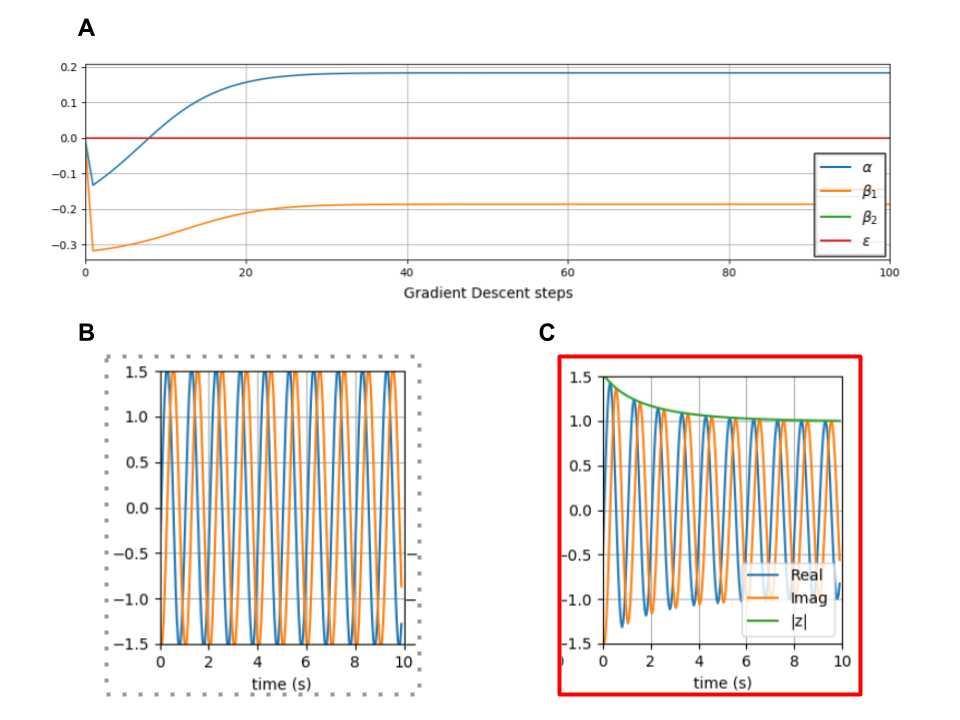
\includegraphics[width=1.0\textwidth]{figures/fig5_1.png}
    \caption[Gradient descent optimization process and resulting activity for a single GrFNN oscillator]{\textbf{Gradient descent optimization process and resulting activity for a single GrFNN oscillator.} (A) The values of the trainable parameters $\alpha$, $\beta_1$, $\beta_2$ and $\epsilon$ that were learned over 100 gradient descent iterations. Because the oscillator learns limit-cycle activity, $\alpha$ and $\beta$ become positive and negative, respectively, while $\beta_2$ and $\epsilon$ remain around their initial values close to zero (the green line corresponding to $\beta_2$ is occluded by the red line that corresponds to $\epsilon$). The oscillator also learns unit magnitude activity, hence why $\alpha$ and $\beta_1$ have similar magnitude. (B) The activity shown by the oscillator in a simulation lasting 10 seconds with the parameter values before gradient descent optimization. The blue and orange lines correspond to the real and imaginary parts of the GrFNN oscillator, respectively. This oscillator with parameter values $\alpha$, $\beta_1$, $\beta_2$ and $\epsilon$ that are very close to zero is equivalent to $\frac{1}{f}\dot{z}=z(i2\pi)$ (compare with Eq \eqref{eq:5.1}), which is an oscillator with sustained magnitude always matching its initial magnitude and frequency dictated by $f$. (C) The activity shown by the oscillator in a simulation lasting 10 seconds with the parameter values learned via gradient descent optimization. The oscillator shows unit magnitude limit-cycle activity.} 
    \label{f5_1}
\end{figure}

This initial experiment shows that it is possible to find the parameters of a single GrFNN oscillator via gradient descent. As long as a well-described steady state is known in advance, iterative gradient descent is a plausible method to find the GrFNN parameters that will result in an oscillator showing such steady state.

\subsection{Experiment 2: Gradient descent optimization of a GrFNN network \\ for speech enhancement.} 

Experiment 1 showed that we can optimize the parameters of a single GrFNN oscillator to show a specific steady state behavior. In this second experiment we tested whether we could learn GrFNN parameters for different oscillators in a network that is used enhance noisy speech. A GrFNN network can process a noisy signal, resulting in oscillators resonating with the signal but not with the noise. In our second experiment, the GrFNN network processed a noisy speech signal to generate a time-frequency mask, which then could be convolved with the original noisy speech to obtain a cleaned version. Fig.{} \ref{f5_2}A shows the processing pipeline where noisy speech is processed by the GrFNN and the noisy speech time-frequency transformation is also calculated. After that step, the time-frequency transformation and the GrFNN output can be combined to obtain a cleaned signal. Fig.{} \ref{f5_2}B shows the results, comparing character error rate (CER) performance of our model against the Speech Enhancement Generative Adversarial Network (SEGAN), which is a state-of-the-art method for speech enhancement \cite{pascual2017segan}. Our model outperforms SEGAN in the CER metric. 

\begin{figure}
    \centering
    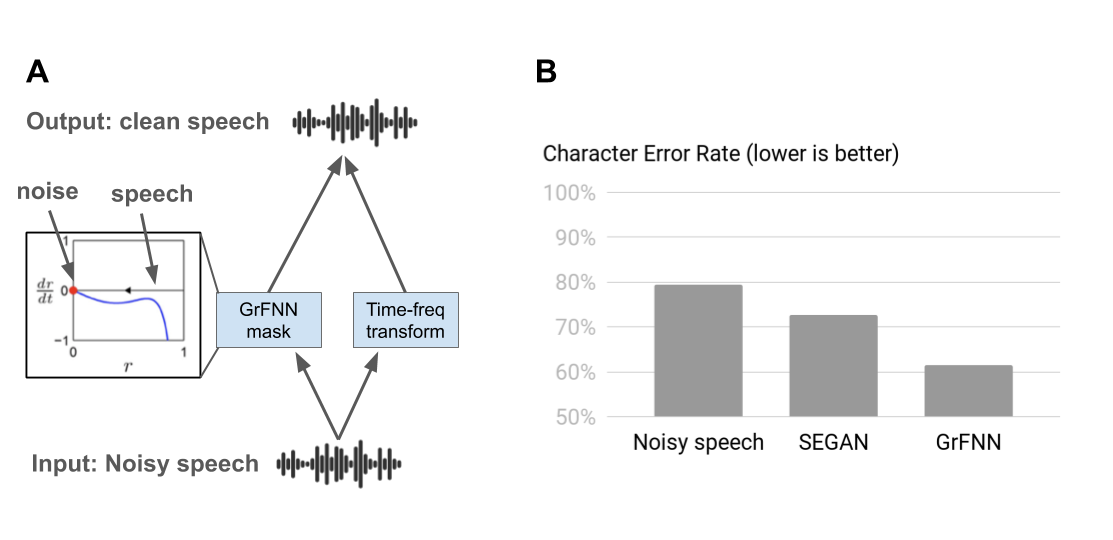
\includegraphics[width=1.0\textwidth]{figures/fig5_2.png}
    \caption[Speech enhancement with a GrFNN network optimized via gradient descent]{\textbf{Speech enhancement with a GrFNN network optimized via gradient descent.} (A) Model used for speech enhancement. The noisy speech signal is processed by a GrFNN network with double limit-cycle units that separate speech and noise to generate a time-frequency mask. In parallel, the time-frequency representation of the noisy signal is computed. Next, the GrFNN mask and the noisy time-frequency representation are combined to yield the enhanced speech. (B) CER performance of noisy speech, speech enhanced by SEGAN, and speech enhanced by our GrFNN model. The GrFNN outperforms SEGAN in the CER metric.}
    \label{f5_2}
\end{figure}

This second experiment shows that the parameters of different oscillators in a GrFNN network can be optimized simultaneously via gradient descent. In contrast with experiment 1 where no input signal was used and the steady state of the network was the training objective, in experiment 2 the GrFNN input was a dataset of speech utterances and the objective was the mean squared error between the enhanced speech and the ground-truth clean speech (see the methods section for more details that differentiated our two experiments). 

\section{Discussion}

\subsection{GrFNN parameters can be optimized with gradient descent}

Our new implementation of GrFNNs with tensorflow 2 allowed us to optimize GrFNN parameters with gradient descent and automatic differentiation in two very different experiments. These two experiments independently covered optimization of a single oscillator and a network of oscillators with and without stimulation, respectively. In the next sections we discuss the implications of these experiments.

\subsection{Experiment 1: Gradient descent optimization of a single GrFNN \\ oscillator to show limit-cycle activity} 


This simple experiment showed that the parameters of a single oscillator can be optimized with gradient descent to achieve a desired steady state behavior. Our results showed that the parameters required for a GrFNN to show unit magnitude limit-cycle behavior can be found through gradient descent if the objective function compares the amplitude of the oscillator with a desired limit-cycle amplitude. Results showed that $\alpha \approx 0.2$ and $\beta_1 \approx -0.2$ had similar values but with opposite signs, as expected \cite{kim2015signal}. What was not necessarily expected was the specific values to be around $0.2$. However, one can understand that this value is related to the time-constant with which the oscillator reaches the unit-magnitude amplitude from its initial conditions in Fig.{} \ref{f5_2} (see \cite{kim2015signal} for a description of the time constant dynamics in a GrFNN oscillator). Because the simulation lasted 10 seconds, the values of $\alpha$ needed to be around $0.2$ to ensure that the oscillator would reach the desired behavior by the end of the simulation. A simulation longer than 10 seconds would have resulted in a smaller magnitude of the $\alpha$ and $\beta_1$ parameters, while the opposite would have happened in a shorter stimulation. The other two parameters ($\beta_2$ and $\epsilon$) would have remained around zero because they are not relevant to the limit-cycle behavior.

Similar examples can be carried out to find parameters for all other possible behaviors that a GrFNN oscillator can show, including hopf bifurcation, limit-cycle, and double limit-cycles (see \cite{kim2015signal} for a complete description of possible states). Additionally, other parameters can be found through gradient descent. For example, if a stimulus exists, the stimulus amplitude to achieve a desired steady state could be found. Additionally, the frequency parameter of the oscillator could also be found in case the desired steady state activity has a specific frequency of activity. This first experiment demonstrates that gradient descent can optimally identify the parameters associated with steady states that are usually found by hand through stability analysis of a dynamical system. 

\subsection{Experiment 2: Gradient descent optimization of a GrFNN network \\ for speech enhancement.} 

In this experiment we used a network that did not have any intrinsic connections. Like in experiment 1, we optimized the individual oscillator parameters. Our results show that this is also possible at the network level. The objective function did not directly compare the GrFNN activity with a target, like in experiment 1. Instead, the GrFNN output was further processed to obtain an audio signal that was compared against another ground truth audio signal. Hence, this experiment shows that the activity of a GrFNN can be transformed by other computations in order to produce a higher order, more abstract output. In this experiment we also outperformed a particular deep learning method in a speech enhancement task (SEGAN \cite{pascual2017segan}). As a result, this second experiment also presents GrFNNs as a signal processing tool that can be optimized and combined with other operations. With this experiment we have showed that GrFNN parameters can be found using gradient descent with a data-driven and result-focused goal.

\subsection{General discussion}

We have presented a new toolbox to optimize GrFNNs with gradient descent in tensorflow 2. This new implementation opens the doors to expand the applications and topologies of GrFNNs. This was previously impractical due to the required steady state analysis to find parameters for all GrFNN oscillators in a complex model. Now gradient descent can do the parameter finding as long as we know which behavior we want to see from single oscillators or from a GrFNN network. We have shown how to build and optimize a single oscillator and a network of oscillators. Tensorflow also allows us to further process the GrFNN activity with mathematical functions and train GrFNNs parameters to generate abstract outputs typically used in machine learning, like classification categories or regression. A natural consequence of this toolbox is to use GrFNNs as time-frequency analyzers of signals in deep learning architectures. Because of their similarities to gammatone-filters and their tonotopy, GrFNNs could substitute time-frequency analysis methods like FFT, wavelet transforms, MFCCs, and mel filter-banks, all of which are usually the first step when processing raw audio in a deep learning architecture \cite{purwins2019deep}. 

This toolbox will also allow for the tensorflow implementation of networks of oscillatory models other than GrFNNs. Our runge-kutta integrator can integrate any ODE, and models relevant to neuroscience and biophysics are ODEs. We believe that our toolbox is the first step toward building a more robust and general tool for simulation of artificial biological systems. Additionally, other integrators (perhaps more appropriate for different types of models) could be written in addition to the fourth order runge kutta integrator that we implemented. The resulting simulations from our toolbox will have theoretical and practical applications in academic and industry settings. 

\section{Methods}

\subsection{Technical background}

Tensorflow was released in 2015 by Google as a free and open-source toolbox to build and train neural networks (and other kinds of machine learning models) \cite{abadi2016tensorflow}. Tensorflow allows for automatic differentiation of functions with respect to parameters, so that parameters can be updated and the function outputs match predetermined target values. To make this process as efficient as possible, tensorflow supports seamless GPU acceleration of these operations. Since its launch, communities of developers have contributed numerous features to tensorflow, primarily related to advances in deep learning research, allowing tensorflow to constantly be up to date with the most recent breakthroughs in artificial intelligence \cite{abadi2016tensorflow}. Tensorflow is currently in its second version (tensorflow 2.0, released in 2019), which provides multiple improvements over the previous version, including eager execution of code without needing a fixed graph and better GPU performance \cite{campesato2019tensorflow}.

While tensorflow was designed to optimize machine learning algorithms, one can compute any mathematical function using tensorflow. Considering this, Mohanta and Assisi \cite{mohanta2019parallel} proposed using tensorflow to streamline modeling of dynamical equations (usually ODEs or partial differential equations). Their idea is particularly motivated by the fact that in tensorflow one can define large networks of interacting units, or neurons, and such networks are automatically computed with GPU acceleration (assuming the right hardware and drivers are installed) without having to deal with any GPU code \cite{mohanta2019parallel}. They simulated a realistic model of an insect's olfactory system consisting of multiple types of neurons connected by different types of synapses \cite{mohanta2019parallel}. The results by Mohanta and Assisi \cite{mohanta2019parallel} demonstrate that one can use tensorflow as a scalable tool to compute a network consisting of thousands of coupled biological neurons (conductance-based models in their specific examples).

\subsection{Implementation}

Given that GrFNNs are ODEs and are originally derived from a model of neural oscillatory activity, we built upon Mohanta and Assisi's work \cite{mohanta2019parallel} to implement GrFNNs in tensorflow 2. We wrote a fourth order runge-kutta integrator that solves any arbitrary ODE by converting it into a tensorflow graph. All GrFNN parameters can be defined as tensorflow variables for every oscillator, and arbitrary parametric connections (static or ODE) can be specified between oscillators or even different GrFNN networks. The output activity of a GrFNN model can be further transformed by an objective function in order to compute an error term that can be used to optimize the values of GrFNN parameters. 

\subsection{Experiment 1: Gradient descent optimization of a single GrFNN \\ oscillator to show limit-cycle activity} 

\subsubsection{Task}

The goal of this experiment was to optimize the parameters of a single GrFNN oscillator to show unit magnitude limit-cycle activity at a frequency of 1Hz in a simulation that lasted 10 seconds. 

\subsubsection{Setup, procedure, and optimization}

We used our GrFNN implementation in tensorflow to define a single GrFNN oscillator like the one in Eq \eqref{eq:5.1}. The trainable parameters (or tensorflow variables) were $\alpha$, $\beta_1$, $\beta_2$, and $\epsilon$, all of which were initialized to be small random values close to zero. $\alpha$ and $\beta_1$ were drawn from a zero centered uniform distribution ranging from $-0.00001$ to $0.00001$. $\beta_2$ and $\epsilon$ are meant to be negative and positive, respectively \cite{kim2015signal}, so they were separately drawn from two uniform distributions, one ranging from $-0.00001$ to $0$ and the other one ranging from $0$ to $0.00001$. The frequency of the oscillator was fixed to be $f=1$, and the oscillator's initial conditions were a real and an imaginary number independently drawn from a gaussian distribution with mean of zero and variance of 1. In this simulation there was no stimulus (i.e., $x(t)=0$ in Eq \eqref{eq:5.1}). The resulting simulation was defined to last 10 seconds with a timestep of 0.05 seconds. To optimize the parameters, the oscillator was first integrated using the fourth order runge-kutta and the magnitude of the GrFNN oscillator during the last 6 timesteps was compared with an array of ones via mean squared error. Then, tensorflow automatically computed the gradients for the trainable parameters $\alpha$, $\beta_1$, $\beta_2$, and $\epsilon$, and updated its values using vanilla gradient descent. This procedure was repeated 100 times. 

\subsection{Experiment 2: Gradient descent optimization of a GrFNN network \\ for speech enhancement.} 

\subsubsection{Task}

In this experiment we optimized the parameters of a network of GrFNN oscillators to find the time-frequency mask that separated speech from pink noise.

\subsubsection{Setup, procedure, and optimization}

We defined a network of 78 GrFNN oscillators with frequencies logarithmically spaced from 64Hz to 8192Hz. The trainable parameters for each oscillator were $\alpha$, $\beta_1$, $\beta_2$, and $\epsilon$, which were initialized to be parameters associated with double limit-cycle dynamics (see \cite{kim2015signal}). The frequency of the oscillators was fixed, and all oscillators were initialized to be zero. The stimulus was a subset of 48 utterances from the TIMIT dataset \cite{garofolo1993timit} mixed with pink noise and a signal-to-noise ratio of 0dB. The resulting GrFNN simulations matched the length of the longest utterance in our dataset (all utterances were zero padded to match the longest utterance length) and had a sampling rate of 22050. All utterances were processed by the GrFNN, resulting in a time-frequency mask which then was multiplied element-wise with the time-frequency transformation of the corresponding noisy utterance. The resulting time-frequency map was converted back to the time domain, and the mean squared error between the GrFNN-processed utterance and the ground-truth clean version was computed. Tensorflow automatically found the gradient of all model parameters and used the gradient to optimize the parameter values. This process was repeated 200 epochs with an ADAM optimizer \cite{kingma2014adam} to find the best parameters. The 48 TIMIT utterances were run through the SEGAN model for speech enhancement to have a baseline comparison \cite{pascual2017segan}. Next, the noisy, the GrFNN enhanced, and the SEGAN enhanced versions of the TIMIT utterances were run through the DeepSpeech model \cite{hannun2014deep} to obtain character-based transcriptions. These transcriptions were compared against the DeepSpeech transcription of the clean version of the TIMIT utterances to assess the character error rate. 


\chapter{Conclusion}

\section{Summary of findings}
The three main studies presented in this dissertation were described in chapters 2, 3, and 5. The following subsections summarize the main findings of each of these chapters.

\subsection{Chapter 2}
This model showed that `strong anticipation' (the hypothesis explaining that anticipatory behavior is the result of coupling with delay \cite{stepp2010strong}) can capture human anticipatory tendencies when synchronizing movements with a metronome. Specifically, an oscillatory model with delayed feedback resulted in anticipatory behavior when synchronizing with a periodic stimulus. Moreover, two different amplitudes for the delayed feedback term allowed us to simulate the different anticipatory tendencies observed in musicians and non-musicians. The smaller delayed feedback amplitude simulated the musician anticipation and a larger delayed feedback amplitude simulated the non-musician anticipation. 
    
The same model and the same parameters were used to simulate different musical behaviors in solo and group settings. One of the behaviors involved transmission delays, which cancel out the anticipatory tendency due to the extra time it takes for two synchronizing parties to hear each other's actions. The model could also make predictions about human behavioral data not yet collected, specifically for tasks where musician data exists, but non-musician data is still missing. Thus, our model predictions can be validated in the future by collecting this missing data.

\subsection{Chapter 3}
This model demonstrated how the spontaneous motor tempo (SMT) systematically affects the tempo of musicians performing simple melodies. Our oscillatory model simulated the SMT with the oscillator natural tempo (ONT). We used Hebbian learning to adaptively adjust the model tempo and match the stimulus tempo. Additionally, the model also had an elastic force constantly pulling the model tempo to its ONT. This resulted in our model anticipating stimuli slower than the ONT, and lagging stimuli faster than the ONT. Additionally, in the absence of a stimulus, the model had a tendency to return to its ONT. Finally, when two of these models synchronized with each other, the difference between the two models' ONTs was proportional to the absolute asynchrony observed between the models.

We used the same model and the same set of parameters to simulate human tasks previously described in the literature. All our simulations and observations made with our model were consistent with the existing human data. Additionally, we also used our model to make predictions about human data that has not yet been collected, and these predictions can be tested in the future by collecting the missing human data.
    
\subsection{Chapter 5}
We implemented the first tensorflow library of neural oscillators, allowing for optimization of oscillatory networks parameters via automatic differentiation and gradient descent. We observed that using gradient descent optimization one can identify model parameters for well-known oscillatory dynamics like limit-cycles. Additionally, one can use gradient descent to find parameters for oscillatory networks using an objective function and a data-driven approach.

\section{Contributions}
This dissertation ultimately has a set of contributions to the fields of dynamical systems modeling of human behavior and signal processing. 

\subsection{Strong anticipation in human behavior}
We have demonstrated that one can use a dynamical system with delayed feedback to simulate human anticipation during perception-action coordination. We only needed to add delayed feedback to an oscillator in order to capture human anticipation. A more complex mechanism of anticipation, like statistical inference, was not necessary. Knowing that delayed feedback causes anticipation tendencies in humans means that we can hypothetically measure axonal delays and make predictions about anticipatory behavior. Conversely, we can also hypothetically measure anticipation tendencies and predict a person's axonal delays. 

Using the same model we simulated human anticipation in solo and interpersonal perception action coordination tasks. We captured three very different experiments using the same set of parameters. Our model is simple and parsimonious because it uses an oscillator that has previously been studied in the literature, and we only added a delay to this oscillator in order to observe anticipacion. 

\subsection{Elastic Hebbian tempo learning}
We have identified the mechanisms that relate the spontaneous motor tempo (SMT) to actions requiring musicians to maintain a musical tempo. The mechanisms are adaptive tempo learning and an elastic force constantly pulling to an individual's SMT. Similar to the strong anticipation model, this model also accounts for a variety of synchronizing behaviors observed in real human data in solo and interpersonal settings.

\subsection{Gradient descent optimization of oscillator networks}
Our implementation will allow for data-driven and large-scale optimization of oscillatory networks as well as other dynamical system models. This new implementation will also allow for the integration of oscillatory networks in deep learning and machine learning algorithms. In the specific case of gradient frequency neural networks (GrFNNs), their dynamics could lead to major advancements in the spectral processing of signals in the feature extraction layers of common deep learning algorithms for speech and music applications


\appendix
\chapter{Supplementary figures}
\begin{figure}
    \centering
    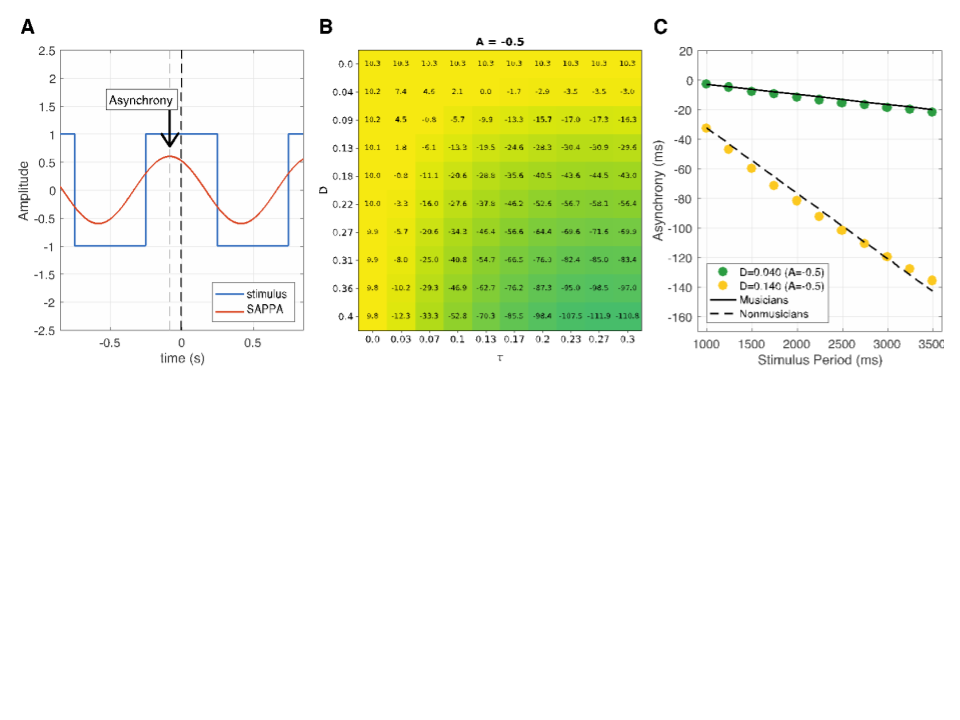
\includegraphics[width=1.0\textwidth]{figures/figS_1.png}
    \caption[The SAPPA model's behavior when the external periodic input is a square wave instead of a sinusoid]{\textbf{The SAPPA model's behavior when the external periodic input is a square wave instead of a sinusoid.} (A) Illustration of what the asynchrony between the SAPPA model and the external square wave stimulus looks like, and how it's measured. (B) Analysis of the asynchrony (in ms) as a function of $D$ and $\tau$ in Eq \eqref{eq:2.5} when $A = -0.5$ and $f = 1$. (C) The anticipation observed when the musician (green dots) and non-musician (yellow dots) SAPPA models were stimulated by the external square wave while also receiving their own non-delayed activity as input ($A = -0.5$). In all simulations $\tau = 0.222$ seconds. The $D$ parameter differentiates the musician and non-musician models. The regression lines for the behavioral data originally shown in Fig.{} \ref{f2_1}A are shown for comparison purposes in (C).}
    \label{fS_1}
\end{figure}

\begin{figure}
    \centering
    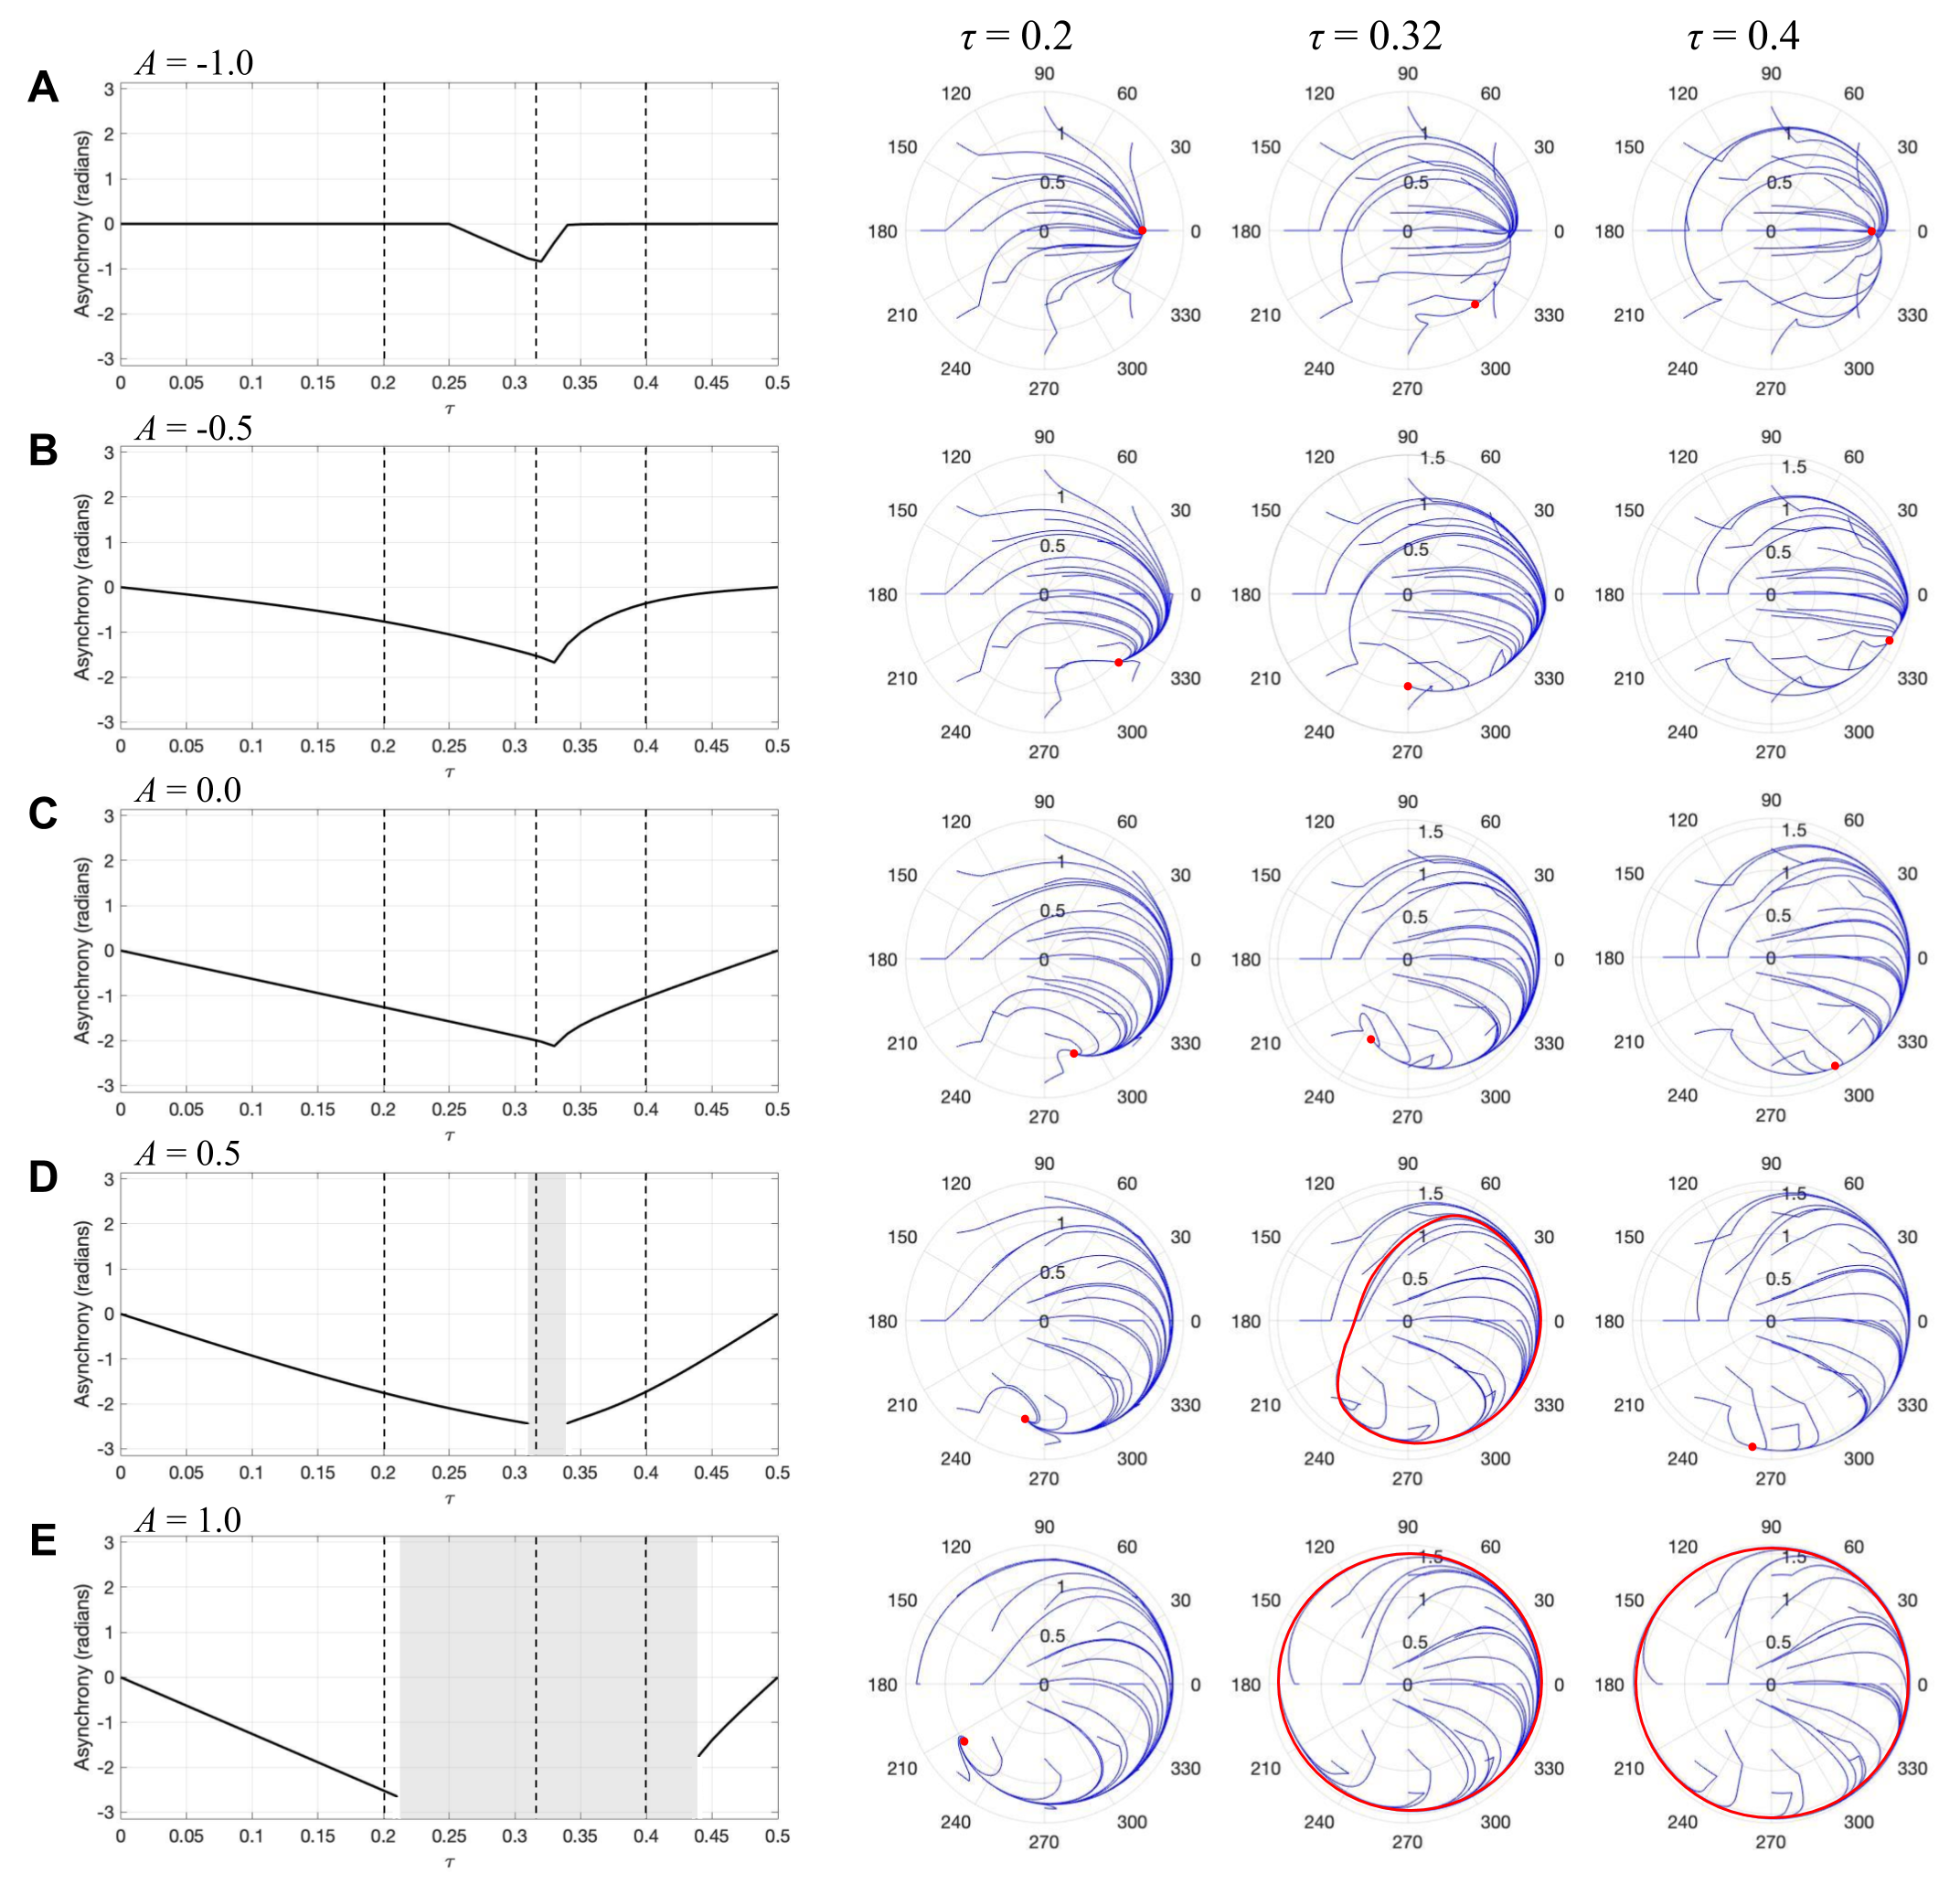
\includegraphics[width=1.0\textwidth]{figures/figS_2.png}
    \caption[Analysis of the asynchrony between the SAPPA model and the stimulus as a function of the recurrent delay $\tau$]{\textbf{Analysis of the asynchrony between the SAPPA model and the stimulus as a function of the recurrent delay $\tau$.} Rectangular plots (left panels) show the asynchrony as a function of $\tau$ (in units of seconds) for different values of $A$ while $D$ stays constant ($D = 1.0$; $f = 1.0$). Circular plots (right panels) show the angle of the asynchrony and the magnitude of the SAPPA model. In the rectangular plots, asynchrony is shown in units of radians, and not in seconds, in order to match the cyclic dynamic range of the circular plots. In the rectangular plots, gray-shaded areas indicate regions where the SAPPA model did not synchronize with the stimulus, and instead mode-locking was observed. Vertical dotted lines indicate values of $\tau$ for which circular plots were calculated. In the circular plots, individual blue lines start from different initial conditions, all of which arrive to either a red dot (a fixed point) or a red ring (a limit cycle). (A) $A = -1.0$ (B) $A = -0.5$ (C) $A = 0.0$ (D) $A = 0.5$ (E) $A = 1.0$. The limit cycle behavior is observed when the SAPPA model does not synchronize with the stimulus, and instead the SAPPA model mode-locks with the stimulus. Note: the circular plots are known as polar plots.}
    \label{fS_2}
\end{figure}

\bibliographystyle{unsrt}
\bibliography{mybib}
\end{document}
